\input{/Users/daniel/github/config/preamble.sty}%This is available at github.com/danimalabares/config
\input{/Users/daniel/github/config/thms-eng.sty}%This is available at github.com/danimalabares/config

\begin{document}

\begin{minipage}{\textwidth}
	\begin{minipage}{1\textwidth}
		 \hfill 		
		{\small\hfill\href{https://github.com/danimalabares/seminars}{github.com/danimalabares/seminars}}

		
		%{\small\hfill\href{https://github.com/Friday-seminar/}{github.com/Friday-seminar}}
	\end{minipage}
\end{minipage}\vspace{.2cm}\hrule

{\Huge Notes on seminars}

{\large (and what-not)}
\phantomsection
\tableofcontents

\clearpage\phantomsection\stepcounter{section}\addcontentsline{toc}{section}{\thesection\quad Classification of log Calabi-Yau pairs}\addtocontents{toc}{\hspace{1em}\textit{Eduardo Alvez da Silva, \hspace{.2 em}Institut de Mathématiques d'Orsay,\hspace{.5em}September 6, 2024, Friday Seminar}\par}
{\Huge Classification of log Calabi-Yau pairs}

\hfill{\Large Eduardo Alvez da Silva}

{\Large \hfill Institut de Mathématiques d'Orsay}

\hfill{\large September 6, 2024

\hfill \textit{Friday Seminar}}

\subsection{Introduction}


\begin{defn}
	A \textit{\textbf{log Calabi-Yau}} pair is a lc pair  $(X,D)$ consisting of a normal projective variety $X$ and a reduced Weil divisor $D$ such that $K_X+D\sim_{\mathbb{Z}}0$.
\end{defn}

\begin{remark}
	Let $n=\dim X$. $(X,D)$ CY pair $\implies $ $\exists \omega:=\omega_{X,D}\in\Omega^n_x$, unique up to nonzero scaling such that $\operatorname{div}(\omega)+D=0$. We call $\omega$ the \textit{\textbf{volume form}}.
\end{remark}

\[\begin{tikzcd}
	(X,D)\text{minimal model}& \arrow[l,"\text{log MMP}" ](X,D)\text{ CY pair} \arrow[r,"\substack{\text{Classical}\\\text{MMP/X}}"  ]&\text{Mori fibered space} 
\end{tikzcd}\]

\begin{itemize}
	\item $(X,D)$ CY pair,
\begin{align*}
	K_{X}+D\sim 0 &\implies -K_X=D\geq 0\\
	&\implies K_X\text{ is not pseudo effective}\\
	&\overset{*}{\implies } X \text{is uniruled}\\
	&\implies K(X)=-\infty\\
	&\implies \text{The output of the  MMP over $X$ is Mori fibered space} 
\end{align*}
where $*$ means BDPP theorem.

	\item $(X,D)$ is a minimal model for the log MMP since $K_X+D$ is nef.
\end{itemize}

\begin{example}
	[content…]
\end{example}

\begin{defn}
	Let $f:(X,D_X)\overset{\operatorname{bir}}{\longrightarrow}(Y,D_Y)$ be a birational map of CY pairs. $f$ is \textit{\textbf{volume preserving}} if $f^* \omega_{Y,D_Y}$, for some $\lambda\in\mathbb{C}^*$.
\end{defn}

\begin{remark}
	$\operatorname{Bir}^{\operatorname{up}}(X,D_X) \subset \operatorname{Bir}(X)=$group of all volume-preserving maps.
\end{remark}

\begin{defn}[Other equivalent definitions]\leavevmode 
	\begin{enumerate}[label=(\roman*)]
		\item $f$ \textit{\textbf{preserves discrepancies}}, i.e. for a divisor  $E$ over $X$ and $Y$ we have $a(E,X,D_X)=a(E,Y,D_Y)$.

		\item $f$ admits a log resolution
			\[\begin{tikzcd}
				& (Z,D_Z)\arrow[dr,"vq"]\arrow[dl,"up"]\\
				(X,D_X)\arrow[rr,dashed]&&(Y,D_Y)
			\end{tikzcd}\]
			\[up^*(K_X+D_X)=q^*(K_Y+D_Y)\]

			\paragraph{Warning} $D_Z$ does not need to be effective. Ex. look at my PhD thesis in section 5.4.

			\paragraph{Notation.} Volume preserving equivalence, or crepant birrational,
			\[(X,D_X)\cong_{\operatorname{vp}}(Y,D_Y)\]
			\[(X,D_X)\cong_{\operatorname{cbir}}(Y,D_Y)\]
			Because volume-preserving maps are also called crepant maps.

	\end{enumerate}
\end{defn}

\paragraph{Problem} (Very hard!) Classification of log CY pairs up to volume-preserving equivalence.

The most important invariant to attack this problem is the following:

\begin{defn}
	The \textit{\textbf{corregularity}} of a log CY pair $(X,D_X)$, $\operatorname{coreg}(X,D_X)$, is defined to be the dimension of a minimal lc center in a dlt modification
	\[f:(X^{\operatorname{dlt}},D_{X^{\operatorname{dlt}}})\to (X,D_X)\]
\end{defn}

\begin{remark}
	$c:=\operatorname{coreg}(X,D_X)$, $0\leq c\leq \dim X$, $c=\dim X\iff X$ is CY and $D_X=0$.
\end{remark}

\subsection{Classification of log CY pairs in dimension 2}

After a minimal resolution of singularities, it follows that a surface log CY pair $(X,D_X)$ is agiven by one of the following:

\begin{itemize}
	\item $c=2$: X is an abelian surface or a K3 surface, and $D_X=0$.

	\item $c=1$:
		 \begin{enumerate}[label=(\roman*)]
			\item $X$ is rational and $D_X\in |-K_X|$ is a nonsingular elliptic curve.
			\item $\pi:X\to E$ (not necessarily minimal) ruled surface over a nonsingular elliptic curve $E$, and $D_X=D_1+D_\alpha\in |-K_{X}|$ is the sum of two disjoint sections of $ \pi$.
		\end{enumerate}
	
	\item $c=0$:  $X$ is rational and $D_X$ is a (possible reducible) nodal curve of arithmetic genus 1.
\end{itemize}

\begin{example}
	$X=\mathbb{P}^2$. Three lines, conic + line, nodal cubic, nonsingular cubic. Their corregularities are zero except for the last one, which is 1.
\end{example}

\begin{defn}
A log CY pair $(X,D_X)$ has a \textit{\textbf{toric model}} if $(X,D_X)\cong_{\operatorname{vp}}(T,D_T)$ (where $D_T$ is the reduced sum of all torus invariant divisors).
\end{defn}

\begin{thm}[Gross-Hacking-Keel]\leavevmode
	Every surface log CY pair $(X,D_X)$ of log coregularity 0 has a toric model.
\end{thm}

\begin{remark}
	Its false in dimension $\geq 3$.
\end{remark}

\subsection{(Partial) Classification in dimension 3}

\begin{thm}[Ducat, 2023]\leavevmode
	Let $(\mathbb{P}^3,D)$ be a log CY pair with corregularity $c\leq 1$. Then there exists a volume-preserving map
	\[\varphi:(\mathbb{P}^3,D)\overset{bir}{\longrightarrow}(\mathbb{P}^1\times \mathbb{P}^1,D') \]
	where
	\[D'=(\{0\} \times \mathbb{P}^1)+(\mathbb{P}^1+E)+(\{\infty\} \times \mathbb{P}^2)\in |-K_{\mathbb{P}^4\times \mathbb{P}^2}|\]
	for a plane cubic $E\subset \mathbb{P}^2_{(x:y:z)}$ such that
	\begin{enumerate}
		\item  $c=1\iff$ $E$ is non singular.

		\item If $c=0$, then $E=\{xyz=0\}$. In particular $D'$ is the toric boundary of $(\mathbb{P}^1\times \mathbb{P}^2$ and thus $(\mathbb{P}^3,D)$ has a toric model.

		\item $c=2$ (The missing case) Fact:  $c=2\iff D$ is an irreducible normal quantic surface having canonical singularities, i.e., $D$ is either nonsingular or has ADE singularities $ \iff$ the pair is canonical
	\end{enumerate}
\end{thm}

\begin{example}[Oguiso's example]
	He constructed two nonsingular isomorphic quartic surfaces $D,D'\subset \mathbb{P}^3$ (as abstract varieties) such that there exists $\varphi \in\operatorname{Bir}(\mathbb{P}^3)$ mapping $D$ birrationally onto $D'$ $\implies $ $(\mathbb{P}^3,D)\not\cong_{\operatorname{vp}} (\mathbb{P}^3,D')$.
\end{example}

	Thinking in terms of coarse moduli spaces, we have a natural map
	\begin{align*}
		\mathcal{M}_{(\mathbb{P}^3,D)}^{c=2}  &\longrightarrow  \mathcal{M}_{K3}^{\operatorname{can}}\\
		[(\mathbb{P}^3,D)] &\longmapsto [D]
	\end{align*}
	and Oguiso's example implies that this is not injective.

\begin{conjecture}[Trichotomy]
\leavevmode 

\begin{table}[H]
	\centering
	\begin{tabular}{c|ccc}
		$\operatorname{coreg}(\mathbb{P}^3,D)$&0&0&?\\
		$\dim \mathcal{M}_{(\mathbb{P}^3,D)}^c$ &0&1&?\\
		$\operatorname{Bir}^{\operatorname{vp}}$ &monstruous&?&$\operatorname{Dec}(D)$ \\
		\hline
		$g$&0&1&$\geq 2$\\
		$\dim \mathcal{M}_{g}$ &0&1&$3g-3$\\
	$\operatorname{Bir}=\operatorname{Aut}$ &$\operatorname{PGL}(2,\mathbb{C})$ infinite&$C\rtimes\mathbb{Z}_d$&\#$\operatorname{Aut}(C)\leq 84(g-1)$ finite
	\end{tabular}
\end{table}
\end{conjecture}

$D$ very gen. $D$ is nonsingular,
\[\varphi:(\mathbb{P}^3,D)\overset{\operatorname{v.p}, \operatorname{bir}}{\longrightarrow}(\mathbb{P}^3,D)\] 
\[\implies \varphi |_D D\overset{\cong }{\longrightarrow}D\]
$X$ projective variety, $Y\subset X$ irreducible subvarieties,
\[\operatorname{Bir}(Y,X)=\{f\in\operatorname{Bir}(X)|f|_Y:Y\overset{\operatorname{bir}}{\longrightarrow}Y\}\]

\begin{conjecture}[Shokuroo]
	Every 3-fold rational log CY pair $(X,D_X)$ of coregularity 0 has a toric model.
\end{conjecture}

Ducat's Theorem implies it is tru for $X=\mathbb{P}^3$.

\begin{defn}
	$(X,D_X)$ CY pair, $D_X=D_1+\ldots+D_r$. The \textit{\textbf{complexity}} of this CY pair is the non-negative number
	\[c(X,D_X):=\dim X+\operatorname{rk}(\operatorname{Cl}(X)_{\mathbb{Q}})-r\]
\end{defn}

\paragraph{Fact} $c(X,D_X)=0\implies (X,D _X)$ has a toric model (Brown, Mckenan, Lvald, Long, 2018).

\begin{defn}
	$(X,D_X)$ CY pair. The \textit{\textbf{birrational complexity}} is 
	\[c_{\operatorname{bir}}(X,D_X):=\min\{c(Y,D_Y)|(Y,D_Y)\cong_{\operatorname{vp}}(X,D_X)\}\]
\end{defn}

\begin{thm}[Mauri, Moraga, 2023]\leavevmode
	$c_{\operatorname{bir}}(X,D_X)=0\iff(X,D_X)$ has a toric model.
\end{thm}

\begin{defn}
	A log CY pair $(X,D_X)$ is \textit{\textbf{cluster type}} if there exists a volume-preserving map
	\begin{align*}
		\varphi: (\mathbb{P}^n,H_0+\ldots+H_{n+1} &\overset{\operatorname{bir}}{\longrightarrow}(X,D_X) 
	\end{align*}
such that $\operatorname{codim}_{\mathbb{C}^n_M}(\operatorname{Ex}(\varphi )\cap \mathbb{C}^n_m)\geq 2\iff \mathbb{C}^n_m\hookrightarrow X\setminus D_X$.
	
\end{defn}

\begin{thm}[---,Figueroa, Moraga, 2024]\leavevmode
	$(\mathbb{P}^3,D)$ log CY pair of coregularity 0.  Assume $D$ general in its deformation class. Then $(\mathbb{P}^3,D)$ is cluster type unless one of the following happens:
	\begin{enumerate}[label=(\roman*)]
		\item $D$ reducible, $D=H+C$ (plane cubic, resp.) such that $H\cap C$ is a nodal plane cubic.

		\item $D$ irreducible and has double points along a line.
	\end{enumerate}
\end{thm}

\subsection{Sketch}

\begin{align*}
	(\mathbb{P}^3,D)\text{is cluster type}  &\iff(\mathbb{P}^3,D) \text{ is cluster type over}\mathbb{P}^1\\
	&\iff\exists \text{ some dlt modification } (X,D_X)\\
	&\text{of $\mathbb{P}^3$ such that $\exists $ a crepant contraction}\\
	&\text{onto $(\mathbb{P}^4,\{C\} +\{\infty\} )$} .
\end{align*}

\clearpage\phantomsection\stepcounter{section}\addcontentsline{toc}{section}{\thesection\quad Jacobian elliptic fibrations on K3s with a non-symplectic automorphism of primer order}\addtocontents{toc}{\hspace{1em}\textit{Felipe Zingali Meira, \hspace{.2 em}UFRJ,\hspace{.5em}September 20, 2024, Seminário das Sextas}\par}
{\Huge Jacobian elliptic fibrations on K3s with a non-symplectic automorphism of primer order}

\hfill{\Large Felipe Zingali Meira}

{\Large \hfill UFRJ}

\hfill{\large September 20, 2024

\hfill \textit{Seminário das Sextas}}

\vspace{2em}

\begin{thing4}{Abstract}
K3 surfaces are one of the few classes of algebraic surfaces which allow more than one distinct relatively minimal elliptic fibration. There are distinct ways of classifying such fibrations. In this talk, we will describe how to classify these fibrations with relation to the action of a non-symplectic automorphism $\sigma$ of prime order on a K3 surface $X$, and how each type of fibration relates to a linear system in the quotient surface $X/\sigma$.
\end{thing4}
\vspace{2em}

\begin{figure}[H]
	\centering
	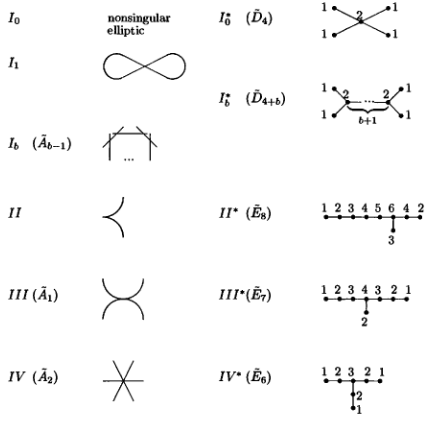
\includegraphics[width=0.6\textwidth]{elliptic.png}
	\caption*{\href{https://www.math.columbia.edu/~chaoli/docs/EllipticSurfaces.html}{Kodaira classification of fibers}}
\end{figure}

\subsection{Definitions}

\begin{defn}
	Let $S$ be a projective smooth surface and $C$ a projective smooth curve. An \textit{\textbf{ elliptic fibration}} is a surfective map $\mathcal{E}:S\to C$ such that
	\begin{enumerate}[label=(\roman*)]
		\item All but finitely many fibres $F_{v}=\mathcal{E}^{-1}$ are irreducible genus 1 curves.
		\item $\mathcal{E}$ is \textit{\textbf{Jacobian}} if there is a section $s_0:C\to  S$.
		\item $\mathcal{E}$ is \textit{\textbf{relatively minimal}} if no fibre contains a $(-1)$-curve.
	\end{enumerate}
\end{defn}

The generic fiber of such a fibration is a genus 1 curve over the function field of the curve $E/K(C)$. Then there is a one-to-one correspondence
\[\{\text{pts in $E(K(x))$}\overset{\text{1-1} }{\longleftrightarrow }\} \{\text{sections $s:C\to S$} \}\]

Drawing of this fibration: base space is a curve, total space is a family of elliptic curves. Section is a curve that takes one point from every elliptic curve in total space.

\begin{enumerate}
	\item $K_S=(\chi(s)-2)F$,  $F$ is the fiber class in $\operatorname{NS}(S)$. Recall that Neron-Severi group is divisors quotient linear equivalence, but in this case perhaps we can just take it to be Picard group.
\item $\operatorname{NS}(S)$ is a lattice with the intersection pairing.
	\item $\operatorname{Triv}(S)=\left<\Sigma_0,F\right> \oplus \left<\text{components of reducible fibers} \right> $.
		\[\dfrac{\operatorname{NS}(S)}{\operatorname{Triv}(S)}\cong E(K(C))\]
		and also we have the formula
		\[\rho(S)=2+r+\sum m_v-1\]
	\item $e(S)=\chi_{\text{tod} }(S)=\sum_{v\in C}e^{F_v}$ where $\chi(S)=\frac{e(S)}{12}+k^2_S$
	\item 
\end{enumerate}

\subsection{Rational elliptic surfaces}

\begin{defn}
	Let $R$ be a rational surface (nonsingular projective) with an elliptic fibration $\mathcal{E}:R\to \mathbb{P}^1$.
\end{defn}

\begin{example}
	Let $f,g$ be cubics in  $\mathbb{P}^2$ and take the rational map
	\begin{align*}
		\varphi: \mathbb{P}^2 &\overset{\operatorname{rat}}{\longrightarrow} \mathbb{P}^1 \\
		p &\longmapsto [f(p):g(p)]
	\end{align*}
	\[\begin{tikzcd}
	&R\arrow[dl,"\eta",swap]\arrow[dr,"\mathcal{E}"]\\
	\mathbb{P}^2\arrow[rr,"\varphi"]&&\mathbb{P}^1
	\end{tikzcd}\]
\end{example}

\paragraph{Over $k=\bar{k}$} Every RES which is rel. min. + Jacobian is constructed by blowing up the base points of a cubir pencil. $\rho(R)=10$.

\subsection{K3 surfaces}

\begin{quotation}
	An important subclass of K3 surfaces, easier to analyze than the general case, consists of the K3 surfaces with an elliptic fibration $X\to \mathbb{P}^1$. "Elliptic" means that all but finitely many fibers of this morphism are smooth curves of genus 1. The singular fibers are unions of rational curves, with the possible types of singular fibers classified by Kodaira.
	
	\hfill \href{https://en.wikipedia.org/wiki/K3_surface#Elliptic_K3_surfaces}{wiki}
\end{quotation}


\begin{defn}
	A \textit{\textbf{K3 surface}} is a smooth projective surface such that
	\begin{itemize}
	\item $q(X):=h^1(X,\mathcal{O}_X)=0$.

	\item $K_X=0$, ie. there exists  $\omega_X\in H^{0}(X,\Omega^2_X)$ non-vanishing.
	\end{itemize}
\end{defn}

\begin{prop}
	$\mathcal{E}:X\to \mathbb{P}^1$ Jacobin, rel. min. Then
	\[X \text{ is a K3}\iff e(X)=24 \]
	\[q(X)= h^{1}(X,\mathcal{O}_X)=h^{2}(X,\mathcal{O}_X)+h^{0}(X,\mathcal{O}_X)-\chi(X)=1+1-2=0\]
\end{prop}

\begin{defn}
Let $X$ be a K3 surface and $\sigma\in\operatorname{Aut}(X)$ such that
\[\sigma ^*(\omega_X)=\xi \omega_X,\qquad \xi \text{ root of unity,} \]
We say 
\begin{itemize}
\item $\sigma$ is \textit{\textbf{symplectic}} if $\xi =1$.
\item $\sigma$ is \textit{\textbf{non-symplectic}} otherwise.
\end{itemize}

Suppose $\sigma\in\operatorname{Aut}(X)$ with finite order $\operatorname{ord}\sigma=n$.
\[X/\sigma=\begin{cases}
	\text{K3 if $\sigma$ is symplectic}\\
	\text{Rational if $n\geq 3$ or $n=2$ and $\operatorname{Fix}(\sigma)\neq \varnothing $}\\
	\text{Enrigues if $n=2$ and $\operatorname{Fix}(\sigma)=\varnothing $} 
	\qquad &
\end{cases}\]
\end{defn}

\subsection{Base change}

How to build K3 surfaces out of…

\[\mathcal{E}:R\to \mathbb{P}^1,\qquad \qquad \tau :\mathbb{P}^1\to \mathbb{P}^1 \text{ $n-1$ cover} \]
\[\begin{tikzcd}
	R\arrow[d,"\mathcal{E}",swap]& R\times_{\mathbb{P}^1}\mathbb{P}^1\arrow[l]\arrow[d]& Y\arrow[d]\\
	\mathbb{P}^1&\mathbb{P}^1\arrow[l,"\tau ",swap]& X\arrow[l,swap,"\mathcal{E}_X"]
\end{tikzcd}\]

\begin{remark}[Sergey]\leavevmode
	That fibered product may have singularities at the critical points of $\mathcal{E}$ and $\tau$, ie. any point that is collapsed in the quotient (definition of fibered product).
\end{remark}

	We can tell the Kodaira type of a fiber $\mathcal{E}^{-1}_X(v)=F^X_v$ by knowing
	\begin{itemize}
	\item the kodaira type of $\mathcal{E}^{-1}(u):=F_u$, $u=\tau(v)$.
	\item The ramification index $r(v|u)$
	\end{itemize}

	There are tables on how to determine the Kodaira types from that.

*Several drawings*

\paragraph{$n=3$} $\mathcal{E}_{x}:X\to \mathbb{P}^1$ is a K3 if
\begin{itemize}
\item $F_a^x$ is of type IV or $I^*_n$ and $F^x_b$ is at type $I_n, \operatorname{I I},\operatorname{I I I }$.
\end{itemize}

\subsection{Towards the classification}

\begin{defn}
$(X,\sigma)$, $X$ a K3 surface, $\sigma\in\operatorname{Aut}(X)$, $\operatorname{ord}(\sigma)=p$ prime, $\sigma$ non-symplectic. $\mathcal{E}:X\to \mathbb{P}^1$ a Jacobian ell. fib. (by K3 surface condition it is relatively minimal via adjunction formula). Then

\begin{itemize}
\item $\mathcal{E}$ is of \textit{\textbf{type 1}} if $\sigma^*(F)=F$ and $\sigma$ acts trivially on $\mathbb{P}^1$.
\item $\mathcal{E}$ of \textit{\textbf{type 2}} if  $\sigma^*(F)=F$ and $\sigma$ acts on $\mathbb{P}^1$ with order $p$.
\item $\mathcal{E}$ is of \textit{\textbf{type 3}} if $\sigma^*(F)\neq F$.
\end{itemize}
\end{defn}

Three drawings to show the types. Type one moves a point in a fiber to a another point the fiber, while fixing the base point of the fiber. Type 2 moves points from one fiber to another, and also maps the base points one to another. Type 3 is more messy, moves points from a fiber to the horizontal curves (sections)

\paragraph{Assumption:} acts trivially on $\operatorname{NS}(X)$ (Sarti, Arteloni, Taki).

\subsection{Type 1}
$F_v$ nonsingular, $\sigma$ acts on $F_v$ the order of an automorphism of an elliptic curve is 2,3,4,6 the order of an automorphism of an elliptic curve is 2,3,4,6.

When $p=2$, Garbognati, Salgado 17, Fibre types of  $F_v$ are $\operatorname{I}n,\operatorname{I}n^* ,\operatorname{I I I}$.

When $p=3$, 24, and types $\operatorname{I},\operatorname{I I}^* ,\operatorname{IV},\operatorname{IV}^* ,\operatorname{I}_{0},\operatorname{I}_{0}^*$.

$X/\sigma$, $\operatorname{ord}(\sigma)\geq 3$. Then $\operatorname{Fix}(\sigma)$ allows isolated fixed points
\[\operatorname{Fix}(\sigma)=C^1_g \cup c_1\cup \ldots \cup c_n\cup \{p_1,\ldots,p_k\}\]
where $C^1_g$ is a curve of genus $g$ and $C_1,\ldots,C_k$ are rational curves.

When $p=2$, $\operatorname{Fix}(\sigma)\neq \varnothing$.

$X/\sigma=\tilde{R}$ is rational and smooth.
\[\begin{tikzcd}
	\tilde{R}\arrow[d]&\tilde{X}\arrow[l,"\hat{\pi}"]\arrow[d]\\
	X/\sigma & X\arrow[l,"\pi"]
\end{tikzcd}\]

$ \mathcal{E}:X\to \mathbb{P}^1$ induces a linear system of curves $\Lambda$ in $\tilde{R}$.

\begin{enumerate}
	\item  $\mathcal{E}$ of type 1 $\implies \Lambda$ pencil of conics.
	\item $\mathcal{E}$ of type 2 $\implies \Lambda$ pencil of genus 1 curves.
	\item $\mathcal{E}$ of type 3 $\implies \Lambda$ is a non-complete linear system.

	\item 
\end{enumerate}

\subsection{Type II}

*Computations and discussion*

$\mathcal{E}:X\to \mathbb{P}^1$ of type  II induces a Jacobian elliptic fibration. $\mathcal{E}_{\tilde{R}}:\tilde{R}\to \mathbb{P}^1$ blow down to a rel. minimal $\mathcal{E}_R:R\to \mathbb{P}^1$.

Let $\tau :\mathbb{P}^1\to \mathbb{P}^1$ be the quotient by the action of $\sigma$ in $\mathbb{P}^1$.
\[\begin{tikzcd}
	R\arrow[d,swap,"\mathcal{E}_R"]& R\times_{\mathbb{P}^1}\mathbb{P}^1\arrow[l]\arrow[d]\\
	\mathbb{P}^1&\mathbb{P}^1\arrow[l,"\tau "]
\end{tikzcd}\]
I obtain $\mathcal{E}:X\to \mathbb{P}^1$ back.

Let $F_a^X,F_b^X$ be the ramified fibers of $\mathcal{E}:X\to \mathbb{P}^1$ of type 2. $\operatorname{ord}(\sigma)=3$.
\begin{itemize}
\item $F^X_a$ is of type $\operatorname{I}^*_{3n}$ or $\operatorname{I}_{0}$.
\item $F^X_b$ is of type $\operatorname{I}_{3n},\operatorname{I}^*_{0}$ or $\operatorname{I I I}$.
\item Every other fibre is irreducible.

	*Drawing using a base change*
\end{itemize}

\subsection{A concrete example of everything happening}

Start by building a rational elliptic surface, base change it, look at the K3 surface that's going to appear, and this K3 look at different elliptic fibrations and see what types they will have.

Start with $\mathbb{P}^2$ and
\begin{align*}
	f:xyz&=0\\
	g:(x-y)(y-z)(z-x)&=0
\end{align*}

Drawings of these curves and then of the K3 surface obtained after base change. The reasons why the intersections are as drawn is more involved.

$\Gamma$ pencil of curves in $\mathbb{P}^2$ induced by $\mathcal{C}_{|M'|}:X\to \mathbb{P}^1$ 
\begin{itemize}
\item $\mathcal{C}_{a}$ image of $\mathcal{G}_{a}$.

\item $\mathcal{C}_{0}$ image of $\mathcal{G}_{a}$ 

	These two imply $\Gamma:s\mathcal{C}_{a}+t\mathcal{C}_{b}$ 

\item The generic fibre of $\mathcal{C}_{|M'|}$ is given by
	\[s^3\mathcal{C}_a+t^3\mathcal{C}_b\]
	\[y^2=x^3+A(t^3)x+B(t^3)\]
	\[(x,y,t)\mapsto (x,y,\xi_3t\]
\end{itemize}

*I had to leave the talk*



\clearpage\phantomsection\stepcounter{section}\addcontentsline{toc}{section}{\thesection\quad Degenerations of the canonical series for curves (Part 1/2)}\addtocontents{toc}{\hspace{1em}\textit{Eduardo Esteves, \hspace{.2 em}IMPA,\hspace{.5em}September 20, 2024, Seminário das Sextas}\par}
{\Huge Degenerations of the canonical series for curves (Part 1/2)}

\hfill{\Large Eduardo Esteves}

{\Large \hfill IMPA}

\hfill{\large September 20, 2024

\hfill \textit{Seminário das Sextas}}

\subsection{Introduction}

What is the canonical series? Consider $C$ a projective smooth connected curve over a closed field $k$. The cotangent bundle  $\omega_C$ is the same as the bundle of differentials, and the canonical bundle. It has complex dimension 1. The local sections are differentials.

A differential $\alpha \in\Gamma(C,\omega_C)$ is holomorphic, it can be meromorphic. It is written as $\alpha=fdt$ for some $f\in k(C)$. This leads to the notion of a \textit{\textbf{divisor}} of a differential, which in this case is
 \[\operatorname{div}(\alpha)=\sum \operatorname{ord}_p(t_p)p\]
 and it is also the \textit{\textbf{canonical divisor}}. 

 Now
 \[\omega_C=\mathcal{O}_C(k)\]
 The \textit{\textbf{genus}}, which is a topological invariant, is also  $\dim_k\Gamma(C,\omega_C)$.
 \[\operatorname{deg}(\omega_C)=\operatorname{deg}(K)=2g-2\]
 And
 \[\mathbb{H}=\Gamma(C,\omega_C)\]
 is the \textit{\textbf{canonical series}}.

  \begin{example}
 	Smooth quartic plane curve
	\[C=V(F)\subset \mathbb{P}^2\]
	We have that $\operatorname{deg}(F)=4$, and
	\begin{align*}
		\omega_C&=\mathcal{O}_C(1)=\mathcal{O}_{\mathbb{P}^2}(1)|_{C}\\
		g&=\dfrac{(d-1)(d-L)}{2}=3\\
		\mathcal{O}_C(1)&=\mathcal{O}_C(L\cap C)\\
		\operatorname{deg}(\mathcal{O}_C(1))&=4=2g-2\\
		\dim_k\Gamma(G\mathcal{O}_C(1))&=3=g
	\end{align*}
 \end{example}
\begin{quotation}
	Think of the canonical series as a space of linear sections of a line bundle, but also as a collection of divisors parametrized by $\mathbb{P}^2$
\end{quotation}

\begin{example}[A singular quadric]
\end{example}

\subsection{What we do}
Given a nodal curve $X$ (at a node there are two "branches" that intersect) which is general for its topology ($G=(V,E)$ dual graph) where
 \begin{itemize}
\item $V$ is the set of irreducible components). There is a correspondence of the vertices in this graph and curves in $X$ : $v\in V\iff X_v \subset X$.
\item $E$ is the set of nodes. Here $e \in E\iff N_e\in X$. So an edge is a pair of points if the node belongs to the intersection of the corresponding curves:
	\[e=\{u,v\} \iff N_e\in X_u\cap X_v\]
\item The \textit{\textbf{genus function}} associates to every component its geometric genus:
	 \begin{align*}
		g: V &\longrightarrow \mathbb{Z}_{\geq 0} \\
		g(v) &=\text{geometric genus of }X_v  
	\end{align*}
	(I think the geometric genus is the genus of the normalization of the variety.)	
\end{itemize}
This is the combinatorial data attached to the curve.

We 
We look for a general curve with respect to the geometric genus, and say it is \textit{\textbf{general for its position}} if the nodal points are in general position.

Then we have a stratification of 
\[\overline{\mathcal{M}}=\{\text{stable curves } X \text{ with finite automorphism group}  \}\]
And here \textit{stable} means nodal. So for example you can have stability if the degree of $\omega_C|_{X}$ is positive.

So the stratification is:
\[\overline{\mathcal{M}}_{g}=\bigsqcup \mathcal{M}_{(G,g)}\]
where
\[\mathcal{M}_{G,g}=\{X\text{ s.t. $G$ is the dual graph of $X_\omega$ genus function $g$.} \}\]
And we have that
\[ \operatorname{codim}M_{G,g}=|E|,\]
the number of edges.

\begin{remark}
	These are graph curves. All their components are $\mathbb{P}^1$ and they intersect in prescribed way.
\end{remark}

\subsection{Some combinatorics}

We have the \textit{\textbf{genus formula}}:
 \[P_a(X)=\sum g_v+g(G)\]
\[g(G)=|E|-|V| +1\]
\[g=3g-3-(2g-2)+1\]
\[\operatorname{deg}(F)=4\]

\begin{thing6}{Remark}\leavevmode
When you have maximum number of edges, you force everything to be of a particular kind by the genus formula. (This follows from stability condition.)
\end{thing6}

\begin{remark}
	We may check stability looking if the canonical bundle is trivial.
\end{remark}

\begin{thing1}{Remark}\leavevmode
	Stable $\iff$ every component which is $\mathbb{P}^1$ has at least 3 special points.
\end{thing1}

\subsection{What we do}

Now let's finish the statement we started before:

Given a nodal curve $X$ which is general for its topology, we describe all limits of the canonical series in any degeneration to $X$, and construct a parameter space for them.

\begin{exercise}
	Let $X$ be a smooth projective variety such that $K_X$ is ample. Prove that its automorphism group is finite.
\end{exercise}



We would like to study the moduli of stable curves. So we have a parameter for the objects we want to classify. Diaz-Cutievman described the locus of curves with special  Weierstrass points.

Weierstrass points are such that the line (what line?) intersect the curve in at least (some bound). So for a quartic,
\[P\text{ is a W point }\iff I(P;T_pC\cap C)\geq 3 \]
and in fact
\[g^3-g=24\text{ W points.}\]

\begin{remark}
	A general smooth curve of genus 3 has exactly 24 Weierstrass points.
\end{remark}

\begin{exercise}\leavevmode 
	The genus $g$ curve has $g^3-g$ Weierstrass points.
\begin{enumerate}[label=\alph*.]
	\item For $g=3$ and plane quartics.
	 \item For hyper-elliptic curve of genus $3$ (also define W point in this case).
\item For non-hyperelliptic genus 4 curve.
\item Etc.
\end{enumerate}
\end{exercise}

\subsection{The additional data (?)}

Take your variety. The drawing is a bunch of blue lines. Take another line (red). How do the y intersect?
\[\lim_{t\to 0}X_t\cap L=X\cap L.\]
And intersection with another curve $F$?
\[\lim_{t \to 0} X_t\cap L_0=F\cap L_0\]
Let $L=L_0$. We have
\begin{align*}
	L_0L_1L_2L_3+tF&=0\\
	L_0&=0
\end{align*}
Dividing by $t$,
\begin{align*}
	LL_1L_2L_3+F&=0\\
	L_0&=0
\end{align*}
Now look at linear series generated by $LL_1L_2L_3\forall L$ and $F$ on $L_0=0$. $L_0=X$.
\begin{align*}
	(\alpha Y+\beta Z)L_1L_2L_3+\gamma F&=0,\qquad (\alpha,\beta,\gamma )\in\mathbb{P}^2\\
	L_0&=0
\end{align*}

\subsection{After break}

Now we explain how these systems of divisor appear and how we are going to handle them.

The limit of the $\overset{\vee }{\mathbb{P}}^2$ is some divisors.

We are considering a smoothing
\[\begin{tikzcd}
	\mathfrak{X}\arrow[d]\\
B= \Delta_0= \operatorname{Spec}k[[t]]\subset \mathbb{C}
\end{tikzcd}\]
And we have
\begin{align*}
	\omega_{\mathfrak{X} /B}&\text{ is the relativa canonical bundle}\\
	\omega_{\mathfrak{X} /B}\Big|_{\mathfrak{X}_\eta}=\cap_{\mathfrak{X}_\eta}\\
	\omega_{\mathfrak{X} /B}\Big|_{\mathfrak{X}_\sigma}&=\omega_{X}\subseteq \Omega_X=\bigoplus_{v\in V}\Omega_v  
\end{align*}
where $\Omega_v$ is the space of meromorphic differentials over $C_v=\tilde{X}_v$.

So it's a family of bundles that is the canonical bundle on the general fibers and on the exeptional fiber it is the canonical bundle too.

\subsection{Regular differentials (Rosenlicht)}

\[(\eta_v)_{v}\in\bigoplus_{v}\Omega_v  \]
\[\operatorname{res}_{p_a}\eta_v+\operatorname{res}_{p_{\bar{a}}}\eta_\omega =0\]
Now $\eta_v$ can only have poles at the branches, and they should be simple.

\begin{remark}
	Looks like we have been computing how the bundles $\mathcal{O}_L(1)$, $\mathcal{O}_{L_i}$ look like when restricted to different subvarieties. So for example
\[\mathcal{O}_{\mathfrak{X}}(1)(-L_0)|_{L_i}=\mathcal{O}_{L_i}(1)(-1)\]
	is just a skyscraper sheaf.
\end{remark}

In the end we concluded that $(L_h,W_h)$ has infinitely many linear series in $X$ where
\[W_h= \Gamma(\mathfrak{X},\mathcal{L}_{h})\Big|_{\mathfrak{X}_0}\cap \Gamma(X,L_h)\]
So, importantly,
\[\{0\neq  s\in W_h\qquad Z(s)\subseteq X\qquad |Z(s)| <\infty\} =\qquad \text{lim divisors} \]
$h$ vary.

\begin{align*}
	\omega_X&\subseteq \Omega =\bigoplus\Omega_v\\
	\omega_{\mathfrak{X}}\left( -\sum h(v)X_{v} \right) \Big|_{X}&\subseteq \Omega \\
	\Omega_{X_{ \omega}}\left( \sum p_u-\sum p_u \right) 
\end{align*}

\begin{thing6}{Canonical case}\leavevmode
	\[W_h\subseteq \Omega =\bigoplus\Omega_v  \]
	where $\Omega_v$ is the space of meromorphic differentials on $C_v=\tilde{X}$. $\dim W_h=g$.
\end{thing6}

\subsection{Kapranov}
Take some $k$-vector spaces $U_v$ and consider
 \[U=\bigoplus_{v\in V} U_v \]
 and take the grassmanian of subspaces of dimension $g$, and the torus action:
 \[\operatorname{Gr}(g,U)\curvearrowleft  \mathbb{G}^\vee_m=\{\psi:V\to k^*\} \]
 and the projection maps:
 \[\theta_I:\bigoplus_{v\in V} U_v\longrightarrow \bigoplus_{v\in I} U_v,\qquad I\subseteq V  \]
$W$ general, $\theta_I\Big|_{W}$ has maximal rank.

So consider the orbit, it is a Chow variety:
\[\overline{[\mathbb{G}^\vee_m\cdot W}\in\operatorname{Chow}(\operatorname{Gauss}(g,U))\]
And we have the Chow quotient/Hilbert quotient/Mumford quotient (studied first by Thaddeus):
\[\overline{\{\overline{[\mathbb{G}^\vee_m\cdot W]},W\text{ general} \}} \subseteq \operatorname{Chow}(\operatorname{Gauss}(g,V))\]

And then
\[\partial\overset{\{*\}} =\sum [\mathbb{G}^\vee_m\cdot W_i],\qquad \operatorname{Gauss}(g,V)\]
The polytopes asrouled to $W_i$ form a polyhedral decomposition of a certain polytope. Now
\begin{align*}
	W\subseteq U\implies  \mu_W:2^V\longrightarrow \mathbb{Z}
\end{align*}
which is a submodular function,
\[\mu=\mu_W(I)=\dim _k\theta_I(W)\]
\[\mu(I)+\mu(S)\geq \mu(I\cap J)+\mu(J\cup J)\]
\[P_\mu=\{q\in\mathbb{R}^{\vee }:q(I)\leq \mu(I)\;\forall I,\; q(V)=\mu(V)\}\]

\begin{thing5}{What Kapranov observed}\leavevmode
	\[K:\bigcup P_{W_i}=P_{W\text{ general} } \]
\end{thing5}

\clearpage\phantomsection\stepcounter{section}\addcontentsline{toc}{section}{\thesection\quad Degenerations of the canonical series for curves (Part 2/2)}\addtocontents{toc}{\hspace{1em}\textit{Eduardo Esteves, \hspace{.2 em} IMPA,\hspace{.5em}September 20, 2024, Seminário das Sextas}\par}
{\Huge Degenerations of the canonical series for curves (Part 2/2)}

\hfill{\Large Eduardo Esteves}

{\Large \hfill  IMPA}

\hfill{\large September 20, 2024

\hfill \textit{Seminário das Sextas}}

\subsection{Reminder on first part}

We have been parametrizing canonical series.

We have $X$ a projective connected nodal curve over a closed field of characterstic zero. We created its dual graph, where
\begin{itemize}
\item Vertices correspond to $C_{v}$, normalization of components of $X$ associated to $v$.
\item Edges correspond to $p^e$ node of $C$.
\item $e$ connects $u$ and $v$ iff  $p^e\in X_u\cap X_v$.
\end{itemize}

Associated to the dual graph there's also the arrow set $\mathbb{E}$. There's a 2-1 map from the set of arrows to the set of edges. To each arrow we associate a branch $p^a \in C_v$, where $a=uv\in\mathbb{E}$. We denote
\begin{align*}
	\mathbb{E}_v=\{a\in \mathbb{E}:t_a&=\{\text{ tail of $a$}\}\text{-}u  \}
	\end{align*}
	so that $\mathbb{E}=\bigsqcup_{v \in V}\mathbb{E}_v$.

We also have the \textit{\textbf{genus function}} $g$ mapping $V$ to its genus, and the \textit{\textbf{genus formula}}
 \[p_a(X)=g(V)+g(G)=\sum_{v\in V}g(v)+|E| +|V|\]


 \subsection{Today}
 We want to consider \textit{smoothings}  $\pi:\mathfrak{X} \longrightarrow B$ of $X$:
 \[\begin{tikzcd}
 \mathfrak{X}\arrow[d,"\pi"]\\
 B=\begin{cases}
 	A_0\\
 	\operatorname{Spec}(k\llbracket E\rrbracket)
 \end{cases}
 \end{tikzcd}\]
 So $\mathfrak{X}_\mathcal{O}\xrightarrow{\cong }X$ $\mathfrak{X}_\eta$ smooth (over Laurent series $k(\!(t)\!)$. $\mathfrak{X}$ is regular away from $p^e\in X$.
 \[\hat{\mathcal{O}}_{\mathfrak{X},p^e}=\dfrac{k\llbracket t,u,v\rrbracket}{uv-t^{\ell_e}}\ell_e\in\mathbb{Z}_{>0}\]
 where $\ell:E\longrightarrow Z_{>0}$ is the \textit{\textbf{edge lenght function}}. We also have $\Gamma=(G,\ell)$ the \textit{\textbf{metric graph}}, and
\begin{itemize}
\item $\omega_{\mathfrak{X} /B}$ the \textit{\textbf{relative canonical bundle }}on  $\mathfrak{X}$.
\item $\omega_{\mathfrak{X} |B}|_{\mathfrak{X}_\eta}=\Omega_{\mathfrak{X}_\eta}$ the \textit{\textbf{bundle of differentials}}.
 \item $\omega_{\mathfrak{X} |B}|_{X}=\omega_X$ the canonical bundle of $X$. $\omega_X$ is the \textit{\textbf{bundle of regular differentials}} (Rosenlicht 50's)
\end{itemize}

\begin{thing5}{Notation:}\leavevmode
	 $\Omega_v$ is the space of meromorphic differentials of $C_v$, 
	  \[\Omega=\bigoplus_{v\in V} \Omega_v \]
	  $\alpha=(\alpha_{v})_{v}\in\Omega$ is regular if
	  \begin{enumerate}
	  	\item $\forall a\in\mathbb{E}$, $\alpha_{t_a}$ has at most a simple pole at $p^a$.
		\item $\forall a\in\mathbb{E}$, $\operatorname{res}_{p_a}(\alpha_{t_a}+\operatorname{res}_{pa}(\alpha_{t_a})=0$.
	  \end{enumerate}
\end{thing5}

\subsection{Abelian differentials}
$C_v$,  $D\in D_N(C_v)$, $D=P-N$,  $P,N\geq 0$, $\operatorname{supp}(P)\cap \operatorname{supp}(N)=\varnothing$.
\[\mathbb{H}_v(D)=\{\alpha\in\Omega_v|\operatorname{div}_\infty(\alpha)\leq P,\operatorname{div}_0(\alpha)\geq N\}\]
\[\mathbb{H}_v\left(0 \right) =\text{Abelian differentials } \]
\[W_0=\Gamma(X,\omega_X)\subseteq \bigoplus_{v} \mathbb{H}_v\left( \sum_{a\in\mathbb{E}}p_a \right)  \]
where $W_0$ is the space of global regular differnetials. $\dim W_0=g_{\mathfrak{X}_\eta}=p_a(X)$, the arithmetic genus of $X$.

If $D$ is general and characteristic of  $k$ is zero, then 
\begin{align*}\dim_k \mathbb{H}_v(D)&=\max(g_v+\operatorname{deg}D-1,0)\qquad \text{if }p\gneq 0\\
&=max(g_v+\operatorname{deg}D,0)\qquad \text{if} p=0\end{align*}

\subsection{Back to our objective}

\[\mathcal{L}_{h}=\omega_{\mathfrak{X} /B}\otimes"\mathcal{O}_{\mathfrak{X} }\left( -\sum h_vX_v \right) \]
where $h:V\longrightarrow \mathbb{Z}$.
\[\mathcal{L}_{h}|_{X_\eta}=\Omega^1_{\mathfrak{X}_\eta}\]
\[\mathcal{L}_{h}|_{C_v}=\omega_{C_v}\left( \sum_{a\in\mathbb{E}_{v}} (1+\partial_{\ell}h(a)p^a \right) \]

[$*$some missing formulas $*$]

\[W_h=\operatorname{Im}(\Gamma(\mathfrak{X},\mathcal{L}_{h})\longrightarrow \Gamma(X,\mathcal{L}_{h}|_{X})\]
\[\dim W_h=p_a(X)\]
\[W_h\subseteq \bigoplus_{v\in V}\mathbb{H}_v\left( \sum_{a\in\mathbb{E}_v}(1+\partial_\ell h(a)p^a \right) \subseteq \bigoplus_{u\in V}\Omega_u    =\Omega\]

\begin{thing2}{The goal}\leavevmode
	is to describe and parametrize the collection of subspaces
	\[\mathcal{C}=\{W_h\in\Omega|h\in\mathbb{Z}^\vee\}\]
	when the points $p^a$ on  $C_v$ for  $a \in  \mathbb{E}$ are in general position.
\end{thing2}

\subsection{A space that parametrizes $W_h$}

This is work by Kapranov. First of all, $W_h$ is not uniquely defined:
\[V\twoheadrightarrow V_h=V/\sim_h\]
where $u\sim_h v\iff h(u)=h(v)$.

We have a torus action
\[\mathbb{G}^{V_h}_m=\{\psi:V_h\longrightarrow K^*\} \subseteq \mathbb{G}^V_m\]
\[W_h\subseteq \Omega,\qquad \psi\cdot W_h=\{(\psi_v\alpha_v)_v|(\alpha_v)_v\in W_h\}\]
$\mathbb{G}^{V_h}_m\cdot W_h$ orbit is well-defined.

The case of $h=0\implies V_h=\{V\}$, so $W_0$ is well-defined.

So actually we want to parametrize not the $W_h$ but their orbits, $\mathbb{G}^V_m\cdot W_h\in \operatorname{Gr}(g,\Omega)/\mathbb{G}^V_m$.

\[W\subseteq U=\bigoplus_{v} U_v\subseteq \bigoplus_{v} \Omega_v=\Omega \]
\[\mathbb{G}^\vee_m\curvearrowright\operatorname{Gr}(g,U)\subset \operatorname{Gr}(g,\Omega)\curvearrowleft \mathbb{G}^\vee_m\]

\subsection{Polyhedral approach}
Basically what you realize is that the only orbits that matter are the maximal dimension ones, and these correspond to maximal dimesional polytopes. (These appeared in the work of Kapranov and was later generalized by others.

The idea is as follows. Fix a decomposition of your space $W\subseteq \Omega=\bigoplus_{v\in N} \Omega_v $. A \textit{\textbf{submodular function}}
\begin{align*}
	\nu_W: 2^V &\longrightarrow \mathbb{Z} \\
	V\supseteq I &\longmapsto \dim_k\theta_I(W)
\end{align*}
$*$ some formulas $*$ Definition of base polytope. The orbit is maximal dimensional if and only if the polytope is. Definition of bricks.

\begin{thm}\leavevmode
	The polytope associated to the $W_h$ is a union of bricks of maximal dimension.
\end{thm}

\clearpage
\phantomsection\stepcounter{section}\addcontentsline{toc}{section}{\thesection\quad Automorphisms of quartic surfaces and Cremona transformations}\addtocontents{toc}{\hspace{1em}\textit{Carolina Araujo, \hspace{.2em}IMPA,\hspace{.5em}24 September, 2024}\par}
{\Huge Automorphisms of quartic surfaces and Cremona transformations}

\hfill{\Large Carolina Araujo}

{\Large \hfill IMPA}

\hfill{\large 24 September, 2024}
\iffalse
\phantomsection\stepcounter{section}\addcontentsline{toc}{section}{\thesection\quad 
Automorphisms of quartic surfaces and Cremona transformations}\addtocontents{toc}{\hspace{1em}\textit{Carolina Araujo}\par}
{\Huge Automorphisms of quartic surfaces and Cremona transformations}

\hfill{\Large Carolina Araujo}
{\Large \hfill IMPA}

\hfill{\large September 24, 2024}
\fi

\subsection{Motivation}

$X$ a smooth hypersurface of degree $d $, $X\subset \mathbb{P}^{n+1}$. We want to understand the group $\operatorname{Aut}(X)$. These are invertible polynomial maps from $X$ to itself. $X$ is defined by a single polynomial equation of degree $d$.

\begin{thm}[Matsumura-Mousky, 1964]\leavevmode
	Except in two special cases, all automorphisms of $X$ come from automorphisms of the ambient space:
	
	If $(n,d)\neq (1,3),(2,4)$, there is a surjective map
	\[\operatorname{Aut}(\mathbb{P}^{n+1},X)\overset{\pi}{\longrightarrow}\operatorname{Aut}(X)\]
	where $\operatorname{Aut}(X,Y)$ means automorphisms of $X$ that stabilize  $Y$.
\end{thm}

\subsection{Exceptional cases}

Let's look at the exceptionals cases.

\begin{enumerate}
	\item $(n,d)=(1,3)$. In this case  $C=X_3\subset \mathbb{P}^2$ is an elliptic curve and we have
		\[\operatorname{Aut}(C)\cong C\rtimes \mathbb{Z}_m\quad m=2,4,6\]
and
 \[\operatorname{Aut}(\mathbb{P}^2,C)\text{ is finite.} \]

 Elements in $C$ are translations of the torus. The \textit{\textbf{translation of $x$ with respect to $p$ and $(x:y:z)$}} is done by intersecting the curve with the line that joins $p$ and $(x:y:z)$ and reflecting. So we have a map
  \[t_p(x:y:z)=(F_1(x,y,z),F_2(x,y,z),F_3(x,y,z)\]
  We have created a \textit{\textbf{Cremona transformation}} (=biholomorphic birational map?).
 
  \begin{defn}[Cremona group]
	\[\operatorname{Bir}(\mathbb{P}^n)=\{\varphi :\mathbb{P}^n\overset{\operatorname{bir}}{\longrightarrow}\mathbb{P}^n:\text{bimeromorphic map} \}\]
\end{defn}

And we then have the surjective map
\[\operatorname{Bir}(\mathbb{P}^2,C)\overset{\pi}{\longrightarrow}\operatorname{Aut}(C)\]


	\item $(n,d)=(2,4)$. Here  $S=X_4=\mathbb{P}^3$ is a smooth quartic surface.

		\paragraph{Problem} (Gizatullin) Which automorphisms of $S$ are induced (not necesarily by automorphisms of $\mathbb{P}^3$) but at least by Cremona transformations of $\mathbb{P}^3$? ie. are restrictions of $\varphi\in\operatorname{Bir}(\mathbb{P}^3,S)$

\begin{remark}
	Related to K3 surface structure,
	\[\operatorname{Bir}(\mathbb{P}^3,S)\overset{\pi}{\longrightarrow}\operatorname{Bir}(S)\cong \operatorname{Aut}(S)\]
\end{remark}

$S$ is a K3 surface. $H^{2}(S,\mathbb{Z})\cong \mathbb{Z}^{22}$ and the Picard group acts on this lattice.

\begin{defn}[Picard rank of $S$]
	\[\rho(S)=\operatorname{rk}(\operatorname{Pic}(S))\in\{1,\ldots,20\}\]
\end{defn}

\begin{itemize}
\item If $S$ is very general, then $\rho(S)=1$ and $\operatorname{Aut}(S)=\{1\}$.

\item We are interested in $\rho(S)\geq 2$.
\end{itemize}
\end{enumerate}

\begin{example}[Oguiso, 2012]\leavevmode 
	\begin{enumerate}
		\item $\rho(S)=2$. Any cremona transformation that stabilizes the quadric is the identity:
			\[\operatorname{Aut}(S)=\mathbb{Z}\qquad \operatorname{Bir}(\mathbb{P}^3,S)=\{1\}\]
	
			
		\item $\rho(S)=3$,
			\[\operatorname{Aut}(S)=\mathbb{Z}_2*\mathbb{Z}_2*\mathbb{Z}_2\]
			All automorphisms are induced by Cremona transformations, ie. there is a surjective map
			\[\operatorname{Bir}(\mathbb{P}^3,S)\overset{\pi}{\longrightarrow}\operatorname{Aut}(S)\]

		\item (Paiva, Quedo 2023) Constructed surfaces with $\rho(S)=2$, $\operatorname{Aut}(S)=\mathbb{Z}_2$ and $\operatorname{Bir}(\mathbb{P}^3,S)=\{1\}$.
	\end{enumerate}
\end{example}

\begin{thm}[A-Paiva-(Socrates) Zika]\leavevmode
	Solution of Giztallin S problem for $\rho(S)=2$.
\end{thm}

\begin{remark}
	Not exactly, but "there is a moduli space for K3 surfaces of dimension $20-\rho(S)$". The generic case is $\rho(S)=1$.
\end{remark}

\subsection{K3 surfaces}

\begin{defn}
	A \textit{\textbf{K3 surface}} is a smooth projective surface that is simply connected and has a nowhere vanishing symplectic form $\omega\in H^{0}(S,\Omega^2_S)$
\end{defn}

\subsubsection{Lattices of $S$}

A \textit{\textbf{lattice}} is a finitely-generated abelian group with a nondegenerate pairin.

\begin{enumerate}
	\item $H^{2}(X,\mathbb{Z})\cong \mathbb{Z} \overset{\pi}{\hookleftarrow}\operatorname{Pic}(S) $. And if we tensor this with $\mathbb{C}$ we get $H^{2}(C,\mathbb{C})$, which admits a Hodge decomposition.

		Let's study automorphisms of a K3 surface. Let $g\in\operatorname{Aut}(S)$. It yields an element $g^*$ that acts on cohomology, ie $g^*\in\mathcal{O}(H^{2}(X,\mathbb{Z}))$ preserving the Hodge decomposition. This is called \textit{\textbf{Hodge isometry}}.

\begin{thm}[Global Torelli theorem]\leavevmode
	\begin{itemize}
	\item The correspondence $g\mapsto g^*$ is injective 
	
	\item If $\varphi\in\mathcal{O}(H^{2}(X,\mathbb{Z}))$ is a Hodge isometry preserving the ample classes, then $\varphi=g^*$ for some $g\in\operatorname{Aut}(S)$.
	\end{itemize}
\end{thm}
\end{enumerate}

\begin{example}
	$S\subset \mathbb{P}^3$ smooth quartic surface with $\rho(S)=2$. Using the equivalence of line bundles module isomorphism and curves modulo intersection,
	\[\operatorname{Pic}(S)= \left<H,C\right> \]
	where $H$ is a hyperplane section of $\mathbb{P}^3$. Then
	\[Q=\begin{pmatrix} H^2& H\cdot C\\H\cdot C& C^2 \end{pmatrix} =\begin{pmatrix} 4&b\\b&2c \end{pmatrix} \]
	using that $2g(c)-1$, so the number in the lower-right on RHS is even.
\end{example}

\begin{remark}
	Hodge Index Them $Q$ is rank (1,1).
\end{remark}

\begin{defn}[Discriminant]
	\[r=\operatorname{disc}(S)=-\det Q\]
\end{defn}

\begin{prop}
	$S$ general K3 surface (not needed that it is a quartic) with $\rho(S)=2$. Then
	\[\operatorname{Aut}(S)=\begin{cases}
		\{1\}\qquad &\text{(finite)}  \\
		\mathbb{Z}_2\qquad &\text{(finite, Dani-Ana)} \\
		\mathbb{Z}\qquad&\text{(infinite, Oguiso 1)}  \\
		\mathbb{Z}_2*\mathbb{Z}_2\qquad &\text{(infinite, Dani-Ana)} 
	\end{cases}\]
	where the first two are characterized by containing a en elliptic curve or a rational? curve, ir. $\exists D\in\operatorname{Pic}(S)$ such that $D^2=0,-2$. On the other hand, the last two cases are distinguised by $\not\exists D\in\operatorname{Pic}(S)$ such that $D^2=0,-2$.

	\[\exists \sigma\in\operatorname{Aut}(S)\text{ of order 2}\iff \exists  \text{ ample }A\in\operatorname{Pic}(S) \text{ such that }A^2=2.\]
\end{prop}

\begin{remark}
	In low Picard numbers there are no symplectic involutions…?
\end{remark}

So to understand the surface we want to understand those bundles and that is all in the discriminant (not in the lattice itself!).

\begin{remark}
	$\exists D\in\operatorname{Pic}(S)$ s.t. $D^2=k \iff x^2-ry^2=4k$  has integer solutions.
\end{remark}

Given the quadratic form we can find the automorphisms.

\subsubsection{Main theorem}

\begin{thm}[A-Paiva-Zika]\leavevmode
	$S\subset \mathbb{P}^3$ general smooth quartic surface with $\rho(S)=2$ and $\operatorname{disc}(S)=r$.
\begin{enumerate}
	\item (Negative answer to Gizatulla's problem) If $r>57$ or  $r=52$ then
		 \[\operatorname{Bir}(\mathbb{P}^3,S)=\{1\}\]
		 So we cannot realize any automorphism as a Cremona transformation.

	\item If $r\leq 57$ and $r \neq 52$, then we get the full automorphism group, ie. a surjective map
		\[\operatorname{Bir}(\mathbb{P}^3,S)\overset{\pi}{\longrightarrow}\operatorname{Aut}(S)\]
\end{enumerate}
\end{thm}

\subsection{Birational geometry}

Take the case of
\[\begin{tikzcd}
	\operatorname{Bir}(\mathbb{P}^2)=\left<\operatorname{Aut}(\mathbb{P}^2),q\right> \\
	\operatorname{Aut}(\mathbb{P}^2)\arrow[u,hook]
\end{tikzcd}\]
and the map
\begin{align*}
	q: \mathbb{P}^2 &\overset{\operatorname{bir}}{\longrightarrow}\mathbb{P}^2  \\
	(x:y:z) &\longmapsto \left(\frac{1}{x}:\frac{1}{y}:\frac{1}{z}\right)=(yz:xz:xy)
\end{align*}
which is well-known (Noether-Castelnuovo). So that is a decomposition of automorphisms and quadratics. Now in greater dimension, $n\geq 3$ we have

\begin{thm}[Sakisov Program]\leavevmode
	(The theorem is much more general) Any $\varphi \in\operatorname{Pic}(\mathbb{P}^n)$ can be factorized with  \textit{\textbf{Sarkisov links}}  $\varphi_i$:
	\[\begin{tikzcd}
		\mathbb{P}^n\arrow[r,dashed,"\varphi_1"]\arrow[rrrr,bend left,"\varphi"]&X_1\arrow[r,dashed,"\varphi_2"]\arrow[d]&X_2\arrow[r,dashed]\arrow[d]&\cdots \arrow[r,dashed]&X_k=\mathbb{P}^n\\
		&T_1&T_2
	\end{tikzcd}\]
\end{thm}

Now look at $n=3$, $\operatorname{Bir}(\mathbb{P}^3,S)\subset \operatorname{Bir}(\mathbb{P}^3)$. This is a Calabi-Yau pair:

\begin{defn}[Calabi-Yau pair]\leavevmode 
	A pair $(X,D)$
	\begin{itemize}
	\item Terminal projective variety.
	\item $K_X+D\sim0$ that is, a meromorphic top form that does not vanish on hypersurface and has simple pole on $D$. Then $(X,D)$ is called \textit{\textbf{log canonical}}.
	\end{itemize}

Now take two Calabi-Yau pairs $(X,D_X)$ and  $(Y,D_Y)$.

 \begin{align*}
	\operatorname{div}(\omega_{D_X})&=-D_X\\
	\operatorname{div}(\omega_{D_Y})&=-D_Y
\end{align*}
We say that a birrational map $f:X\to Y$ is \textit{\textbf{volume preserving}} is  $f_*\omega_{D_X}=\omega_{D_Y}$.

\end{defn}


\begin{thm}[Volume-Preserving]\leavevmode
	Everything like in the Sarkisov theorem but now maps are volume-preserving.
\end{thm}

In our case, $(\mathbb{P}^3,S)$, we can classify the v.p. Sakisov links from  $(\mathbb{P}^3,S)$. It starts by blowing up a curve $C\subset S$. But this curve has genus and degree very restricted, it's something like
\[(g(C),\operatorname{deg}(C))\in\{(0,1),(0,2),\ldots,(11,10),(14,11)\}\]

So for the main theorem, it was checked that if $r>57$ there are no curves from the list. And in the second item of the main theorem, there exist these curves, for instance curve  $(14,11)$ for rank 56, then produce a link that starts by blowing it up and magically gives you the Cremona transformation that restricts with automorphism with which you started.

\begin{remark}
	So perhaps we expect the answer to G. problem to be almost never.
\end{remark}

\begin{question}
	How does that blowing-up work?
\end{question}

\[\begin{tikzcd}
	X\arrow[r,"\text{flops}" ]\arrow[d,"\operatorname{Bl}_C"]& X\arrow[d,"\text{contract?}" ]\\
	C\subset S\subset \mathbb{P}^3\arrow[r,dashed]&\mathbb{P}^3\supset S'\supset C'
\end{tikzcd}\]
So for example in case $(2,8)$ you obtain something of the same type.

\clearpage\phantomsection\stepcounter{section}\addcontentsline{toc}{section}{\thesection\quad Twistor space of a compact hypercomplex manifold is never Moishezon}\addtocontents{toc}{\hspace{1em}\textit{Yulia Gorjinyan, \hspace{.2 em}IMPA,\hspace{.5em}October 17, 2024, Geometric Structures Seminar}\par}
{\Huge Twistor space of a compact hypercomplex manifold is never Moishezon}

\hfill{\Large Yulia Gorjinyan}

{\Large \hfill IMPA}

\hfill{\large October 17, 2024

\hfill \textit{Geometric Structures Seminar}}
\vspace{2em}

\begin{thing6}{Abstract}
 Moishezon manifolds are compact, complex manifolds that admit many curves and divisors which can be used to study the geometry of the ambient manifold. Twistor spaces of compact hyperkahler manifolds are very far from being Moishezon. I am going to explain why the twistor space of a compact hypercomplex manifold is never Moishezon and neither Fujiki class C (in particular, never Kahler and projective). It is the work in progress.
\end{thing6}
\vspace{2em}

\subsection{Twistor space}


Start with $M$ a riemannian oriented 4 manifold  and you have the \textit{\textbf{Hodge star operator}}:
\begin{align*}
	*: \Lambda^{2}(M) &\longrightarrow \Lambda^{2}(M) \\
	\alpha\wedge *\beta &g(\alpha,\beta)\operatorname{Vol}_M
\end{align*}
and it happens that
 \[*^2=1\implies \text{exist $\pm 1$ eigenspaces} \]

 \begin{remark}\leavevmode
 	\[\Lambda^{2}(M)\cong \mathsf{SO}(TM)\]
so $s\in\Lambda^{+}(M)$ is seen as an endomorphism of $TM$.
 \end{remark}

 Now consider the spherification
  \[Z:=S\Lambda^{+}(M)=\{\text{unit elements in }\Lambda^+ \}\]
Now put a complex structure 
\[T_{m,s}Z=T_mM\oplus T_sS\Lambda^{+}(M):=\mathfrak{I}_S\oplus \mathfrak{I}_{S\Lambda^{+}(M)}\]
using $s\in S\Lambda^{+}(M)\rightsquigarrow \mathfrak{I}_S$ using the former isomorphism. This makes
\[(Z,\mathfrak{I}_S\oplus \mathfrak{I}_{S\Lambda^{+}(M)})\]
an almost complex manifold. That is the \textit{\textbf{twistor space}}
\begin{question}\leavevmode
	When is it complex
\end{question}
Consider the Riemannian curvature tensor
\begin{align*}
	R: \Lambda^{2}(M) &\longrightarrow \Lambda^{2}(M) \\
	e_i\wedge e_j &\longmapsto \frac{1}{2} \sum_{k,\ell}R_{ijk\ell}e_k\wedge e_\ell
\end{align*}
\begin{thm}[Singer, Hopf?, 1969]\leavevmode
	The representation of the curvature tensor
	\[R\longmapsto(\operatorname{tr}(A,B,\underbrace{\frac{1}{2}A-\operatorname{tr}(A),}_{W^+},\underbrace{\frac{1}{3}C-\operatorname{tr}(C))}_{W^-}\]
	when $W^+$ is autodual component of the Riemannian curvature tensor.
then the twistor space complex. This is called an \textit{\textbf{ASD manifold} }

So $W^+=0$, $W=0$?
\end{thm}

\begin{thm}[N. Hitchin]\leavevmode
	The only twistor spaces which admits a Kähler metric are
	\begin{itemize}
	\item $Z=\mathbb{C}P^{3}$, $M=S^4$.
	\item $Z=\mathbb{F}(\mathbb{C}^3)$, $M=\mathbb{C}P^{2}$.
	\end{itemize}
\end{thm}

\subsection{Moishezon manifolds}

\begin{defn}\leavevmode
	A compact complex manifold is called \textit{\textbf{Moishezon}} if its birrationally equivalent to a projective manifold, i.e. there is  $\mu:\tilde{X}\to  X$ holomorphic birrational map.
\end{defn}

\begin{thm}[F. Campana]\leavevmode
	A twistor space is Moishezon only when the 4-manifold is $S^4$ or $\#_n\mathbb{C}P^{2}$.
\end{thm}

\subsection{Hypercomplex manifolds}

\begin{defn}\leavevmode
	A manifold $M$ is \textit{\textbf{hypercomplex}} if it has three integrable almost complex structures  $I$,  $J$, $K$ satisfying the quaternionic relations $I^2=J^2=K^2=-\operatorname{Id}$ and $I J=K=-J I$.
\end{defn}

From now on we assume $(M,I,J,K)$ is a compact hypercomplex manifold.

\begin{example}[Most interesting]\leavevmode
	A \textit{\textbf{Hopf manifold }} is
	\[\dfrac{\mathbb{C}^n\setminus \{0\}}{\left<\gamma\right> }\]
	where $\left<\gamma\right> $ is the cyclic group generated by holomorphic contractions. When $n$ is even and $\gamma\in\mathsf{GL}(\mathbb{H})$.
\end{example}

Now consider 
\[L=a I+b J + c K \]
with $a^2+b^2+c^2=1$ defines a $\mathbb{C}P^{1}$-family of complex structures called the \textit{\textbf{twistor deformations.}}

 \begin{defn}\leavevmode
	Let's $(M,I,J,K)$ be a hc manifold,
\[\operatorname{Tw}(M)\cong M\times \mathbb{C}P^{1}\]
\[M\times \mathbb{C}P^{1} \ni(x,L)\rightsquigarrow T_{(x,L)}M\times \mathbb{C}P^{1}\]
$L$ at  $T_xM$,  $\mathfrak{I}_{\mathbb{C}P^{1}}$ at $T_L\mathbb{C}P^{1}$.
\end{defn}


\begin{thm}[Salamon, aledin, Ibata]\leavevmode
	$(\operatorname{Tw}(M),L\oplus \mathfrak{I}_{\mathbb{C}P^{1}})$ is a complex manifold.
\end{thm}

\begin{thing5}{Examples}\leavevmode
	\begin{itemize}
		\item HKCR: $\operatorname{Tw}(\mathbb{H}^n)\cong \operatorname{Tot}\mathcal{O}(1)^{2n}\cong \mathbb{C}P^{2n+1}\setminus \mathbb{C}P^{2n-1}$.
		\item Compact complex manifold $X$, define a notion of algebraic dimension $a(X)$: it is the trascendental degree of the field of algebraic functions on $X$,  $k(X)$. W say  $X$ is Moishon if $a(X)=\dim_\mathbb{C}X$. This is a birrational invariant. So theorem by Moishon is that this and the other definition are equivalent. Which  becomes easy once you have Hironaka theorem. Also need Stein reduction.

			$\mathsf{OK}$ so take a Hopf surface, which is elliptic so it has a map to $\mathbb{C}P^{1}$ with elliptic fibers? $\mathsf{OK}$ so $a(X)=1$,  $a(X)=0$ (tot. hom. elliptic case).

			\begin{thm}[Pontecorro]\leavevmode
				Hopf surface is hypercomplex so has twistor space $X\rightsquigarrow \operatorname{Tw}(X)=Z$. Then $a(Z)=2$.
			\end{thm}
	\end{itemize}
\end{thing5}

Now let's compute the algebraic dimension of the general Hopf manifold.

\begin{defn}\leavevmode
	Let $X$ be a compact complex manifold. An \textit{\textbf{algebraic reduction}} $X^{\operatorname{red}}$ is a compact projective manifold $X^{\operatorname{red}}$ and a meromorphic dominant map (rational) $X \overset{\varphi}{\dashrightarrow}X^{\operatorname{red}}$ such that $\varphi^* :\operatorname{Mer}(X^{\operatorname{red}})=k(X^{\operatorname{red}}\overset{\cong }{\longrightarrow}\operatorname{Mer}(X)=k(X)$.

	\[\begin{tikzcd}
	&M\arrow[dl,"\text{bimerom} ",swap]\arrow[dr,"\text{proper} "]\\
		X\arrow[rr,"\varphi",dashed]&&X^{\operatorname{red}}
	\end{tikzcd}\]
\end{defn}

\begin{thm}[Verbitsky]\leavevmode
	The twistor space $\operatorname{Tw}(X)$ of a compact hyperkähler manfiold $M$ has an algabraic dimension $a(\operatorname{Tw}(M))=1$.
\end{thm}

\begin{question}\leavevmode
	If you take hypercomplex, can you get other algebraic dimensions? That is, what is possible algebraic dimension of twistor spaces?
\end{question}

\begin{thm}\leavevmode
	$X$ hypercomplex twistor cannot be Moishozon.
\end{thm}

\subsection{Algebraic dimension of the twistor space of a Hopf manifold}
{\color{5}This is an example we get $a(\operatorname{Tw}(X))=2n$ from an elliptic Hopf manifold $X^{2n}.$}

Let $X=\mathbb{H}^n\setminus \{0\} /\gamma$ be a hypercomplex Hopf manifold with is elliptic, meaning there is a map $X\to \mathbb{C}P^{2n-1}$ with elliptic fibers so
\begin{align*}
	:X  &\longrightarrow \mathbb{C}P^{2n-1} \\
	(z_1,\ldots,z_{2n} &\longmapsto [z_1,\ldots,z_{2n}]
\end{align*}
It's more less easy to see the the fibers are elliptic. Here holomorfic contraction acts as multiplication by diagonal matrix?  $\begin{pmatrix} \mu_1&& \\& \cdots & \\&&\mu_{n}\end{pmatrix} $.

\[\begin{tikzcd}
	&\operatorname{Tw}(\mathbb{H}^n\setminus \{0\} \cong \mathcal{O}(1)^{2n}\setminus \text{zero section} \arrow[dl,"\mu"]\arrow[dr,"\mathbb{C}^*\text{ action}" ]\\
	\operatorname{Tw}(\mathbb{H}^n\setminus \{0\}= \operatorname{Tw}(X)\arrow[dr,"\mathbb{C}^*\text{ action} "]&  &  \mathbb{P}(\mathcal{O}(1)^{2n})\arrow[dl,"\cong "]\\
	&\mathbb{C}P^{1}\times \mathbb{C}P^{2n-1}
\end{tikzcd}\]

Then $a(\operatorname{Tw}(X))\cong a(\mathbb{C}P^{1}\times \mathbb{C}P^{2n-1}$

\subsection{Hodge structures and polarization}

We need some variations of Hodge structures now.

Let $V_{\mathbb{Z}}$ be a free $\mathbb{Z}$-module and $V_{\mathbb{C}}=V_{\mathbb{Z}}\otimes_{\mathbb{Z}}\mathbb{C}$ its complexification. Fix a number $\mathbb{Z}$ and

\begin{defn}\leavevmode
	A \textit{\textbf{Hodge structure of weight $k$}} is the following data
	\[k:V_\mathbb{Z}\rightsquigarrow V_{\mathbb{C}}=\bigoplus_{p+q=}  V^{p,q}\]
	with
	\[V^{p,q}=\overline{V^{p,q}}\]
\end{defn}

A Hodge structure on $V$ is equippied with a $\mathsf{U}(1)$-action, with $z\in\mathsf{U}(1)$acting as $z^{p-q}$ on $V^{p,q}$.

\begin{defn}\leavevmode
	Let $V^*$ be a Hodge structure of wieght $k$. Let
	\[Q:V_\mathbb{Z}^k\times V_{\mathbb{Z}}^k\to  \mathbb{Z}\]
	be a $(-1)^{k}$-symmetric bilinear form wuch that its $\mathbb{C}$-bilinear extension to $V_\mathbb{C}$
	\begin{itemize}
	\item $Q(u,v)=(-1)^{k} Q(v,u)$.
	\item $Q(u,v)=0$ for  $u\in V^{p,q}$, $v\in V^{a,b}$, where $p\neq b$ and $q\neq a$.
	\item The form $(\sqrt{-1})^{p-q} Q(u,\bar{u})$ is positive definite on the space $V^{p,q}$.
	\end{itemize}
\end{defn}

Now let $X$ be a projective manifold (we need projective for polarization).
\[V^k\rightsquigarrow H^{k}(X,\mathbb{Z})=H^{p,q}(X)\]
To define a polarization you have to take a primitive component 
\[H^k_{\operatorname{pr i m i ti v e}}(X^n)=\ker\left( \begin{aligned}
	H^k  &\longrightarrow H^{2k-k+2} \\
	a &\longmapsto a\wedge \omega^{n-k+1}
\end{aligned} \right) \]
where $ \omega$ is the Kähler form.

Now
\[H^{k}(X)=\bigoplus_{i\geq 0} \omega^i\wedge H^{k-2i}_{\operatorname{primitive}}(X) \]
and
\[Q(u,v):=(-1)^{k(k-1)} \int x\wedge y\wedge \omega^{n-k}\]

\begin{defn}\leavevmode
	A \textit{\textbf{holomorphic family}} is
	 \[f:\mathcal{X}\to B\]
	 submersive (surjective differentials), holomorphic map. Also assume it is proper.
\end{defn}

So we have a familty and the cohomology of the fibers form a local sysem $f:\mathcal{X}\to  B\rightsquigarrow H^{k}(X_{t\in B},\mathbb{Z})$.

Now suppose you have $\mathbb{Z}$ locally constant sheaf on $B$. Define \[\mathbb{V}^k_\mathbb{Z}:=R^kf_*\mathbb{Z}\]

{\color{5}$\mathsf{OK}$ so a sheaf that the stalk at each point is cohomology of the fiber. You don't need derived categories for that.} 

Now we get some module
\[\mathbb{V}^k:=\dfrac{Rf_* \mathbb{Z}}{\text{torsion} }\cong \mathbb{Z}^n\]
complexify
\[\mathbb{V}^k_{\mathbb{C}}=\mathbb{V}^k\otimes_{\mathbb{Z}}\mathbb{C}\]
The stalks admit a Hodge decomposition
\[(\mathbb{V}^k_{\mathbb{C}})_t=H^{k}(X_t,\mathbb{C})\overset{ddc}{=}\bigoplus_{p+q=k} H^{p,q}(X_t) \]

\begin{defn}\leavevmode
	\[\mathcal{V}^k=C_B^\infty\otimes_{C^\infty_B}\mathcal{V}^k\]
	is a vector bundle that comes with a connection called the \textit{\textbf{Gauss-Manin connection}} defined as follows
	\[\nabla :\mathcal{V}^k\to \Omega^{1}_B \otimes_{C^\infty_B}\mathcal{V}^k\]
	where $\Omega^1_B$ is a sheaf of smooth 1 forms on $B$.
\end{defn}

\subsection{Variation of Hodge structures}

Now assume that you have a holomorphic family $f:\mathcal{X}\to B$. Define a  \textit{\textbf{Variation of Hodge structure}} on  $\mathcal{X}$ as a complex vector bundle $\mathcal{V},\nabla )$ with a flat connection $\nabla$ such that

{\color{4}\begin{quotation}
	each point of the base you have fiber, Hodge decomposition,
\end{quotation}}
\[x\in B, \qquad V^k(x)=\bigoplus_{p+q=k}V^{p,q}  \]
{\color{4}\begin{quotation}
	so taking derivative will not take it too far,
\end{quotation}}
\[\nabla_{\xi^{1,0}}(V^{p,q} )\subset V^{p,q} \oplus V^{p-1,q+1}\]
\[\nabla_{\xi^{0,1} }(V^{p,q} \subset V^{p,q}\oplus V^{p+1,q-1},\]
where $\xi^{1,0}+\xi^{0,1} \in T^{1,0}_B\oplus T^{0,1}_B$ are the vector fields of types $(1,0)$ and  $(0,1)$. This is called  \textit{\textbf{Griffiths transversality condition}}.

{\color{4}\begin{quotation}
	So a variation of Hodge structure is complex bundle with connection satisfizng Griffiths transversality condition
\end{quotation}}

\begin{defn}\leavevmode
	A \textit{\textbf{polarized VHS}} is  $V^k=\bigoplus_{p+q=k}V^{p,q}  $ decomposition such that $\nabla$ preserves the polarization and the integer of rational lattice.
\end{defn}

\subsection{Monodromy and the theorem of fixed part}

\begin{defn}\leavevmode
	Let $\mathbb{V}^k$ be a Hodge structure of weight $k$, $B$ its base and $t\in B$. The \textit{\textbf{monodromy representation}} is just the map
	\[\rho:\pi_{1}(B,t) \to \mathsf{GL}(\mathbb{V}^k_t)\]
	The image $\Gamma=\rho(\pi_{1}(B,t) )\subseteq \mathsf{GL}(\mathbb{V}^k_t,\mathbb{Z})$ is called the \textit{\textbf{monodromy group}}.
\end{defn}

There's a very nice
\begin{thm}[Deligne]\leavevmode
	Let $B$ be be a smooth quasi projective variety, $\mathbb{V}$ a polarized VHS on $B$ with the trivial monodromy. Then the VHS $\mathbb{V}$ is trivial.
\end{thm}

\begin{thm}\leavevmode
	Let $(X,I,J,K)$ be a compact hypercomplex manifold. Then  $\operatorname{Tw}(X)$ cannot be Moishezon.
\end{thm}

\begin{proof}\leavevmode
	Ad absurdum. Assume $\operatorname{Tw}(X)$ is Moishezon. 

	\begin{enumerate}[label=\textbf{Step \arabic*}]
		\item The Hodge-to-de-Rham spectral sequence of Moishezon manifolds degenerates in $E_1$:
\[E^{p,q}_1=H^{q}(X,\Omega^p)\implies H^{p+q}(X)\]
\begin{remark}[Misha]\leavevmode
	(As I understand…)	To get $H^{p,q}(X)=H^{q,p}(X)$ you need ddc lemma, doesn't follow only from spectral sequence. In fact you don't need spectral sequence. In fact that makes it harder.
\end{remark}

\begin{remark}[Mitia]\leavevmode
	If you have ddbar lemma, you have Hodge decomposition.
\end{remark}
	This defines a VHS over $\mathbb{C}P^{1}$.

\begin{remark}[André]\leavevmode
	You have decomposition on fibers, but you need more for VHS.
\end{remark}

$\mathsf{OK}$ so just suppose that the Moishezon condition allows for a VHS.

\item 
\[\begin{tikzcd}
\widetilde{\operatorname{Tw}(X)}\text{ projective} \arrow[d,"\mu\text{ bimeromorphic} "]\arrow[dd,bend right,swap,"\tilde{\pi}:=\pi\circ \mu"]\\
\operatorname{Tw}(X)\arrow[d,"\pi\text{ hol. submersion} "]\\
\mathbb{C}P^{1}
\end{tikzcd}\]
$\mathsf{OK}$ so the first one is projective so it has Fubini-Study metric. Sard's theorem says $\tilde{\pi}$ is well-defined everywhere. {\color{2}The bimeromorphic $\mu$ induces injections on cohomologies. This makes VHS downstairs inject into VHS upstairs.} This is clear if you believe in projection formula (you have to be a believer).

So we get a polarized VHS
\[\begin{tikzcd}
\operatorname{Tw}(X)\arrow[d]\\
\mathbb{C}P^{1}
\end{tikzcd}\]

\item Now by Deligne's theorem we just need to show that this VHS is non-trivial to get a contraditiction. (It should be trivial, so looks like monodromy is trivial.)

\item Let $X_I=(X,I)=\pi^{-1}(I)$, $\pi:\operatorname{Tw}(X)\to \mathbb{C}P^{1}$. Assume that $H^{1}(X_I)\neq 0$. $(X,I)$ and $(X,-I)$ be the fibers of  $\pi$, $\alpha\in H^{1,0}_I$
	\[I\alpha=\sqrt{-1}\alpha=-(-\sqrt{-1}\alpha)=-(-1\alpha)\implies \alpha\in H^{0,1}(X)\]
{\color{4}\begin{quotation}
	Something holomorphic with respect to $I$ is anti-holomorphic with respect to $-I$. Because you have $I$ and  $-I$ in the same quaternionic structure.
\end{quotation}}

So the VHS is non-trivial.

Now assume $H^{1}(X_I)=0$. Then
\[H^{0,1}(X_I)=0=H^{1}(X_I,\mathcal{O}_X)\]
\[\begin{tikzcd}[column sep=small]
	\cdots\arrow[r]&H^{1}(X_I,\mathcal{O}_{X_I})=0\arrow[r]&!\arrow[r]&\arrow[r]&\arrow[r]&\arrow[r]&\cdots
\end{tikzcd}\]
So any topologically trivial bundle is also holomorphically trivial.

\item Now we consider the \textit{middle cohomology} of the fiber $X_I$.Let $0\neq \phi\in\Omega^{n}(X_I)$ Consider a VHS associated with the middle cohomology
	\[H^{2n,0}(X)=\left<\phi_I\right> \]
However, the fiberwise canonical bundle of the twistor space is isomorphic to a guy, that is,
	\[\Omega^{2n}_\pi(\operatorname{Tw}(X))\cong \mathcal{O}(-2n)\]
and the latter has no global sections. That's a contradiction.


\end{enumerate}\end{proof}


\clearpage\phantomsection\stepcounter{section}\addcontentsline{toc}{section}{\thesection\quad Geometric quantization on Kähler manifolds, Berezin-Toeplitz, coherent states}\addtocontents{toc}{\hspace{1em}\textit{Bruno Suassuna, \hspace{.2 em}PUC-Rio,\hspace{.5em}October 18, 2024, Seminário das Sextas}\par}
{\Huge Geometric quantization on Kähler manifolds, Berezin-Toeplitz, coherent states}

\hfill{\Large Bruno Suassuna}

{\Large \hfill PUC-Rio}

\hfill{\large October 18, 2024

\hfill \textit{Seminário das Sextas}}

The idea of geometric quantization is to start with a symplectic manifold $(M,\omega)$ and for some geometric structure that you have on $M$, like a line bundle with a hermitian metric, which is the geometric quantization data. 

So on every point $x \in M$ you have a copy of $\mathbb{C}$, and you put a hermitian metric $h_x:\mathcal{L}_x\otimes \bar{\mathcal{L}}_x\to \mathbb{C} $.

Now the second part of the geometric quantization data is a connection $\nabla$ on $\mathcal{L}$ that preserves $h$. Recall that this means that
\[\nabla :\mathcal{L}\to \mathcal{L}\otimes \Omega^{1}(M)\]
such that
\begin{itemize}
\item $\forall v\in\mathcal{C}^\infty(TM)$, $\nabla_v:\mathcal{L}\to  \mathcal{L}$ is $\mathbb{C}$-linear
\item Leibniz in the sense that $\nabla_v(fs)=df(v)s+f \nabla_vs$.
\end{itemize}

\begin{thing6}{Property}[Bohr-Sommerfield]\leavevmode
	$\frac{2\pi}{i}R_\nabla =\omega$, where $(E,\nabla )$ is a vector bundle with connection we define $R_\nabla \in\Omega^{2}_M \otimes \operatorname{End}(E)$ (the curvature).
\end{thing6}

\begin{defn}\leavevmode
	$M$ is \textit{\textbf{quantizable}} when it admits the data above satisfyint the property Bohr-Sommerfield. 

	We call $L^2(M,\mathcal{L})$ a \textit{\textbf{pre-quantum Hilbert space}}.
\end{defn}

\begin{question}\leavevmode
	What is it that makes it better in Kähler manifolds? (Dani: I thought in general the function space didn't have to be the sections of a bundle)
\end{question}

\begin{remark}[Sergey]\leavevmode
	When $\mathbb{R}^{2n}$ is the phase space and $\mathcal{L}$ is the trivial bundle then $L^2( \mathbb{R}^{2} )$ is \textit{too big!} 
\end{remark}

\begin{defn}\leavevmode
	A \textit{\textbf{Kähler manifold} } is $(M, \omega,g,I)$ where $\omega$ is a symplectic structure, $g$ a riemannian structure and  $I$ a complex structure, and they are all compatible and $I$ is integrable. So remember that compatibility is for example that $g(u,v)=\omega(Iu,v)$ and $g$ is  $I$-invariant. On the other hand, integrability is a non-trivial PDE and gives holomorphic local coordinates.
\end{defn}

{\color{3}\bfseries Starting again,}\hspace{.5em} take a Kähler manifold $M$ and define a pre-quantum line bundle so  $\mathcal{L}$ holomorphic with the Chern connection $\nabla$. Also suppose that $\nabla$ satisfies the Bohr-Sommerfield property.

\begin{remark}[Kodaira theorem]\leavevmode
	The Kähler class (cohomology class of symplectic form) is the first Chern class, i.e., $[\omega]=c_1(\ell)\in H^{2}(M,\mathbb{Z})$ iff $\mathcal{L}$ is ample.
\end{remark}

\begin{defn}\leavevmode
	\[\mathcal{H}_m=H^{0}(X,\mathcal{L}^{\otimes m})\]
	so the sections of that bundle.
\end{defn}

You see hare making the space of sections smaller:
	\[\mathcal{H}_m=H^{0}(X,\mathcal{L}^{\otimes m})\hookrightarrow L^2(M,\mathcal{L}^{\otimes m})\]
And if $M$ is not compact, take
\[H^{0}(M,\mathcal{L}^{\otimes m})\cap L_2\]

\begin{question}[Altan]\leavevmode
	What about the measure here?
\end{question}

\begin{thing9}{Answer}[Bruno]\leavevmode
	Related to Liouville measure; a clever choice of $h$. So maybe
	 \[\left<s_1,s_2\right> =\int_{M}h\left( s_1(x),s_2(x) \right) \frac{\omega^d}{d!}\]
	 And now $d$ is what in Altan's talk was  $n$… or was it $m$?
\end{thing9}

\begin{remark}\leavevmode
	So in the case of Altan's talk
	\[\mathcal{H}=\left\{ f:\mathbb{C}^{n}\overset{\operatorname{entire}}{\longrightarrow}\mathbb{C}:\int_{\mathbb{C}^{n}}|f|^2\operatorname{exp}(-|z|^2) d \lambda(z) \right\} \]
	so notice that the $\operatorname{exp}$ term is stopping the space to be trivial because bounded holomorphic functions are constant right?
\end{remark}

$\mathsf{OK}$ back to the quantization. Given $f \in\mathcal{C}^\infty(M)$ define $A_f \in\operatorname{End}(\mathcal{H}_m)$…

\begin{thing4}{Berezin-Toeplitz}\leavevmode
\[T_f(S)=\Pi_m(fS) \]
$\Pi_m$ orthogonal projection to $H^{0}(M,\mathcal{L}^{\otimes m})$.
\end{thing4}

\begin{thing7}{Kostant-Sorian pre-quantum operators}\leavevmode
	$f$ quantizable means $Q_f(s):=\nabla_{X_f}s-2\pi i fs$. Here $X_f$ is the hamiltonian vector field of  $f$ with respect to  $\omega$. 

	So that's an operator associated to a function---quantization!

	And we \textit{wish} that if  $s$ is holomorphic then so is $Q_f(s)$.
\end{thing7}

\begin{remark}[Sergey]\leavevmode
	Also in the wish list is some property of brackets right?
\end{remark}

Right so we are doing
\begin{align*}
	\mathcal{C}^\infty(M) &\longrightarrow \operatorname{End}(V) \\
	f &\longmapsto \hat{f}
\end{align*}
and we want
\[ \hat{f},\hat{g}]=i\hbar \widehat{\{f,g\}}\qquad \hat{1}=\operatorname{Id},\qquad \widehat{\varphi\circ f}=\varphi(\hat{f})\]

\begin{question}[Dani]\leavevmode
	So why is it impossible that the wishes became true? Is that a difficult theorem?
\end{question}

Now 
\[L_f(s)=\Pi_m(Q_f(s))\]
and
\begin{thing9}{Tuyman's lemma}\leavevmode
	$iQ_f=T_f-\perp_{2m}\Delta f$
\end{thing9}

\begin{thing8}{Coherent state quantization}\leavevmode
	$ p \in \mathcal{L}_x^{\otimes m}\setminus \{0\} \rightsquigarrow e_p \in \mathcal{H}_m$. So
	\[s \in H^{0}(X,\mathcal{L}^{\otimes m})\longmapsto s(x)\in\mathcal{L}_x=\lambda_p(s)\cdot p\]
	Now a \textit{\textbf{coherent state}} is defined via Riesz' representation theorem so  $\lambda_p \in\mathcal{H}_m^*$ such that
	\[\lambda_p(s)=\left<e_p,s\right> \]
\end{thing8}

\begin{question}[Dani]\leavevmode
	Why are coherent states so important?
\end{question}

They give us a rational map which is essentially Kodaira map (the map defined by any line bundle)
\[\operatorname{coh}:M\dashrightarrow \mathbb{P}(\overline{\mathcal{H}}_m\]
So given a bounded operator $A\in B(\mathcal{H}_m)$ we define \[\hat{A}(x)=\frac{\left<Ae_p,e_p\right> }{\|e_p\|^2}\qquad  x\in M\]
called the \textit{\textbf{covariant symbol}}.  {\color{7}(That is not the same hat than the hat of the quantization!)} We have a map $B (\mathcal{H}_m)\to  \mathcal{C}^\infty(M)$.

Now we try to invert this map: which functions are the covariant symbols of some bounded operators?

\begin{remark}[Sergey]\leavevmode
	This is like in altan talk, look for the kernel!
\end{remark}

Here's two formulas to go in the other direction:

\[(As)(x)=\int_{M}h_y(s(y),s(y))\hat{A}(x,y)\frac{\omega^m}{n!}\]
\[\operatorname{Tr}(A)=\int_{M}\hat{A}(x)\theta(x)\frac{\omega^n}{n!}\]
and that's a nice formula wich has to do with Rawsley, $\theta(x)=|q|^2\cdot\|e_q\|^2$.

\begin{remark}[Dani]\leavevmode
	So it looks like we want an equivalence of operators and functions.
\end{remark}

\begin{thing7}{Bondermann-Meinken-Schlihenmeier}\leavevmode
	$\|f\|_\infty-\frac{c}{m}\leq \|T_f^{m}\|\leq \|f\|_\infty$
	\[\|m[T_f^{(m)}, T_y^{(m)} ]iT_{\{f,g\}}^{(m)}\|= \mathcal{O}(m^{-1})\qquad \text{as }n\to \infty \]
\end{thing7}

\clearpage\phantomsection\stepcounter{section}\addcontentsline{toc}{section}{\thesection\quad Brody lemma and Kobayashi metric}\addtocontents{toc}{\hspace{1em}\textit{Misha Verbitsky, \hspace{.2 em}IMPA,\hspace{.5em}November 7, 2024, Geometric Structures Seminar}\par}
{\Huge Brody lemma and Kobayashi metric}

\hfill{\Large Misha Verbitsky}

{\Large \hfill IMPA}

\hfill{\large November 7, 2024

\hfill \textit{Geometric Structures Seminar}}
\vspace{2em}

\begin{thing6}{Abstract}
Fix a complete metric of constant negative curvature 1 on a disk D. Pseudometric on a set S is a function $S \times S \to \mathbb{R}_{\geq 0}$ which satisfies the same axioms as metric with exception of strict positivity. Kobayashi pseudometric on a complex manifold M is the largest pseudometric such that any holomorphic map \(D \to M\) is 1-Lipschitz. A manifold is called Kobayashi hyperbolic if its Kobayashi pseudometric is strictly positive. Brody lemma claims that any compact Kobayashi non-hyperbolic manifold \(M\) contains an entire curve, that is, a no\(n\)-constant holomorphic map \(\mathbb{C} \to M\). I will prove Brody lemma; the same argument relates hyperbolicity to algebraic hyperbolicity, showing that any Kobayashi hyperbolic manifold is algebraically hyperbolic.
\end{thing6}
\vspace{2em}
\begin{upshot}\leavevmode
	Brody lemma says Kobayashi hyperbolic is equivalent to contaning $\mathbb{C}$.
\end{upshot}
$\mathsf{SO}(n)$ acts on $\mathbb{R}^n$ any $\mathsf{SO}(n)$-invariant quadratic form is proportional to $\sum x_i^2$. The orbits fo $\mathsf{SO}(n)$ are spheres…

\begin{defn}\leavevmode
	\textit{\textbf{Brody curve}} is a non-constant holomorphic map $f:\mathbb{C}\to M$ such that $|df|\leq C$ for some constant $C$.
\end{defn}

\begin{defn}\leavevmode
	$(\Delta_r,g_r)$ a disck of raduis $r$ in $\mathbb{C}$ and Poincaré metric rescaled ``in a such a way that the unit tangent vector to 0 has length 1". \textit{\textbf{Brody map}} is a holomorphic $\Delta_r \to M$ with $|df|\leq 1$ and $|df|_\partial=1$.
\end{defn}

\begin{thing4}{Lemma 1}\leavevmode
Let $f_r:\Delta_r \to M$ be a sequence of Brody maps, then $f_r$ converges uniformly to a Brody curve.
\end{thing4}

\begin{proof}\leavevmode
Took some time, using Kobayashi metric, theorems of uniform convergence.
\end{proof}

\begin{thm}[Brody lemma]\leavevmode
	Let $M$be a compact complex manifold that is not Kobayashi hyperbolic. Then $M$ contains a Brody curve.
\end{thm}

\begin{proof}\leavevmode
Somehow we have a sequence of maps, but they are not Brody. To have Brody curve we need to take the limit of Brody maps.
\end{proof}

\clearpage\phantomsection\stepcounter{section}\addcontentsline{toc}{section}{\thesection\quad On the algebraic hyperbolicity of projective hypersurfaces}\addtocontents{toc}{\hspace{1em}\textit{Lucas Mioranci, \hspace{.2 em}IMPA,\hspace{.5em}Novembro 14, 2024, Geometric Structures on Manifolds}\par}
{\Huge On the algebraic hyperbolicity of projective hypersurfaces}

\hfill{\Large Lucas Mioranci}

{\Large \hfill IMPA}

\hfill{\large Novembro 14, 2024

\hfill \textit{Geometric Structures on Manifolds}}
\vspace{2em}

\begin{thing6}{Abstract}
A complex projective manifold \(X\) is said to be algebraically hyperbolic if every integral curve \(C\) of \(X\) satisfies the inequality \(2g(C)-2>\varepsilon \cdot \operatorname{deg}(C)\) for a fixed positive \(\varepsilon\) and ample divisor on \(X\). This talk aims to review some techniques used to prove the algebraic hyperbolicity of very general hypersurfaces of degree \(d>2n-2\) in \(P^n\).
\end{thing6}

\begin{upshot}\leavevmode
	Recall that last week we talked about Kobashi hyperbolicity, which means that Kobayashi pseudo-distance is non-degenerate. We saw that this implies Brody hyperbolicity, which means that $X$ has no non-constant holomorphic maps. If $X$ is compact this is an equivalence.

Today we shall see that this implies algebraic hyperbolicity. Demially's conjecture is that this last implication is actually iff.
\end{upshot}

\begin{thing4}{Abastract}\leavevmode
A complex projective manifold $X$ is said to be algebraically hyperbolic if every integral curve $C$ of $X$ satisfies the inequality $2g(C)-2>\varepsilon \cdot deg(C)$
 for a fixed positive $\varepsilon$ and ample divisor on $X$. This talk aims to review some techniques used to prove the algebraic hyperbolicity of very general hypersurfaces of degree $d>2n-2$ in $\mathbb{P}^n$.	
\end{thing4}

\begin{defn}\leavevmode
	A complex projective variety $X$ is \textit{\textbf{algebraically hyperbolic}} if there exists $\varepsilon>0$ and ample divisor $H$ such that, for every integral curve $C \subset X$ of geometric genus $g(C)$,
	\[2g(C)-2 \geq \varepsilon \operatorname{deg}_H(C)\]
\end{defn}

\begin{remark}[Vitorio]\leavevmode
	Definition of \textit{\textbf{degree}} is $H.C$.
\end{remark}

\begin{remark}[Misha]\leavevmode
	Is there not an associated metric here? Take the metric in all agebraic curves inside $X$. Perhaps it is equivalent?
\end{remark}

\begin{remark}\leavevmode
	In particular, $X$ does not contain any rational or elliptic curves.
\end{remark}

In this talk: $X \subset \mathbb{P}^n$ very general projective hypersurface of degree $d$.

\begin{conjecture}[Kobayashi]
$X$ is algebraically hyperbolic for $d$ sufficiently large ($d\geq 2n-2$, $n\geq 4$ or $d\geq 2$, $n=3$).
\end{conjecture}

\subsection{\(n\geq 3\)}

\begin{thm}[Clemens '86, E. '88]\leavevmode
$n \geq  4$, $d\geq 2n$.
\end{thm}

\begin{thm}[Voisin, '96, 98]\leavevmode
$n \geq 4$, $d \geq  2n-1$.
\end{thm}

\begin{thm}[Pocienza '04, Clemens-Ron '04]\leavevmode
$n\geq 6$, $d \geq  2n-2$.
\end{thm}

\begin{thm}[Yeong '22]\leavevmode
$n\geq 5$, $d\geq 2n-2$.
\end{thm}

Open: $(n,d)=(4,6)$.

\subsection{$n=3$}

\begin{thm}[Xu, '94]\leavevmode
$n=3$, $d \geq  6$.
\end{thm}

\begin{thm}[Coskan-Ried, '99]\leavevmode
$n=3$, $d \geq 5$.
\end{thm}

And $n=3$, $d=4$ is a  K3 so (or is it \textit{because}?)  it has rational curves.

\subsection{Proof for $n=4$, $d\geq 2n-2$}


\begin{proof}\leavevmode
	Main reference  \textit{Algebraic hyperbolicity of the very general quintic surface in $\mathbb{P}^3$}, Coskun and Reid '99.

	\textit{Algebraic hyperbolicity of very general surface}, Coker and Reid '22.

	\textit{Algebraic hyperbolic of very general hypersurface in $\mathbb{P}^n\times\mathbb{P}^n$}, Young '22. 
\end{proof}

\textbf{Open}: $\mathbb{P}^2 \times \mathbb{P}^1$.

\begin{proof}\leavevmode
Let $S_d=\mathbb{P}H^{0}(\mathbb{P}^n,\mathcal{O}_{\mathbb{P}^n}(d))$ and let
\[\mathcal{X}=\{(p,[X]):p\in X\}\subseteq \mathbb{P}^n\times s_d\]
which is a universal degree $d$ hypersurface in $\mathbb{P}^n$.

We can find a generically injective map $h:Y\to X$ over $U \overset{\operatorname{o p}}{\subseteq} S_d$ of curves of geometric genus $g$ and degree $e$. {\color{3}$Y$ is a family of curves $Y_t$ inside each hypersurface $X_t$ for every parameter $t\in U$}.

Define the \textit{\textbf{vertical tangent bundles}} are the kernels
\[\begin{tikzcd}0\arrow[r]&T_{X/\mathbb{P}^n}\arrow[r]&T_{\mathcal{X}}\arrow[r]&\pi^* _2T_{\mathbb{P}^n}\arrow[r]&0\end{tikzcd}\]
\[\begin{tikzcd}0\arrow[r]&T_{Y/\mathbb{P}^n}\arrow[r]&T_Y\arrow[r]& h^*\pi^* _2T_{\mathbb{P}^n}\arrow[r]&0\end{tikzcd}\]
\begin{itemize}
\item $Y$ dominates $U$ under $\pi_1\circ h$.
\item We can assume $Y$ is stable under the $\mathsf{GL}(n+1)$-action.
\end{itemize}
So $\pi_2\circ h$ dominates $\mathbb{P}^n$ and $T_Y \longrightarrow h^*\pi^* _2T_{\mathbb{P}^2} $ is surjective.

Define the \textit{\textbf{normal bundles}} as cokernels of
\[\begin{tikzcd}0\arrow[r]&T_Y\arrow[r]&h ^* T_{\mathcal{X}}\arrow[r]&N_{h/\mathcal{X}}\arrow[r]&0\end{tikzcd}\]
\[\begin{tikzcd}0\arrow[r]&T_{Y_t}\arrow[r]&h_t^* T_{\mathcal{X}_t}\arrow[r]&N_{ht/\mathcal{X}_t}\arrow[r]&0\end{tikzcd}\]
Denote
\[i_t:\mathcal{X}_t\to\mathcal{X}\]
\begin{align*}
	j_t:Y_t &\longrightarrow Y \\
	p &\longmapsto (p,t)
\end{align*}

\begin{thing4}{(technical) Lemma 1}\leavevmode
	$N_{h_t/\mathcal{X}_t}\equiv j^* _t N_{h/\mathcal{X}}$
\end{thing4}

\begin{proof}\leavevmode
Big commutative diagram.
\end{proof}

\begin{thing4}{Lemma 2}\leavevmode
	$N_{h_t/\mathcal{X}_t}\cong j^*_t K$ where $K=\operatorname{coker}(T_{Y/\mathbb{P}^n}\to T_{Y/\mathbb{P}^n}$.
\end{thing4}

\begin{defn}\leavevmode
	The \textit{\textbf{Lazarsfeld-Mukai bundle}} $M_d$ is the kernel of
	\[\begin{tikzcd}0\arrow[r]&M_d\arrow[r]&\mathcal{O}_{\mathbb{P}^n}\otimes H^{0}(\mathbb{P}^n , \mathcal{O}_{\mathbb{P}^n}(d))\arrow[r,"\operatorname{ev}"]&\mathcal{O}_{\mathbb{P}^n}(d)\arrow[r]&0\end{tikzcd}\]
\end{defn}

\begin{remark}\leavevmode
	The fiber over $p \in \mathbb{P}^n$ is $M_d$ is the space of sections vanishing at $p$.
\end{remark}

\begin{thing4}{Lemma 3}\leavevmode
	$T_{\mathcal{X}/\mathbb{P}^n}\cong \pi ^*_2M_d$
\end{thing4}

By Lemma 2 and 3:
\[j^*_sh^*  T_{\mathcal{X}/\mathbb{P}^n}\longrightarrow j^* _t K\cong N_{ht/\mathfrak{X}_t}\]
So we have a surjection
\[M_d|_{Y_t}\twoheadrightarrow N_{ht/X_t}.\]

\begin{defn}\leavevmode
	Let $\mathcal{E}$ be a vector bundle on $\mathbb{P}^n$, let $L$ be a globally gen line bundle. We say $L$ is \textit{\textbf{section-dominating}} for $\mathcal{E}$ if $\mathcal{E} \otimes \mathcal{L}^\vee$ is globally gen. and
	\[H^{0}(L \otimes I_p)\otimes H^{0}(\mathcal{E} \otimes \mathcal{L}^\vee)\longrightarrow H^{0}(\mathcal{E} \otimes I_p)\]
	is surjective for all $p \in \mathbb{P}^n$.
\end{defn}

\begin{example}\leavevmode
	in $\mathbb{P}^n$, $\mathcal{E}=\mathcal{O}_{\mathbb{P}^n}(d)$, $L=\mathcal{O}_{\mathbb{P}^n}(1)$.
\end{example}

\begin{prop}\leavevmode
	There is a sujection 
\end{prop}







\end{proof}


\clearpage\phantomsection\stepcounter{section}\addcontentsline{toc}{section}{\thesection\quad Cusps of hyperbolic 4-manifolds and rational homology spheres}\addtocontents{toc}{\hspace{1em}\textit{Leonardo Ferrari, \hspace{.2 em}Instytut Matematyczny Polskiej Akademii Nauk,\hspace{.5em}November 28, 2024, Geometric Structures Seminar}\par}
{\Huge Cusps of hyperbolic 4-manifolds and rational homology spheres}

\hfill{\Large Leonardo Ferrari}

{\Large \hfill Instytut Matematyczny Polskiej Akademii Nauk}

\hfill{\large November 28, 2024

\hfill \textit{Geometric Structures Seminar}}
\vspace{2em}

\begin{thing6}{Abstract}
A non-compact finite-volume complete hyperbolic n-manifold has a finite number of ends called cusps, whose sections are flat manifolds called cusp types. The possible configurations of cusp types on hyperbolic manifolds, however, is not entirely understood, and it was an open question whether a hyperbolic manifold could have only rational homology spheres as cusp types. An affirmative answer, in particular, would contradict some established results on the spectrum of the Laplacian on k-forms for cusped hyperbolic manifolds. We will briefly introduce the geometry of hyperbolic manifolds, describe the problem of cusp realisation, and then explain a combinatorial tool to construct manifolds by gluing copies of right-angled polytopes - a technique called colouring. We will then construct a 4-manifold such that all cusp types are the Hansche-Wendt manifold, the unique flat rational homology 3-sphere up to diffeomorphism.
\end{thing6}
\vspace{2em}
\subsection{Reminder on hyperbolic geometry}

Hyperbolic $n$-space is $(\mathbb{H}^n,g^{\mathbb{H}^n})$. Here $\mathbb{H}^N\cong B_1^N(0)$ and $g^{\mathbb{H}^N}_x=\left( \frac{2}{1-\|x\|^2} \right)^2 g^{\mathbb{R}^N}_x$. This is called the Poincaré ball.

Half-space model: $\{(x_1,\ldots,x_{N-1},y) \in \mathbb{R}^N:y>0\}$. Here the metric is $g_{(x_1,\ldots,x_{N-1},y)}=\frac{1}{y^2}g^{\mathbb{R}^N}_(x_1,\ldots,x_{N-1},y)$.

$M$ is \textit{\textbf{hyperbolic}} if  $M=\mathbb{H}^N/\Gamma$ for some discrete, freely-acting $\Gamma \subset \operatorname{Isom}(\mathbb{H}^N)$.

\subsection{Cusp geometry}

\begin{remark}\leavevmode
	$M$ can have finite volume without being compact. These manifolds are called \textit{\textbf{cusped}}.
\end{remark}

\begin{example}\leavevmode
	The \textit{\textbf{truncated cusp}}, that is, the hyperbolic funnel. (But it is not complete.)
\end{example}

\begin{prop}\leavevmode
	Every complete finite-volume hyperbolic manifold has a decomposition into compact part and a union of truncated cusps $T_i$. This is called the \textit{\textbf{thick-thin decomposition}}. Moreover, each $T_i\overset{\operatorname{is o}}{\cong}F \times [a, +\infty)$ where $F$ has a flat metric $g_T=\frac{1}{\mu}g_F$ (so its like a torus product half line).

	$F$ is called the \textit{\textbf{cusp type}} and $(F,g_F)$ the  \textit{\textbf{cusp shape}}.
\end{prop}


\begin{thing4}{Problem}\leavevmode
	Which flat manifolds are cusp types of some hyperbolic manifold?
\end{thing4}

In dimension 3, the only orientable one is the torus. The only other example in dim 3 is any complement of a hyperbolic knot (not torus knot, not satelite knot).

\begin{thm}[M C Reynolds, '09]\leavevmode
Every orientable flat $N$-manifold arises as cusp type of some hyperbolic $(N+1)$-manifold.
\end{thm}

\begin{thm}[Nimershwin, 90's]\leavevmode
The set of metrics that arise as cusp shapes of hyperbolic manifolds is dense in the moduli space of flat metrics on that cusp type.
\end{thm}

\begin{question}[Misha]\leavevmode
What are the elliptic curves that have those metrics?
\end{question}

\begin{remark}\leavevmode
	For example, take the torus, it has an uncountable number of possible metrics. The matrics that arise as cusp shapes is dense in that space.
\end{remark}

\begin{thing4}{Problem}[Still open]\leavevmode
	Which orientable flat manifolds arise as cusp types of single-cusped hyperbolic manifolds?
\end{thing4}

In dimension 3: there are 6 closed, flat, orientable diffeomorphism types of 3-manifolds. They can be distinguished by their first homology
\begin{enumerate}
\item The 3-torus (a cube gluing sides by translations). $\mathbb{Z}^3$
\item The orientable circle bundle over the Klein bottle $S^1\overset{\sim}{\times}K$, also a cube with some gluing, $\mathbb{Z}\oplus  \mathbb{Z}^2_2$
\item  and the same cube with some alternative gluing, $\mathbb{Z} \oplus  \mathbb{Z}_2$.
\item A hexagonal prism gluing things somehow with 1/3 spin, $\mathbb{Z}\oplus \mathbb{Z}_3$,
\item and a similar hexagonal prism with 1/6 spin, $\mathbb{Z}$.
\item  Hasche-Wendt manifolds. $\mathbb{Z}^2_4$. This is the only rational homology sphere. In general these have holonomy $\mathbb{Z}_4^{N-1}$.
\end{enumerate}

So which can be realised by a single cusp?

\begin{thm}[Long-Reid, '01]\leavevmode
For cusped hyperbolic 4-manifold $X^4$, the signature of the manifold is
\[\sigma(X^4)=-\sum_{c \text{ cusp} }\eta(c)\in\mathbb{Z},\]
where $\eta$ is called \textit{\textbf{eta invariant}} and is constant in flat manifolds.
\end{thm}

\begin{thm}[Kolakov-Martelli '13, Kolakov-Slavich '16]\leavevmode
$S^1 \times S^1\times S^1$, $S^1\tilde{\times}K$.
\end{thm}

\begin{thm}[F.-Kopakov-Slavich, 21]\leavevmode
There exists $X^4$ hyperbolic such that all cusps types are Hasche-Wendt.
\end{thm}

\subsection{Polyhedra}

Now let's explain a bit how we constructed this manifold.

\begin{defn}\leavevmode
	A  \textit{\textbf{polyhedron}} in $\mathbb{H}^N$ is the finite-volume intersection $\bigcap H_i $ of $H$ half-spaces.
\end{defn}

\begin{example}[How to construct a hyperbolic manifold from polyhedra]\leavevmode
A polyhedron can have vertices in the absolute. The group of reflections along the sides of a triangle with three vertices in the absolute is $\Gamma=\left<\Gamma_1,\Gamma_2,\Gamma_3\right>$ with relations $\Gamma_1^2=\Gamma_2^2=\Gamma_3^2=1$ so $\Gamma\cong\mathbb{Z}_2\times\mathbb{Z}_2\times\mathbb{Z}_2$.

Now reflect on one side. This gives another triangle with ideal vertices, sharing exactly two with the first triangle, and with the remaining vertex in a place where the two triangles dont intersect (except for one edge). Then glue. You get the pillow: a sphere with three punctures. That's a hyperbolic surface.
\end{example}

	A polyhedron such that two faces that intersect a linearly independant in $\mathbb{Z}_2$. More precisely, there is $\lambda:\underbrace{\mathcal{F}(p)}_{\text{facets}}\to \mathbb{Z}_2^2$; $\lambda$ is \textit{\textbf{proper}} when $\{\lambda(F_1),\ldots,\lambda(F_k)\}$ are $\mathbb{Z}_2$-linearly independent whenever $F_1 \cap\ldots\cap F_k\neq  \varnothing$.

	Alternatively, take a copy of a square for every element in $\mathbb{Z}_2^2$. Color with the same colour two edges that are on the same straight line in such an arrangement. Glue! something like… “Glue two vectors when the difference of the faces is the label"

More precisely, let $P \subset \mathbb{H}^N$ be a right-angled polyhedron with set of facets $\mathcal{F}(p)$. A \textit{\textbf{colouring}} is a map $\lambda:\mathcal{F}(p) \to \mathbb{Z}^k_2$ for some $k \in \mathbb{N}$. Define $M_\lambda = (P \times \mathbb{Z}_2^k)/\sim$ where $(F\times \{ g\})\sim_{\operatorname{id}_F} (F\times \{ h\})$ when $h-g=\lambda(F)$.

\begin{prop}[Davis-Januskiew, '91]\leavevmode
	If $\lambda$ is proper then the resulting manifold $M_\lambda$ is hyperbolic.
\end{prop}

\begin{remark}\leavevmode
	I think we have said that $M_\lambda$ is an orbifold cover.
\end{remark}

\begin{remark}[Misha]\leavevmode
	There is a tiling.
\end{remark}

\begin{prop}\leavevmode
If $\lambda(F)$ has always odd many 1s for all faces, then $M_\lambda$ is orientable.
\end{prop}

\begin{prop}\leavevmode
	If $P$ has ideal vertices then $M_\lambda$ is cusped, and the cusp type is given by the following induced colouring in the vertex figure. In dimension 3, if $P$ is a right angled-hyperbolic polyhedron with ideal vertices, then its vertex figures are flat---squares. There is an induced colouring in the vertex figure is the edges of the original $P$ where colored.
\end{prop}

\begin{prop}\leavevmode
	Up to symmetries, there exists a unique colouring $\lambda$ of the 3-cube such that $M_\lambda$ is HW of rank $k=4$.
\end{prop}

\begin{thm}\leavevmode
	There is a colouring $\lambda$ of the 24-cell such that all cusp types are the HW colouring.
\end{thm}

\begin{remark}\leavevmode
	Mazzeo-Philips, '93 showed the spectrum of the laplacian in cusp manifolds is continuous; normally it is discrete for compact manifolds. Golecnia-Mordianu '08, see Schrodinger laplacian paper.
\end{remark}


\clearpage\phantomsection\stepcounter{section}\addcontentsline{toc}{section}{\thesection\quad Algebraically hyperbolic manifolds have finite automorphism group}\addtocontents{toc}{\hspace{1em}\textit{Misha Verbitsky, \hspace{.2 em}IMPA,\hspace{.5em}November 21, 2024, Geometric Structures Seminar}\par}
{\Huge Algebraically hyperbolic manifolds have finite automorphism group}

\hfill{\Large Misha Verbitsky}

{\Large \hfill IMPA}

\hfill{\large November 21, 2024

\hfill \textit{Geometric Structures Seminar}}
\vspace{2em}

\begin{thing6}{Abstract}
Kobayashi hyperbolic manifold is a compact Hermitian manifold \(M\) such that any holomorphic map from the Poincaré disk to \(M\) is \(C\)-Lipschitz, with a fixed constant \(C\). Such manifolds admit a metric, called ``Kobayashi metric", which is invariant under all holomorphic automorphisms; this immediately implies that the group of holomorphic automorphisms is compact. It is not hard to see that compactness implies that this group is finite. Algebraic hyperbolicity is a seemingly weaker algebraic version of this notion which was first defined by J.-P. Demailly. Conjecturally, it is equivalent to Kobayashi hyperbolicity. I will explain why algebraically hyperbolic manifolds have finite fundamental group. This is a result obtained jointly with F. Bogomolov and L. Kamenova. I will explain how it implies that  hyperkähler manifolds with Picard rank \(\geq 3\) are not algebraically hyperbolic.
\end{thing6}
\vspace{2em}
\begin{upshot}\leavevmode
using dynamic argument, hyperkähler is non hyperbolic. In the end it is beacuse of automorphism group. We shall see how to prove it is finite.
\end{upshot}
\begin{thing3}{Past upshot}\leavevmode
	
Recall that last week we talked about Kobashi hyperbolicity, which means that Kobayashi pseudo-distance is non-degenerate. We saw that this implies Brody hyperbolicity, which means that $X$ has no non-constant holomorphic maps. If $X$ is compact this is an equivalence.

Today we shall see that this implies algebraic hyperbolicity. Demially's conjecture is that this last implication is actually iff.
\end{thing3}

\begin{thing3}{Abstract}\leavevmode
	Kobayashi hyperbolic manifold is a compact Hermitian manifold $M$
 such that any holomorphic map from the Poincare disk to $M$
 is C-Lipschitz, with a fixed constant C. Such manifolds admit a metric, called ``Kobayashi metric'', which is invariant under all holomorphic automorphisms; this immediately implies that the group of holomorphic automorphisms is compact. It is not hard to see that compactness implies that this group is finite. Algebraic hyperbolicity is a seemingly weaker algebraic version of this notion which was first defined by J.-P. Demailly. Conjecturally, it is equivalent to Kobayashi hyperbolicity. I will explain why algebraically hyperbolic manifolds have finite fundamental group. This is a result obtained jointly with F. Bogomolov and L. Kamenova. I will explain how it implies that hyperkahler manifolds with Picard rank $\geq 3$
 are not algebraically hyperbolic.
\end{thing3}

\subsection{Introduction}


\begin{question}\leavevmode
	What is up with Picard rank $\geq  3$ hypothesis?
\end{question}

\begin{thing4}{Another characterizarion of Koba hyp}\leavevmode
	$(M,I,\omega)$ compact, Hermitian manifold such that there exists $C>0$ and for each holomorphic map from $(\Delta,$Poincaré metric $)$ to $M$ is $C$-Lipschitz.
\end{thing4}
\begin{proof}\leavevmode
Because we bound kobayashi pseudo distance from below with the hermitian/riemannian metric, making it into a distance. I think I read this sometime ago in some Kobayashi book.
\end{proof}

\begin{claim}\leavevmode
	If kobayashi sectional curvature is bounded from below by $-\varepsilon$ with $\varepsilon\gg 0$ then any map $\Delta \to M$ is $C$-Lipschitz with $C=\frac{c}{\varepsilon}$
\end{claim}

\begin{thm}[Brody]\leavevmode
if $M$ is compact Kobayahi hyperbolic is equivalent to not having a copy of $\mathbb{C}$.
\end{thm}

\subsection{Review/other perspective of algebraically hyperbolic}

\begin{defn}\leavevmode
	$M$ projective manifold. (makes 0 sense for Kähler). $M$ is called \textit{\textbf{kobayashi hyperbolic}} if for each compact curve  $S \subset M$, 
	\[\int_{S}M\omega\leq (g-q)C\]
	for some $C>0$
\end{defn}

\begin{remark}\leavevmode
	So Lucas just put degree, but the integral is the intersection number with hyperplane sections. (the two definitions \textit{are} equivalent)
\end{remark}

\begin{question}\leavevmode
	 H o o o ow!? To pass from the integral to the intersection form.
\end{question}

\begin{thm}[Who?]\leavevmode
Kobayashi hyperbolic implies algebraically hyperbolic.
\end{thm}

\begin{thing4}{conjecture}[Demailly]\leavevmode
	converse implication holds. He proposed a scheme to prove this that was later proved wrong by his students.
\end{thing4}

now we prove

\begin{thm}[Who?]\leavevmode
Kobayashi hyperbolic implies algebraically hyperbolic.
\end{thm}

\begin{proof}\leavevmode
\begin{enumerate}[label=\textbf{Step \arabic*}]
\item Start with a curve $C$ of genus $>1$. Then $C=\Delta/\Gamma$. Then $\operatorname{Vol} C=-\int_{C}c_1(c)=(g-1)\alpha$. Where $\alpha$ is probably $2\pi$---just a constant. \textit{Because curvature is Chern class! $\ddot\cup $}. So that proves it.

\item Suppose $M$ is Kobayashi hyperbolic compact Hermitian manifold. "By compactness" there exists a constant $\varepsilon$ such that $h \leq \varepsilon h_K$, where  $h$ is normal hermitian metric and $h_K$ is Kobayashi metric.

 \item Let $j:S \hookrightarrow M$ be a curve in a projective manifold, its genus is $\geq 2$  by hyperbolicity. Notice $j$ is 1-Lipschitz with respect to Kobayashi hyperbolic metric because it is holomorphic. Now
	 \[(g-1)\alpha=\operatorname{Vol}_{K}(S)\geq \operatorname{Vol}_{KM}(S)\geq \varepsilon\operatorname{Vol}_{\text{Fubini-Study}}S \]
This gives $g-1\geq \frac{\varepsilon}{2 \alpha}\operatorname{deg} S$ proving hyperbolicity. 
\end{enumerate}
\end{proof}

\subsection{The automorphism group of an algebraically hyperbolic manifold is discrete}

\begin{claim}\leavevmode
	Any hyperbolic manifold $M$ has discrete automorphism group.
\end{claim}

\begin{proof}\leavevmode
\begin{enumerate}[label=\textbf{Step \arabic*}]
\item The group of automorphisms of a projective manifold is a complex Lie group. Its connected component of identity $G_0$ {\color{4}Couldn't follow}
\end{enumerate}
\end{proof}

\begin{thm}[Not in slides]\leavevmode
$X$ projective admits a self map $f:X \to X$ of degree $\operatorname{deg}f>1$ then $X$ it not algebraically hyperbolic.
\end{thm}
\begin{proof}\leavevmode
Degree is the number o preimages (or the image of the fundamental class in cohomology) so we have $\operatorname{deg} S \operatorname{deg} f$ and "the same for genus"
\end{proof}

\begin{claim}\leavevmode
	The automorphism group of a compact Kobayashi hyperbolic manifold is finite.
\end{claim}

\begin{proof}\leavevmode
Compactness and using the claim whose prof I didn't follow.
\end{proof}

\begin{thm}[with F. Bogomolov and L. Kamenova]\leavevmode
The automorphism group of an algebraically hyperbolic manifold is finite.
\end{thm}

Proof is in three statements.

\begin{prop}\leavevmode
	If there is an automorphism of $M$ not preserving the rational Kähler class then $M$ is not algebraically hyperbolic. (If the image of $\operatorname{Aut}(M)$ in $\mathsf{GL}(H^{1,1}(M,\mathbb{R}))$ does not preserve any rational Kähler class, then $M$ is not algebraically hyperbolic.)
\end{prop}

\begin{thing4}{Proposition 2}[The trickyiest]\leavevmode
	The image of the automorphism group in $\mathsf{GL}(H^{1,1}(M))$ is finite and image of automorphism group in $\operatorname{Aut}(\operatorname{Pic}(M))$ infinite. Then $M$ is noa algebraically hyperbolic.
\end{thing4}

\begin{thing3}{Proposition 3}\leavevmode
	$\operatorname{Aut}(M)$ infinite, image in $\operatorname{Aut}(\operatorname{Pic}(M))$ finite. Then $M$ is not algebraically hyperbolic.
\end{thing3}

\begin{upshot}\leavevmode
	Torus dynamics breaks hyperbolicity.
\end{upshot}

\subsection{HyperKähler case}

\begin{thm}[Them?]\leavevmode
$M$ hyperkähler with $\operatorname{rk}(\operatorname{Pic}(M))\geq 3$ then $M$ is not algebraically hyperbolic.
\end{thm}

\begin{proof}\leavevmode
Quadraitc lattice has infinietly many automorphisms (infinite automorphism group) if $(1,n)$ fr  $n\geq  2$. And in thie case we have that the picard  lattice is such a lattice; on board:
\[\operatorname{Sym}(M)\cong\mathsf{O}(H^{1,1}(M,\mathbb{Z}),q)\]
where $\operatorname{Sym}(M)$ is holomorphic symplectic automorphisms.

\end{proof}

\clearpage\phantomsection\stepcounter{section}\addcontentsline{toc}{section}{\thesection\quad Automorphisms of hyperkähler manifolds and fractal geometry of hyperbolic groups}\addtocontents{toc}{\hspace{1em}\textit{Misha Verbitsky, \hspace{.2 em}IMPA,\hspace{.5em}December 6, 2024, Seminário de Geometria}\par}
{\Huge Automorphisms of hyperkähler manifolds and fractal geometry of hyperbolic groups}

\hfill{\Large Misha Verbitsky}

{\Large \hfill IMPA}

\hfill{\large December 6, 2024

\hfill \textit{Seminário de Geometria}}
\vspace{2em}

\begin{thing4}{Abstract}
A hyperkahler manifold is a compact holomorphically symplectic manifold of Kahler type. We are interested in hyperkahler manifolds of maximal holonomy, that is, ones which are not flat and not decomposed as a product after passing to s finite covering. The group of automorphisms of such a manifold has a geometric interpretation: it is a fundamental group of a certain hyperbolic polyhedral space.

I will explain how to interpret the boundary of this hyperbolic group as the boundary of the ample cone of the hyperkahler manifold. This allows us to use the fractal geometry of the limit sets of a hyperbolic action to obtain results of hyperkahler geometry.
\end{thing4}
\vspace{2em}


\[\mathbb{H}^n=\frac{\mathsf{SO}^+(1,n)}{\mathsf{SO}(n)}=\mathbb{P}^+(\mathbb{R}^{1,n})\]
Kleinian groups: $\Gamma \subset \operatorname{Is o}(\mathbb{H}^n)$ of finite covolume.

$\mathbb{H}^n/\Gamma$ is a hyperbolic orbifold.

The \textit{\textbf{absolute}} is the projectivization of the vanishing-locus of the quadratic form. $\operatorname{A bs }=\mathbb{P}^0(\mathbb{R}^{1,n}=\partial\mathbb{H}^n=S^{n-1}$.


Thm: Harish-Chandra: for any lattice of signature $1,n$,  $\mathsf{SO}(\Lambda)$ is Kleinian, i.e. has finite covolume.

\subsection{CHOPB}

A CHOPB is a connected component of $\mathcal{H}\setminus \bigcup S_i $ where $\mathcal{H}=\mathbb{H}^n/\Gamma$ and $S_i$ are hypersurfaces. It is a convex polyhedron. $\pi_1(P)=\operatorname{St}_P(\Gamma)$. It will be the automorphism group of things like K3 surfaces.

The \textit{\textbf{absolute boundary}} is $\overline{P}\cap \operatorname{Ab s}$. It is the limit set of $\operatorname{S t}_P\Gamma$. I think the limit set is the intersection of the closure of a set with the absolute.

Equivalently, every lattice can be realised as the Picard lattice of a K3 surface (Nikulin, 80s).

\begin{upshot}\leavevmode
	From a lattice we produce a CHOPB.
\end{upshot}


\subsection{Relation to Kähler structures}

The complex moduli is an algebraic variety. The mirror symmetry predics that the complex moduli would correspond with the Kahler moduli. But there is no algebraic variety associated with the Kähler cone.

\textbf{Related to cone conjecture}: Consider only the imaginary part of the Kähler cone. Then add $ H^{11}(M)$. 


\clearpage
\phantomsection\stepcounter{section}\addcontentsline{toc}{section}{\thesection\quad Birational geometry of Calabi-Yau pairs}\addtocontents{toc}{\hspace{1em}\textit{Carolina Araujo}\par}
{\Huge Birational geometry of Calabi-Yau pairs}

\hfill{\Large Carolina Araujo}

{\Large \hfill IMPA}

\hfill{\large January 31, 2025}

\vspace{2em}
\subsection{Pairs \((X,D)\)}
Itaca's program (1970's): \(U\) complex algebraic variety. We want to find invariants like Kodaira dimension. Compactify \(U \rightsquigarrow X\), and consider \(X\setminus U:=D\) (the boundary). The \(\Omega^q_X(\operatorname{log}D)\)

\begin{thm}[Itaca, 1977]\leavevmode
Kodaira dimension of the pair \((X,D)\) does not depend on the choice of compactification (and it exists ;)
\end{thm}

\begin{defn}[Lu-Zhang, 2017]\leavevmode
\((X,D)\) is \textit{\textbf{Brody-hyperbolic}} \textit{\textbf{(Mori-hyperbolic)}} if there is no nonconstant holomorphic (analytic) morphism  \(f:\mathbb{C} \to X\setminus D\) and the same holds for the open strata of \(D\).
\end{defn}

\begin{conjecture}
\((X,D)\) is Brody-hyperbolic then \(K_X + D\) is ample.
\end{conjecture}

\begin{thm}[Sraldi, 2019]\leavevmode
\((X,D)\) Mori-hyperbolic then \(K_X+D\) is nef.
\end{thm}

\begin{question}\leavevmode
How to make sense of ``the birational geometry of \((X,D)\)"
\end{question}

\subsection{Calabi-Yau pairs}

\begin{defn}[Calabi-Yau pair]\leavevmode
We relax a condition: we won't ask that \(X\) is smooth, but that it is a terminal projective variety. And also that \(K_X+D \sim 0\) (I think this ``would be equivalent to" Kodaira dimension 0). Also ask that \((X,D)\) is log canonica.
\end{defn}

\begin{remark}\leavevmode
The condition \(K_X+D \sim 0\) says that there is unique up to scaling volume form \(\omega_D \in \Omega^m_{\mathbb{C}(X)}\) that does not vanish and has a simple pole along \(D\), i.e.  \(\operatorname{div}(\omega_D)=-D\).
\end{remark}

Now we study the birational geometry of CY pairs:

\begin{defn}\leavevmode
Let \((X,D_X),(Y,D_Y)\) CY pairs and \(f: X \dashrightarrow Y\) a birational map. We get a pullback \(f_*:\Omega^n_{\mathbb{C}(X)}\overset{\cong}{\to} \Omega^n_{\mathbb{C}(Y)}\). Then \(f:(X,D_X) \dashrightarrow (Y,D_Y)\) is \textit{\textbf{volume preserving}} is \(f_*(\omega_{D_X}=\lambda \omega_{D_Y}\).
\end{defn}

\begin{remark}[Valuative characterization]\leavevmode

\end{remark}

\begin{defn}\leavevmode
\((X,D)\) CY pair,
\[\operatorname{Bir}(X,D):=\{f \in \operatorname{Bir}(X) : f:(X,D) \dashrightarrow (X,D) \text{ is volume preserving} \}\]
\end{defn}

\subsection{The Sarkisov-Program}

\(\operatorname{Bir}(\mathbb{P}^n)\) Cremona group.

\begin{thm}[Noether-Castelnuovo, 1870-1901]\leavevmode
The creoma group of \(\mathbb{P}^2\) has a nice set of generators: maps of degree 1 and \(q\):
\[\operatorname{Bir}(\mathbb{P}^2) = \left<\operatorname{Aut}(\mathbb{P}^2),q\right>\]
where \(q\) is the \textit{\textbf{standard quadratic transformation}} given by \((x:y:z) \overset{q}{\mapsto }(yz:xz:xy)\)
\end{thm}

You might think that because it has such a nice group generators it'd be easy to study this group. It's not the case.

Now in dimension 3:

\begin{thm}[Hilda Hudson (1927)]\leavevmode
\(\operatorname{Bir}(\mathbb{P}^n)\) does not admit a set of generators of bounded degree.
\end{thm}

\begin{thm}[Sarkisov Program, Corti 1995; Hazon-McKunam 2013 for \(n \geq 4\)]\leavevmode
	\[\begin{tikzcd}
		\mathbb{P}^n\arrow[r,dashed,"\varphi_1"]\arrow[d]\arrow[rrrr,bend left,"\varphi"]&X_1\arrow[r,dashed,"\varphi_2"]\arrow[d]&X_2\arrow[r,dashed]\arrow[d]&\cdots \arrow[r,dashed]&X_k=\mathbb{P}^n\arrow[d]\\
	\{\operatorname{pt}\}	&T_1&T_2&&\{\operatorname{pt}\}
	\end{tikzcd}\]
The intermediate varieties \(X_i/T_i\) are called \textit{\textbf{Mori-fiber spaces}}, and \(\varphi_i\) are \textit{\textbf{Sarkisov links}}. So the theorem is that a map (what map?) can be factorized by Sarkisov links.
\end{thm}

\begin{thm}[Corti-Kalog(?) 2016]\leavevmode
Any volume-preserving birrational map between Mori-fiber CY pairs is a composition of volume-preserving Sarkisov links. Now every intermidiate variety admits a divisor making it a CY pair:
	\[\begin{tikzcd}
		(X,D_X)\arrow[r,dashed,"\varphi_1"]\arrow[d]\arrow[rrrr,bend left,"\varphi"]&(X_1,D_1)\arrow[r,dashed,"\varphi_2"]\arrow[d]&(X_2,D_2)\arrow[r,dashed]\arrow[d]&\cdots \arrow[r,dashed]&(Y,D_Y)\arrow[d]\\
	T_X	&T_1&T_2&&T_Y
	\end{tikzcd}\]
\end{thm}

\begin{remark}\leavevmode
\begin{itemize}
\item The Sarkisov links
\[\begin{tikzcd}
	 \mathbb{P}^n\arrow[r, dashed]\arrow[d]&X_1\arrow[d]\\\operatorname{pt}&T_1
\end{tikzcd}\]
are not classified.

\item Depending on \(D\), the volume-preserving Sarkisov links
\[\begin{tikzcd}
	 \mathbb{P}^n\arrow[r, dashed]\arrow[d]&X_1\arrow[d]\\\operatorname{pt}&T_1
\end{tikzcd}\]
can be classified.
\end{itemize}
\end{remark}

\begin{thm}[A-Coti-Massareti]\leavevmode
\(D \subset \mathbb{P}^n\) a \textit{general} hypersurface of degree \(n+1\). If you want to study the birational group of the pair \((\mathbb{P}^n,D)\), \(\operatorname{Bir}(\mathbb{P}^n,D)\), then this group is not interesting. Because \(\operatorname{Bir}(\mathbb{P}^n,D)=\operatorname{Aut}(\mathbb{P}^n,D)\).

And then also consider \(D\) smooth instead of general, and with Picard rank \(\rho(D)=1\).
\end{thm}

\begin{thm}[A-C-M]\leavevmode
\(D \subset \mathbb{P}^3\) general (A1 singularity and \(\rho(S)=1\)) quartic with a singularity. \(\operatorname{Bir}(\mathbb{P}^3,D)\cong \mathbb{G} \rtimes \mathbb{Z}/2\mathbb{Z}\), where \(\mathbb{G}\) is ``form of \(\mathbb{G}m\) over \(\mathbb{C}(x,y)\)".
\end{thm}

\subsection{Last application}

\(X=X_d \subset \mathbb{P}^{n+1}\) smooth hypersurface of degree \(d\). I want to study the automorphism group.

\begin{thm}[Matsumata-Monsky, 1964]\leavevmode
Except for the two cases when \(\mathcal{H}\), \((n,d)=(1,3)\) or \((2,4)\), any smooth automorphism is the restricition of an automorphism of the ambient space, i.e. \(\operatorname{Aut}(\mathbb{P}^{n+1},X)\twoheadrightarrow \operatorname{Aut}(X)\).

In the exceptional cases: for \((n,d)=(1,3)\) we get \(\operatorname{Bir}(\mathbb{P}^2,C) \twoheadrightarrow \operatorname{Aut}(C)\) {\color{6}\(C\) is a curve}. For \((n,d)=(2,4)\), we  \textit{ask}: when \(\operatorname{Bir}(\mathbb{P}^3,S) \twoheadrightarrow \operatorname{Aut}(S)\)?
\end{thm}

\begin{thm}[A-Paiva-Zika]\leavevmode
Complete solution \(\rho(S)=2\).
\end{thm}







\begin{thm}\leavevmode
\(\nabla I = 0\) (connection preserves complex structure) and connection is torsion free, then \(I \) is integrable.
\end{thm}

\begin{exercise}\leavevmode

Flat bundle on simply connected is trivial
\end{exercise}


\clearpage\phantomsection\stepcounter{section}\addcontentsline{toc}{section}{\thesection\quad A primer on symplectic grupoids}\addtocontents{toc}{\hspace{1em}\textit{Camilo Angulo, \hspace{.2 em}Jilin University,\hspace{.5em}13 February, 2025, Geometric Structures Seminar}\par}
{\Huge A primer on symplectic grupoids}

\hfill{\Large Camilo Angulo}

{\Large \hfill Jilin University}

\hfill{\large 13 February, 2025 

\hfill \textit{Geometric Structures Seminar}}
\vspace{2em}

\begin{thing4}{Abstract}
In the late 17th century, Simeon Denis Poisson discovered an operation that helped encoding and producing conserved quantities. This operation is what we now know as a Lie bracket, an infinitesimal symmetry, but what is its global counterpart? Symplectic groupoids are one possible answer to this question. In this talk, we will introduce all the basic concepts to define symplectic groupoids, and their role in Poisson geometry. We will discuss key examples, and applications. The talk will be accessible to those familiar with differential geometry, but no prior knowledge of groupoids will be assumed.  
\end{thing4}
\vspace{.5em}

\subsection{Part 1: Poisson geometry}

Hamiltonian formalism. Recall that being a conserved quantity \(f \in C^\infty(X)\) is the same thing as \(\{H,f\}=0\).

\begin{itemize}
\item We have seen that it is always possible to take quotient of a symplectic manifold with a group action to obtain a \textbf{Poisson manifold}.
\item Then we have found a way to produce a symplectic foliation from a 2-vector \(\pi \in \mathfrak{X}^2(M):=\Lambda^{2}(TM)\).
\item
	\begin{remark}\leavevmode
	\[\left\{ \text{Lie algebra on \(\mathfrak{g}\)} \right\} \xrightarrow{1-1}\left\{ \text{Linear Poisson bracket on \(\mathfrak{g}^*\)}  \right\}  \]
	\end{remark}
\item We saw very nice examples of foliation that have to do with Lie algebras. So \(\mathfrak{b}^*_3\) which gives the ``open book foliation", and \(\mathfrak{e}^*\) that gives a foliation by cilinders.
\end{itemize}

\subsection{Part 2: symplectic realizations}

Consider
\[(\Sigma,\omega) \xrightarrow{\mu}(M,\pi)\]

\[\begin{tikzcd}
	T_p\Sigma \arrow[r,"d_p\mu"]\arrow[d,"\omega^\flat"]&T_xM\\
	T_p^*\Sigma &  T^*_pM\arrow[l,"(d\mu)^*",swap]\arrow[u,"\pi ^\sharp"]
\end{tikzcd}\]
So that 
\[\pi ^\sharp=d_p\mu \circ \omega^{-1} \circ(d\mu)^*\]



\begin{lemma}\leavevmode
\(\dim (\Sigma) \geq  2 \dim (M) - \operatorname{rk}(\pi_x)\) for all \(x \in M\).
\end{lemma}

\begin{proof}\leavevmode
Done in seminar.
\end{proof}

\begin{example}\leavevmode
\((\mathbb{R}^2,0)\). So the map
\begin{align*}
	(\mathbb{R}^4,dx \wedge du + dy \wedge dv) &\longrightarrow  \mathbb{R}^2\\
	(x,y,u,v) &\longmapsto (x,y)
\end{align*}

\end{example}

\begin{exercise}\leavevmode
Find the symplectic realization \(\omega\) in \((\mathbb{R}^4, \omega ) \xrightarrow{\mu}(\mathbb{R}^2,(x^2+y^2)\partial_x \wedge \partial_y\)

\begin{align*}
	(\mathbb{R}^4, \omega) &\longrightarrow (\mathbb{R}^2,(x^2+y^2) \partial_x \wedge \partial _y) \\
	(x,y,z,w) &\longmapsto (x,y)
\end{align*}

Also find the symplectic realization of \(\operatorname{ a f f }^*\) with \(\{x,y\}=x\).
\end{exercise}

\subsection{Part 3: Grupoids}

\subsubsection{Motivation}
\begin{enumerate}
\item Fundamental grupoid: objects are points in the manifold and arrows are paths.
\item \(S^1 \mathbb{y} S^2\) by rotation does not give a nice quotient because there are two singular points. Consider the groupoid  \(S^1 \times S^2\) of orbits. These are the arrows. The points are just the points of \(S^2\).
\item Consider a foliation (like Möbius foliation of circles; where there is a singular circle, the soul). You can do the same thing as in fundamental groupid \textbf{leafwise}. Arrows then are equivalence classes of paths that live inside leaves. This is called monodromy of a foliation. Again objects are points.
\item You can take a quotient of monodromy using a connection given by the foliation. This allows to identify certain paths between the leaves. This is called \textit{\textbf{holonomy (of a foliatiation)}}. (So you can make this notion match the usual holonomy given by riemmanian connection.)
	\begin{upshot}\leavevmode
	So the point is taking some sort of function space on these groupoids you can gather the information given by the non-smooth quotient (like in the case of the sphere rotating). So this groupoid motivation says how to get some structure that resembles a non smooth quotient.
	\end{upshot}
\item Last motivation: the grid of squares has a tone of symmetries. If you restrict to just a few squares you loose so many symmetries. But there's a grupoid hidden in there that tells you what you intuition knows about this finite grid of squares.
\end{enumerate}

\begin{defn}\leavevmode
A \textit{\textbf{grupoid}} is a category where all morphisms are invertible.
\end{defn}

So there is a kind of product among the objects, given by composition but: \textbf{not every two pair of objects can be multiplied!}---only those whose source and target match. So that's the lance about grupoids.

Just so you make sure you understand: the groupoid \(G\) is the morphisms of the category. The objects are points (of a manifold).

\begin{defn}\leavevmode
\textit{\textbf{Lie grupoid}} is when the following diagram is inside category of smooth manifolds and \(s,t\) (source and target maps) are submersions:
\[\begin{tikzcd}
	G^{(2)}\arrow[r,"m"]& G \arrow[ r,"s"]\arrow[r,"t",swap]& M \arrow[r,"u"]& G
\end{tikzcd}\]
\end{defn}

\begin{thing6}{Properties of Lie groupoids}\leavevmode
\begin{itemize}
\item \(m\) is also a submersion.
\item \(i\) (inversion) is a diffeomorphism.
\item  \(u\) (unit=identity) is an embbeding.
\end{itemize}
\end{thing6}

\begin{defn}\leavevmode
Consider \(x \in M\) and the inverse image of source map: \(s^{-1}(x)=\{\text{arrows that start at \(x\)} \}\). Now if you act with \(t\) on this set you get \textit{\textbf{the orbit}} of \(x\): \(\{\text{\(y \in M\) such that there is an arrow from \(x\) to \(y\)} \}\).

And there also \textit{\textbf{an isotropy}} \(G_x=\{g \in G: \text{\(g\) goes from \(x\) to \(x\)} \}\)
\end{defn}

\begin{example}\leavevmode
\begin{enumerate}
\item \(G=M\),  \(M=M\).
 \item Lie groups.
	\item Lie group bundles.
\item \(G=M \times M\), \(M =M\).
 \item Fundamental groupoid. Isotropy group is fundamental group! And orbit is…\clearpage universal cover!
\item Subgroupoids.
\item  Foliations.
\item If you have a normal group action \(G \mathbb{y} M\) you construct a groupoid action with groupoid \(G \times M\) and objects \(M\), with product given on the group part of the product. Orbits are orbits. Isotropy group is isotropy group.
 \item Principal bundles.
\end{enumerate}
\end{example}

\subsection{Back to Poisson}

There's also a notion of Lie algebroid. Which is strange. But the point is that to every Poisson manifold there is a Lie algebroid.

So the question is whether there is a Lie groupoid associated to that Lie algebroid. Not always.

\begin{thing6}{Big question}[Fernandez and ?]\leavevmode
When a symplectic manifold is integrable?
\end{thing6}

(Remember that integrating means go from algebra(oid) to group(oid).

And the point is that
\begin{thing7}{The point}\leavevmode
When you \textit{can} go back, you get a \textit{\textbf{symplectic groupoid}}. 
\end{thing7}

\begin{remark}\leavevmode
Look for Kontsevich's notes on Weinstein!
\end{remark}

\begin{remark}\leavevmode
History: Weinstein did this intending to do quantization (geometric?) on Poisson manifolds. (That involves a \(C^*\)algebra coming from the symplectic groupoid.)
\end{remark}

\begin{defn}\leavevmode
A \textit{\textbf{symplectic groupoid}} is a groupoid \(G, M\) together with  \(\omega \in \Omega^2(M)\) such that \(\omega\) is symplectic and multiplicative, meaning that \(\partial  \omega =0\), that is, \(\iff m^*\omega=\operatorname{pr}_1^*\omega+\operatorname{pr}^*_2\omega\in \Omega^{2}(G^{(2)})\iff\) take two vectors \( X_k,Y_k \in TG\), and \(\omega(X_0 \star Y_0,X_1\star Y_1) =  \omega(X_0,Y_0) + \omega (X_1,Y_1)\)
\end{defn}

\begin{thm}\leavevmode
If \((G, \omega)\) is a symplectic groupoid, then
\begin{enumerate}
\item \(\exists !\) poisson structure on \(M\) 
\item for which \(t: G \to M\) is a symplectic realization,
\item  Leaves are connected components of orbits,
\item \(\mathsf{Lie}(G)\cong T^*M\) via \(X \mapsto -u ^*(i_X \omega\).
\end{enumerate}
\end{thm}

\begin{remark}\leavevmode
Look for Alejandro Cabrera, Kontsevich. There are two things one is de Rham and the other… {\color{8}from the future: simplicial?}
\end{remark}

\begin{upshot}\leavevmode
The obstruction to knowing when symplectic groupoid exists is ``variation of symplectic form \(\omega=(1+t^2) \omega_{S^2}\)". So how does the symplectic group vary from leaf to leaf. So there are two situations in which the thing doesn't work.
\end{upshot}

\iffalse
####This is a talk that I couldn't follow very far.

\phantomsection\stepcounter{section}\addcontentsline{toc}{section}{\thesection\quad Jets, arcs and sigularities}\addtocontents{toc}{\hspace{1em}\textit{Nero Badur}\par}
{\Huge Jets, arcs and sigularities}

\hfill{\Large Nero Badur}

{\Large \hfill KU Leuven}

\hfill{\large February 20, 2025}

\subsection{Introduction}

\begin{defn}\leavevmode
	An \textit{\textbf{arc}} on a \(\mathbb{C}\)-algebraic variety \(X\) is a morhpism of \(\mathbb{C}\)-schemes \(\operatorname{Spec}\mathbb{C}[[t]] \to X\). Equivalently, if \(X = \operatorname{Spec} R\), a morphism of \(C\)-algebras \(R \to \mathbb{C}[[t]]\).

	The \textit{\textbf{arc space}} is \(\mathcal{L}_\infty(X) = \operatorname{Hom}_{\mathbb{C}-\operatorname{s c h}}(\operatorname{Spec} \mathbb{C}[[p ]],X)\).
\end{defn}

\begin{thing6}{Affine case}\leavevmode
\begin{align*}
	\mathcal{L}_{\infty}(\mathbb{A}^n)&=\operatorname{Hom}_{\mathbb{C}-\operatorname{a l g}}(\mathbb{C}[x_1,\ldots,x_n],\mathbb{C}[ [ t ] ]) \cong \mathbb{A}^\infty= \operatorname{Spec} \mathbb{C}[x_{ij}:0 \leq  i \leq n
\end{align*}
\end{thing6}

\begin{defn}\leavevmode
	An \textit{\textbf{\(m\)-jet}} is just truncating this, i.e., a morphism \(\operatorname{Spec}\mathbb{C}[t]/(t^{m+1}) \to X\). And \textit{\textbf{jet-space}} is
	\[\mathcal{L}_m(X)= \operatorname{Hom}_{\mathbb{C}-\operatorname{s c h}}(\operatorname{Spec}(\mathbb{C}[t]/(t^{m+1},X)\]
\end{defn}

\textbf{Truncation gives morphisms.} 
\[\begin{tikzcd}[column sep=small]
	\mathcal{L}_\infty(X)\arrow[r]\arrow[rrr,bend left,"\pi_m"]&\cdots \arrow[r]&\mathcal{L}_m(X)\arrow[r]&\mathcal{L}_{m-1}(X)\arrow[r]&\cdots \arrow[r]&\mathcal{L}_0(X)=X
\end{tikzcd}\]
where \(\pi_0\), which goes all the way to \(\mathcal{L}_0\) ``takes to the center".
\begin{thing4}{Example}\leavevmode
If \(X\) is smooth (or \(X= \mathbb{A}^n\), then the  \(\pi_{m,m-1}\) are locallu trivial \(\mathbb{A}^n\)-fibrations.
\end{thing4}

{\color{6}We are interested in singular subvarieties of a smooth manifold.}

\begin{defn}\leavevmode
	Let \(f \in \mathbb{C}[x_1,\ldots,x_n]\setminus \mathbb{C}\). The \textit{\textbf{\(m\)-contact locus of \(f\)}} is
	\[\mathfrak{X}_{m}^\infty(f):=\{\gamma \in \mathcal{L}_\infty(\mathbb{A}^n): \operatorname{ord}_\gamma f=m\}\]
	so
\end{defn}\fi

\clearpage\phantomsection\stepcounter{section}\addcontentsline{toc}{section}{\thesection\quad Higher dimensional Fano varieties}\addtocontents{toc}{\hspace{1em}\textit{Joaquín Moraga, \hspace{.2 em}UCLA, USA,\hspace{.5em}August 12-16, 2025, V-ELGA (CIMPA Cabo Frío)}\par}
{\Huge Higher dimensional Fano varieties}

\hfill{\Large Joaquín Moraga}

{\Large \hfill UCLA, USA}

\hfill{\large August 12-16, 2025

\hfill \textit{V-ELGA (CIMPA Cabo Frío)}}

\vspace{2em}

\begin{thing4}{Abstract}
This will be a 6 hour mini-course about Fano varieties.
We will start with the classic classification of del Pezzo (smooth
Fano) and smooth Fano 3-folds (Iskhoskikh-Prokhorov). This will
be an overview of the known results and a highlight of why understanding Fano varieties is important for Algebraic Geometry. Then
we will introduce Kawamata log terminal singularities and discuss
some classic and new results about this class of singularities. We will
explain why understanding these singularities is vital, for instance,
through the classification of Gorenstein Fano surfaces of Picard rank
one. Finally, we will explore some new results regarding Fano varieties and klt singularities, discussing the existence of complements
on Fano varieties and the boundedness of Fano varieties.
\end{thing4}
\vspace{2em}

\subsection*{Plan}

\begin{enumerate}
	\item Introduction to Fano varieties.
	\item Log terminal singularities.
	\item Singular Fano varieties.
	\item Cluster Fano varieties.
\end{enumerate}

\subsection{Lecture 1}

$X$ smooth projective variety of dimension $n$. $T_{X}$ its tangent bundle. $\Omega_{X}:=T^{*}_{X}$. The \textit{\textbf{canonical line bundle}} is  $\omega_{X}=\Lambda^{n} \Omega_{X}$. $\omega_{X}\cong \mathcal{O}_{X}(K_{X})$ where $K_{X}$ is the canonical divisor.

\subsubsection{Trichotomy}
\begin{enumerate}
	\item $X$ is \textit{\textbf{Fano}} if $\omega_{X}^{-m}$ is very ample for some $m$ divisible enough.
	\item $X$ is \textit{\textbf{Calabi-Yau}} if $\omega_{X}^{m} \cong  \mathcal{O}_{X}$.
	\item $X$ is \textit{\textbf{canonically polarized}} if $\omega_{X}^{m}$ ($m\geq 0$) is very ample for $m$ divisible enough.
\end{enumerate}
\iffalse
\begin{tabular}{c c c c c c c}
	&dim 1&$\pi_{1}$&Aut&Birrational aut&Higher degree endomorph.&Rational points $X(\mathbb{Q})$\\\hline\hline
	Fano&$\mathbb{P}_{\mathbb{C}}^{1}$&Simply connected (Kobay. 70's)&Linear algebraic groups&{\color{blue}only for toric}&{\color{blue}dense or empty}\\\hline
	CY&Torus&Virtually abelian of rank $\geq 2\operatorname{dim}X$ (Gromov-Cheggar 80's)&?&?&{\color{blue}only for abelian}&?\\\hline
	Can. pol.&Higher genus&?&finite&finite&No&{\color{blue}Contained in a proper Zarisky closed}\hline\hline\\
		 &&Topology&Dynamics&Number theory
\end{tabular}
\fi

\begin{example}
	$X_{d}\subset \mathbb{P}^{n}$ is a smooth hypersurface of degree $d$. Then 
	\begin{align*}
		\omega_{X_{d}}&=(\omega_{\mathbb{P}^{n}}+\mathcal{O}(X_{d})|_{X_{d}}\\
			      &((-n-1)H+dH)|_{X_{d}}\\
			      &=(J-1-n)H|_{X_{d}}
	\end{align*}
	\begin{itemize}
		\item $d<n+1$,  $X_{d}$ is Fano.
		\item $d=n+1$, $X_{d}$ is CY.
		\item $d>n+1$,  $X_{d}$ is canonically polarized.
	\end{itemize}
\end{example}

So the idea is start from $\mathbb{P}^{2}$ and blow-up up to 8 points.

\begin{thm}
	Any smooth Fano surface (del Pezzo) is either isomorphic to $\mathbb{P}^{1} \times \mathbb{P}^{1}$ or the blow-up of $\mathbb{P}^{2}$ at $k\leq 8$ points in general position.
\end{thm}

\begin{defn}
	The \textit{\textbf{volume}} of a smooth Fano surface  $X$ is $(-K_{X})^{2}$.
\end{defn}

\begin{tabular}{ccc}
	smooth fano surface&volume&automorphism group\\\hline
	$\mathbb{P}^{2}$ &9& $\mathbb{P}\operatorname{GL}(3,\mathbb{C})$\\\hline
	$\operatorname{Bl}_{p}\mathbb{P}^{2}, \mathbb{P}^{1} \times \mathbb{P}^{1}$ &8&connected group of rank $\geq 2$/$\mathbb{P}\operatorname{GL}(2,\mathbb{C})\times \mathbb{P}\operatorname{GL}(2,\mathbb{C})\ltimes \mathbb{Z}_{2}$ \\\hline
	$\operatorname{Bl}_{p,q}\mathbb{P}^{2}$ &7&connected group\\ of rank 2\\\hline
	$\operatorname{Bl}_{p,q,1}$ &6&$\mathbb{C}_{m}${\color{magenta}?}$ S_{2}\times S_{3}$
\end{tabular}

\subsection{Section}
\begin{defn}
	A class of varieties $\mathcal{C}$ is \textit{\textbf{bounded}} if there exists a projective morphism between finite type schemes $\mathcal{X}\to T$ such that for every $X\in \mathcal{C}$ we can find $t\in T$ such that $X_{t}\cong \mathcal{X}_{t}$.
\end{defn}

\begin{thm}[Koll\'ar, Miyaoka-Mori, 92]
	Fix $n \in \mathbb{Z}_{\geq 1}$. The class of $n$-dimensional smooth Fano varieties is bounded. $|-mK_{X}|$ is very ample, it is controlled in terms of $n$.
\end{thm}

\begin{quotation}
	So it works in dimension 1, it works in dimension 2, so it should work in dimension 3, right? This is actually not true. So let me introduce the following definition:
\end{quotation}

\begin{defn}
	A variety $X$ is \textit{\textbf{rational}} if $ X$ is birrational to $\mathbb{P}^{n}$ for some $n$.
\end{defn}

Griffiths and Clemens got to the right answer, though their proof was wrong.

\begin{quotation}
	This is actually valid in mathematics.
\end{quotation}

\begin{thm}[Griffiths-Clemens, 72]\leavevmode
	A smooth cubic 3-fold is not rational
\end{thm}

\begin{defn}
	A normal projective variety $X$ is \textit{\textbf{toric}} if there is a dense open set of $X$ isomorphic to $\mathbb{C}^{n}_{\mathbb{T}_{m}}$ and the action of $\mathbb{G}^{n}_{m}$ on itself extends to $X$.
\end{defn}

{\color{persimmon}*Explanation of the polytope*}

\begin{thm}[Cox]\leavevmode
	There is a bijection between
	\[\left\{ \substack{n\text{-dimensional}  \\\text{smooth projective} \\\text{Fano toric varieties}  } \right\}/\cong   \qquad \longleftrightarrow\qquad  \left\{ \substack{n\text{-dimensional}  \\ \text{reflexive smooth} \\\text{lattice polytopes} } \right\}/\operatorname{GL}(m,\mathbb{Z}) \]
	where the quotient accounts for moving around the polytope.
\end{thm}

\begin{conjecture}[Folklore?]
	Any $n$-dimensional smooth reflexive lattice polytope is inside $[-1,1]^{n}$ up to translation and $\operatorname{GL}(n,\mathbb{Z})$.
\end{conjecture}

\begin{tabular}{cc}
	$\mathbb{P}^{2}$ &right-angle triangle\\
	$\mathbb{P}^{1} \times \mathbb{P}^{1}$&square\\
	$\operatorname{Bl}_{p}\mathbb{P}^{2}$ &right angle triangle with truncated right angle\\
	$\operatorname{Bl}_{p,q,r}\mathbb{P}^{2}$& the third and last corner truncated

\end{tabular}
\begin{remark}
	In 1982 Batyrev classified smooth toric Fano 3-folds. There's 16. In 00's Krauser and Skarke classified smooth toric Fano 4-foulds, there's 124. In 15's Kraused and Nill classified 5-folds. In 2007 \O bro wrote and algorithm to classify smooth toric Fano $n$-folds.

	The number of smooth toric Fano $n$-folds grows at least as $5^{n}$ assymptotically.
\end{remark}

\begin{quotation}
	What is the bad part of smooth toric Fanos? The following theorem:
\end{quotation}

\begin{thm}[Cox]
	A smooth toric Fano variety is rigid.
\end{thm}

\begin{quotation}
	On one side, smooth toric Fanos are nice because they are combinatorial. On the other side, not so much because they do not have moduli.
\end{quotation}

\begin{tabular}{cccccc}
	Smooth Fano\\surface&Volume&Aut&Rational&Toric&dimension of moduli\\\hline\hline
	$\mathbb{P}^{2}$&9& $\mathbb{P}\operatorname{GL}(3,\mathbb{C})$&Yes&Yes&0\\\hline
	$\mathbb{P}^{1} \times \mathbb{P}^{1}$, $\operatorname{Bl}_{p}\mathbb{P}^{2}$&8&$\geq \mathbb{G}^{2}_{m}$&Yes&Yes&0\\\hline
	$\operatorname{Bl}_{p,q}\mathbb{P}^{2}$&7&$\geq \mathbb{G}^{2}_{m}$&Yes&Yes&0\\\hline
	$\operatorname{Bl}_{p}\mathbb{P}^{2}$&6&$\geq \mathbb{G}^{2}_{m}$&Yes&Yes&0\\\hline
	$\operatorname{Bl}_{p}\mathbb{P}^{2}$&6&finite&Yes&Yes&0\\\hline
\end{tabular}

\begin{thm}[Ikovsky-Prokov, Mori-Mukai, Shokurov, 90's]\leavevmode
	(I-S) There are 105 families of smooth Fano 3-folds.

	The general point of precisely 88 families corresponds to a rational Fano variety.

	16 "families" correspond to toric Fano varieties.
\end{thm}

\begin{question}
	What happens in dimension 4? We are far from a classification. \textit{Can we classify smooth Fano 4-folds?}

	\hfill No.
\end{question}

\begin{thm}[Casagrande,24]
	A smooth Fano 4-fold $X$ with $\rho(X)>12$ is a product of surfaces. In particular $\rho(X)\leq 18$.
\end{thm}
\begin{center}
\begin{tabular}{|c|c|c|c|}
	\hline
	dimension&\# number of families&rational&toric\\\hline
	1&1&1&1\\\hline
	2&10&10&5\\\hline
	3&105&88&16\\\hline
	4&??&??&124\\\hline
\end{tabular}\end{center}

\begin{quotation}
	The aim of this minicourse is to introduce a new notion of algebraic varieties that lies between rational and toric. They are called \textit{\textbf{cluster type varieties}}, and study clusted Fano varieties.
\end{quotation}

\subsection{Lecture 2}

\begin{defn}
	A \textit{\textbf{log pair}} is a couple  $(X,\Delta)$ where $X$ is a normal quasi-projective variety and $\Delta \geq 0$ is a $\mathbb{Q}$-divisor for which $K_{X}+\Delta$ is $\mathbb{Q}$-Cartier.
\end{defn}

\begin{example}
	$E$ elliptic, $i:E\to E$. $\mathbb{Z}_{12}\hookrightarrow E$. {\color{magenta}…} The conclusion is that studying the pair $(\mathbb{P}^{1},D)$ is equivalent to studying $\mathbb{P}^{1}$. In-equivariantly.
\end{example}

\begin{example}
	$S\subset X$, $(K_{X}+S)|_{S}\sim K_{S}$. Understanding the log pair $(X,S)$ is useful to understand $S$.
\end{example}

\begin{defn}
	Let $(X,\Delta )$ be a log pair and $\pi:Y\to  X$ a projective birational morphism from a normal variety $E\subset Y$ prime divisor. For
	\[\pi^{*}(K_{X}+\Delta )=K_{Y}+\Delta_{Y}\]
	where $\Delta_{Y}$ may not be effective, the \textit{\textbf{log discrepancy}} of $(X,\Delta )$ at $E$ is
	\[\alpha_{E}(X,\Delta ):=1-\operatorname{coeff}(\Delta_{Y}).\]
\end{defn}

\begin{remark}
	The number $\alpha_{E}(X,\Delta )$ gets more negative as the multiplicity of $(X,\Delta )$ along the tangent directions corresponding to $E$ "gets higher".
\end{remark}

\begin{example}
\begin{enumerate}\leavevmode 
	\item $X=\mathbb{A}^{n}$, $\Delta =0$, $\pi:Y\supset E\cong \mathbb{P}^{1}\to \mathbb{A}^{n}$ the blow-up at $(0,\ldots,0)$. $pi^{*}(K_{\mathbb{A}^{n}}=K_{\mathbb{P}^{n} +(1-n)}E$, $\alpha_{E}(\mathbb{A}^{n} =n$.
	\item $ X=\mathbb{A}^{n}$, $\Delta =\lambda_{1}H_{1}+\ldots+\lambda_{n}H$, $\pi^{*}(K_{\mathbb{A}^{n} +\Delta}=K_{Y}+(1-n)E+\sum_{i=1}^{n} \lambda_{i}E+\sum_{i=1}^{n} \lambda_{i}\tilde{H}_{i}$, $\alpha_{E}(\mathbb{A}^{n} +\Delta )=n-\sum_{i}\lambda_{i}$.
\end{enumerate}
\end{example}

\begin{defn}
	A log pair $(X,\Delta)$ has  \textit{\textbf{log terminal singularities}} if all its log discrepancies are $>0$.

	A log pair $(X,\Delta )$ is \textit{\textbf{log canonical}} if all its log discrepancies are $\geq 0$.

	A log pair $(X,\Delta )$ is \textit{\textbf{terminal}} if all its log discrepancies from exceptional divisors are $>1$.

	A log pair $(X,\Delta)$ is \textit{\textbf{canonical}} if all its log discrepancies are $\geq 1$.
\end{defn}

\begin{exercise}
	$(X,\Delta )$ is log terminal iff $\lambda_{i}<1$ for all $i$.

	$(X,\Delta )$ is log canonical iff $\lambda_{i}\leq 1$ for all $i$.
\end{exercise}

\begin{remark}[Historical note]\leavevmode
	$X$ smooth pair, $K_{X}$ is big. \begin{tikzcd}X\arrow[r,dashed]&X'\end{tikzcd}. $K_{X'}$ big and nef. {\color{blue}Terminal singularities are the singularities appearing in the terminal (minimal) model.}

	\[\begin{tikzcd}
		X\arrow[r,dashed]\arrow[dr,dashed]&X'\arrow[d]\\
				 &X''
	\end{tikzcd}\]
	{\color{blue}Canonical singularities are the singularities appearing in the canonical model.}
\end{remark}

\begin{example}
	$G\hookrightarrow (\mathbb{A}^{n},0)$, $X=\mathbb{A}^{n} /G$. $ X$ has log terminal singularity.
	\[\begin{tikzcd}
		\tilde{E}\subset \tilde{Y}\arrow["/G",r]\arrow[d]&Y\supseteq E\arrow[d]\\
		\mathbb{A}^{n}\arrow[r,"/G"]&X
	\end{tikzcd}\]
	$\alpha_{E}(X)=\alpha\overset{\sim}{E}(\mathbb{A}^{n} )/r>0$. And $r$ is the ramification index at $E$.
\end{example}

\begin{prop}
	Let $X$ be a smooth projective variety with $\rho(X)=1$, $H$ an ample divisor on $X$, $v\in C_{X}:=\operatorname{Spec}\left( \bigoplus_{n\geq 0} H^{0}(X,\mathcal{O}_{X}(mH))  \right) $,
	\begin{itemize}
		\item $C_{X}$ is log terminal iff $X$ is Fano.
		\item $C_{X}$ is log canonical iff $X$ is CY.
		\item $C_{X}$ is not lc iff $X$ is canonically polarized.
	\end{itemize}
\end{prop}

\begin{exercise}
	$H\subseteq \mathbb{A}^{n}$ if $\operatorname{mult}_{0}H>n+1$, then $(H,0)$ is not log canonical.
\end{exercise}

\paragraph{Dimension 1} {\color{blue}is not very intersting:} locally analytically this is the only example: $(\mathbb{A}^{1},\lambda \{0\} )$, log terminal iff $\lambda<1$, log canonical iff $\lambda\leq 1$.

\paragraph{Dimension 2}

$(X,x)$ is terminal iff smooth.

$(X,x)$ is canonical iff ADE sing.

$(X,x)$ is log terminal iff quotient sing.

$(X,x)$ is strictly lc iff elliptic sing.

\begin{thm}[Reid, 80's]\leavevmode
	A terminal 3-fold singularity $(X,x)$ is a hyperquotient singularity.
\end{thm}

\begin{defn}
	Let $(X,x)$ be a the germ of a minimal singularity over $\mathbb{C}$. $\varepsilon >0$ small and $\operatorname{Link}(X;x)=S_{\varepsilon }^{(x)} \cap X$, $S_{\varepsilon }$ is sphere of radius $\varepsilon $ around $x$ in $\mathbb{A}^{N}$.

	The \textit{\textbf{local fundamental group}} of  $(X;x)$ is $\pi_{1}(\operatorname{Link}(X;x)) $.
\end{defn}

\begin{thm}[Kollár, 2010]\leavevmode
There is a sequence $(X_{r};0)$ of terminal 4-fold singularities with $\operatorname{emdim }(X_ {r})\to \infty$. $\pi_{1}(X_{r};0) =\{1\} $ and $\operatorname{Cl}(X_{r},0)=0$
\end{thm}

{\color{magenta}*Some table classifing dimensions 2,3,4, Terminal-smooth, hyperquotient,?, Canonical, Ade-?,?,?, log termi-quotient,?,?, log cas-Elliptic singularity finetely many families,?,?}

\begin{defn}
	A singularity $(X;x)$ is of  \textit{\textbf{log terminal type}} if there exists $\Delta \geq 0$ such that $(X,\Delta;x)$ is log terminal.
\end{defn}

\begin{remark}
	The $\Delta$ can be used as a correction term for the lack of $\mathbb{Q}$-Gorensteiness.
\end{remark}

\begin{example}
	$\sigma=\left<e_{1},e_{2},e_{3},2e_{1}+2e_{2}-e_{3}\right> $. $X(\sigma)$ is not $\mathbb{Q}$-Gorenstein. $(X(\sigma),\frac{2}{3}D_{4}$ is log terminal.
\end{example}

\begin{thm}
	A toric singularity is log terminal type.
\end{thm}

\begin{thm}
	A singularity $(X;x)$ is toric if and only if it is a torus quotient singularity.
\end{thm}

\begin{thm}[Biaun-Greb-Langlass-M, 22]\leavevmode
	Log terminal type singularities are preserved by reductive quotient
\end{thm}

\begin{thm}[Jordan, 1870's]\leavevmode
	There is a constant $c(n)$ satisfying the following. Let $G\leq \operatorname{GL}(n,\mathbb{C})$ be a finite subgroup. Then $G$ admits a normal abelian subgroup if index $\leq c(n)$.
\end{thm}

\begin{thm}[Collins, 2010]\leavevmode
	$c(n)=(n+1)!$ provided $n\geq 71$
\end{thm}

\begin{coro}
	Let $(X;x)$ be an $n$-dimensional quotient singularity. Then $\pi_{1}^{\operatorname{loc}}(X;X)$ admits a normal abelian group index $\leq c(n)$.
\end{coro}

\begin{thm}[Braun-Filipazzi-M-Svaldi, 20]\leavevmode
	There is a constant $K(n)$ only depending on $n$ and satisfying the following. Let $(X;x)$ be a log terminal singularity of dimension $n$. Then $\pi_{1}^{\operatorname{loc}}(X;x)$ admits a normal finite abelian subgroup of rank $\leq n$ and $\operatorname{index}\leq K(n)$.
\end{thm}

\begin{defn}
	Let $(X,\Delta)$ be a log pair. The \textit{\textbf{regularity}} of $(X,\Delta)$ is
	%\[\operatorname{reg}(X,\Delta)=\operatorname{max}\left\{ k|\substack{\text{there is a $\operatorname{log}$ resolution $(Y,\Delta_{Y}$}  \\ \text{and $k$ distinct components of $\Delta_{Y}^{=1}$} }\\$s_{1},\ldots,s_{k}$ \text{ with non-trivial int}  \right\} \]

	The \textit{\textbf{absolute regularity}} of $(X,\Delta)$ is
	\[\hat{\operatorname{reg}}(X,\Delta):=\operatorname{max}\left\{ \operatorname{reg}(X,\Delta +B|(X,\Delta +B), B\geq 0, \text{ is lc}  \right\} \]
\end{defn}

\begin{thm}[M (speaker),21]\leavevmode
	Let $(X;x)$ be a $n$-dimensional log terminal singularity of absolute regularity $r\in \{-1,\ldots,n-1\} $. Then there exists an analytic embedding $(\mathbb{D}^{*} )^{r+1} \hookrightarrow X^{\operatorname{sm}}$ such that the image of the induced homomorphism
	\[\pi_{1}(\left(\mathbb{D}^{*}  \right)^{r+1})\to \pi_{1}^{\operatorname{loc}}(X;x) \]
	is finite, normal and of cokernel of order $\leq K(n)$.
\end{thm}

\paragraph{Summary} 
\begin{enumerate}
	\item Definition of log terminal.
	\item Log terminal sing cannot be classified.
	\item Reductive quotient singularities are log terminal type.
	\item Reductive quotient sings are log terminal type.
	\item  The fundamental groups of log terminals sing is controlled by {\color{blue}heav} toric geometry.
\end{enumerate}

\subsection{Lecture 3}

\subsubsection{Singular Fano varieties}

\paragraph{Why singular Fano varieties?}
\begin{enumerate}
	\item Aloows to understand symmetries of smooth Fano varieties.
	\item Singular Fano varieties naturally appear when compactigyinf moduli spaces og smooth Fano varieties.
	\item Smooth CY manifolds often admit degeneratoions to recudible varities where the central fiber has singular Fanos as irreducible components.
\end{enumerate}

\begin{defn}
	A \textit{\textbf{Fano variety}} is a normal projective variety $X$ with log terminal singularities and $-K_{X}$ ample. A \textit{\textbf{log Fano}} is a pair $(X,\Delta)$ with $-(X_{X}+\Delta)$ ample and $(X,\Delta)$ log terminal. A variety $X$ is \textit{\textbf{Fano type}} if $(X,\Delta)$ is log terminal and $(-K_{X},\Delta)$ is nef and big for some suitable $\Delta \geq 0$. A pair $(X,\Delta)$ is \textit{\textbf{log CY}} if $(X,\Delta)$ is lc and $K_{X}+\Delta$.
\end{defn}

\begin{exercise}
	$\mathbb{P}^{1} \times \mathbb{P}^{1}$ smooth Fano, blow-up all torus inv points $X\to \mathbb{P}^{1} \times \mathbb{P}^{1}$, then $X$ is not Fano.
\end{exercise}

\begin{remark}
	Any projective normal toric variety is Fano type.
\end{remark}

\begin{thm}[Prokhorov, X 14]\leavevmode
	Let $(X,x)$ be a log terminal sing. Then there exists a projective birational morphism $\pi:Y\to  X$ extracting a unique normal divisor $E$ with $\pi(E)=x$, $X\setminus \{x\} \cong Y\setminus E$, and $E$ is a Fano type.
\end{thm}

\[\begin{tikzcd}
	\left\{ \substack{\text{Fano type}  \\ \text{varieties of dim } n}  \right\} \arrow[r,"\text{cones} ",bend left]&\left\{ \substack{\text{log terminal}  \\ \text{type sing of dim } n+1} \right\} \arrow[l,bend left,"\text{plt blow-ups} "]
\end{tikzcd}\]

and now another answer to the initial question of this lecture:

\begin{enumerate}
	\item[4.] Singular Fanos allow us to understand log terminal singularities (of one dimension more).
\end{enumerate}

\paragraph{What we know \textit{classificationwise}}

\begin{itemize}
	\item Canonical Fano surfacs of $\rho(x)=1$ are classified. 28 families.
	\item Terminal Fano 3-folds, not classified but a lot of explicit work.
	\item Canonical toric Fano varities are classified up to dimension 7 (at least six months ago) (Nill,…) These grow double exponentially with dimension.
\end{itemize}

\subsubsection{Regularity of a pair $(X,\Delta)$}

\begin{quotation}
	Let's do some qualitative mathematics. So we aim to describe the properties of these varieties.
\end{quotation}

Let $(X,\Delta)$ be a log pair. Recall the definitions of regularity and absolute regularity.

\begin{remark}
	The \textit{\textbf{absolute regularity}} of a toric singularity $= \dim -1$.
\end{remark}

\begin{defn}
	The \textit{\textbf{absolute coregularity}} of  $(X,\Delta ;x)$ is
	\[\hat{\operatorname{coreg}}(X,\Delta,x)=\dim X-\hat{\operatorname{reg}}(X,\Delta;x)\]
\end{defn}

By definition, $\hat{\operatorname{coreg}}(X,\Delta ;x)\in \{0,\ldots,\dim X\} $.

\begin{defn}
	Let $X$ be a Fano type variety. The \textit{\textbf{absolute regularity}} of $X$ is
	\[\hat{\operatorname{reg}}(X):=\max \{\operatorname{reg}(X,B):(X,B)\text{ is CY} \} \]
	\[\hat{\operatorname{coreg}}(X):=\dim X-\hat{\operatorname{reg}}(X)-1\]
\end{defn}

\begin{thm}[M,21]\leavevmode
	Let $X$ be a Fano type variety of dimension $n$ and absolute regularity $r$. Then there is a local analytic embedding
	\[(\mathbb{D}^{*} )^{r+1} \hookrightarrow X^{\operatorname{sm}}\]
	such that the image of the homomorphism on fundamental groups $\mathbb{Z}^{r+1} \to \pi_{1}(X^{\operatorname{em}}) $ is finite, normal and of index $\leq k(n)$.
\end{thm}

\begin{coro}
	Fano varieties with regularity $-1$ and dimension $n$ have size of the fundamental group of the smooth loci bounded by $k(n)$, that is,  $|\pi_{1}(X^{*m}) |\leq k(n)$.
\end{coro}

\begin{remark}
	The expectation is that $k(n)$ is $\mathcal{O}((in)!)$.
\end{remark}

\begin{defn}
	An \textit{\textbf{exceptional Fano variety}} is a Fano variety $X$ for which $\hat{\operatorname{coreg}}(X)=\dim X$. Iff $\alpha(X)>1$ (for the birrationally-inclined).
\end{defn}

\subsubsection{Boundedness of Fano varieties}

\begin{question}
	Are all the Fano varieties of the same dimension bounded?
\end{question}

\paragraph{Answer} No. $\mathbb{P}(1,1,n)$, $n\to \infty$.

\begin{defn}
	A Fano variety $X$ is \textit{\textbf{$\varepsilon $-log terminal}} if all its log discrepancies are $>\varepsilon $.
	\[0\text{-log termial} \iff\text{log terminal} \]
	\[1\text{-log terminal} \iff\text{terminal} \]
\end{defn}

\begin{thm}[Birkari, 2016, "singularities of linear systems and boundedness", hardcore and technical, there are surveys]\leavevmode
	Fix $n$ a positive integer and $\varepsilon >0$. Then the class of $n$-dimensional $\varepsilon $-log terminal varieties is bounded.

	$\varepsilon -H$ in toric geometry corresponds to controlling angles in the polytope away from $\varepsilon $.
\end{thm}

\begin{thm}[Birkari, 2016, used by the one above, "Anti-pluricanonical linear systems", hardcore and technical, there are surveys]\leavevmode
	Fix $n$ a positive integer. Then the class of $n$-dimensional exceptional Fano varieties is bounded.
\end{thm}

\begin{quotation}
	We shall see come recent developments about this.
\end{quotation}

\begin{defn}
	Let $X$ be a normal projective variety. A \textit{\textbf{$\mathbb{Q}$ement}} is a divisor $0\leq B \sim_{\mathbb{Q}}-K_{X}  $ for which $(X,B)$ is log CY.

	A $\mathbb{Q}$-complement $B$ is said to be a \textit{\textbf{$N$-complement}} if $N(K_{x}+B)\sim 0$.
\end{defn}

\begin{thm}[Birkari, 2016, the real breakthrough, after this we posted the one on the top]\leavevmode
	Fix $n \in \mathbb{Z}_{>0}$, there exists $N(n)$ satisfying the following. Any $n$-dimension Fano variety admits a $N(n)$-complement.
\end{thm}

\begin{thm}[Totaro, 22]\leavevmode
	$N(n)$ grows at least doubly exponentially. There is a Fano 4-fold (exceptional) $X$ with $|-mK_{X}|=\varnothing $ for all $m\leq 4.677.233$.
\end{thm}

\begin{quotation}
	To prove this essentially you need to give examples.
\end{quotation}

\begin{remark}
	All toric varieties admit 1-complements of coreg=0.
\end{remark}

\begin{thm}[Figueroa-Filipazzi-M-Peng,22]\leavevmode
	A Fano variety of absolute corregularity zero amits either a complement or a 2-complement of corregularity zero. In particular, $|-2K_{X}| \neq \varnothing $.
\end{thm}

\begin{quotation}
	This is a generalization that the toric boundary exists for toric variety.
\end{quotation}

\[\begin{tikzcd}
	&\{n\text{-dimensional Fano variety} \}&\\
	\left\{ \substack{n\text{-dimensional rational}  \\ \text{Fano varieties} } \right\}\arrow[rr,"?\text{(not sure)}", hook]\arrow[ur,hook]&&\left\{ \substack{n\text{-dim coregularity}  \\ \text{zero Fano varieties} } \right\} \\
&\left\{ \substack{n\text{-dim toric}  \\ \text{Fano varieties} } \right\} \arrow[ul,hook]\arrow[ur,hook]
\end{tikzcd}\]

\begin{thm}[Kaloghiro, 10]\leavevmode
	There exists a terminal Fano 3-fold which birationally superrigid that has absolut coreg =0.
\end{thm}


\clearpage\phantomsection\stepcounter{section}\addcontentsline{toc}{section}{\thesection\quad Introduction to K-stability of Fano varieties}\addtocontents{toc}{\hspace{1em}\textit{Pedro Montero, \hspace{.2 em}UTFSM-Chile,\hspace{.5em}February 17-28, 2025, IMPA Verão}\par}
{\Huge Introduction to K-stability of Fano varieties}

\hfill{\Large Pedro Montero}

{\Large \hfill UTFSM-Chile}

\hfill{\large February 17-28, 2025

\hfill \textit{IMPA Verão}}

\subsection{Lecture 3, Oops!}

\subsubsection{Intro for today}

{\color{4}\bfseries Aim.}\hspace{.5em}To study the K-stabilty using only the birational geometry of \((X,L)\) instead of all \(\mathfrak{X},\mathcal{L})\). We will study a corresponding
\[\left\{ \text{T. C. } \mathfrak{g}, (X,L) \right\} \leftrightsquigarrow \left\{ \text{Filtrations } \mathfrak{g}, R(X,L)=\oplus_{m \in \mathbb{N}}H^{0}(X,L^{\otimes m}) \right\} \]
\[\leftrightsquigarrow \left\{ \text{(divisorial) valuations on \(\mathbb{C}(x)\)}  \right\} \]
\begin{remark}\leavevmode
Most of what follows is based on \textit{Uniform K-stability, DH measures and singularity of pairs} by Buckson Hisamoto, Jonsson (2017). Barely 100 pages. Super nice.
\end{remark}

{\color{6}\bfseries Recall.}\hspace{.5em}(this is what we used to define the \textit{\textbf{weight of an action}}.) \(V\) \(k\)-vector space of finite dimension. Then \(\mathbb{G}_n \mathbb{y} V\) induces a weight decomposition
\[V = \bigoplus_{x \in \mathbb{Z}}V_\lambda\]
where \(V_\lambda=\{v \in V:tv = t^{-\lambda v}\forall  t \in \mathbb{G}_m\}\)

Conversely, given such a decomposition, we define
\[t\cdot v:= \sum_{\lambda \in \mathbb{Z}}t^\lambda v_\lambda,\qquad \text{for } v = \sum_{\lambda}v_\lambda.\]

\textbf{New stuff.} 

\begin{defn}\leavevmode
Let \(V\) be a finite-dimensional vector space (e.g. \(V= H^{0}(X,L)\)). A \textit{\textbf{\(\mathbb{Z}\)-filtration}} of \(V\) is
\[\{F^\lambda V\}_{\lambda \in \mathbb{Z}}\subset V\qquad \text{sub v.s.} \]
such that
\begin{enumerate}
\item \textbf{(Decreasing.)} \(F^{\lambda +1}V \subseteq F^{\lambda}V\).
\item \textbf{(Stabilizes.)} \(F^\lambda V=0 \forall \lambda \gg 0\) and \(F^{\lambda}V=V \forall  \lambda \ll 0\).
\end{enumerate}
The important thing is that we have an associated algebra: the \textit{\textbf{associated Rees algebra}} is the finitely generated and torsion-free \(k[t]\)-module
\[\operatorname{ R e e s}(F^* V):=\bigoplus_{\lambda \in \mathbb{Z}}(F^\lambda V) E^\lambda \subseteq V[t,t^{-1}] \overset{\operatorname{def}}{=} V \otimes_k k[t,t^{-1}]\]
where \(t \cdot (vt^{-\lambda})=v t ^{- \lambda +1}= vt^{-(\lambda-1)}\).
\end{defn}

\begin{remark}\leavevmode
In practice you \textit{are} looking at the vector space of sections.
\end{remark}

\subsubsection{Rees correspondence}

It is a correspondence of vector bundles on \(\mathbb{A}^1\) that are compatible with the \(\mathbb{C}^*\) action, i.e. toric vector bundles in \(\mathbb{A}^1\). Right so this is a particular case of the ``Klyasko's classification" of toric vector bundles. So remember that the point of toric geometry is that you have everything encoded in combinatorics, these vector bundles are studied combinatorically.

\[\left\{ \substack{\text{\(Z\)-filtrations of}  \\ \text{fin. dim. \(k\)-v.s. \(V\)} } \right\} \overset{1-1}{\leftrightsquigarrow}\left\{ \substack{\mathbb{G}_m \text{-linearized}  \\ \text{v.b. \(V \to \mathbb{A}^1\)} } \right\} \]

\(R=\operatorname{ R e e s}F^* \mapsto  V= \mathbb{V}(\tilde{R}) \to \mathbb{A}^1=\operatorname{Spec}k[t]\)

\(\mathbb{G}_m\)-linear since \(\mathbb{Z}\)-grading is compatible with the one in \(k[t]\). Conversely, given  \(V \to \mathbb{A}^1\), a \(\mathbb{G}_m\)-linearized vector bundle.

So the point of ``linearizing a vector bundle", kind of by definition, is that you have an induced action, i.e. we have \(\mathbb{G}_m \mathbb{y} H^{0}(\mathbb{A}^1,V)=\bigoplus_{\lambda \in \mathbb{Z}}H^{0}(\mathbb{A}^1,V)_\lambda\) given by \(t \cdot \sigma(x)=\sigma(t^{-1}\cdot x)^{\lambda \in \mathbb{Z}}\).


\begin{thing7}{My own understanding}\leavevmode
You start with a projective scheme and a line bundle on it \(X,L\). You produce a thing called \textit{\textbf{test configuration}} \((\mathfrak{X},\mathcal{L})\) which admits a \(\mathbb{G}_m\)-action, and that's awesome. Then you construct a  \(\mathbb{Z}\)-filtration on each \(R_m=H^{0}(X,L^{\otimes rm})\). This filtration behaves well under the projection:
\[H^{0}(\mathfrak{X},\mathcal{L}^{\otimes mr})=H^{0}(\mathbb{A}^1, \mathcal{V})\]
and lets you go back to you original object via the valuation map
\[\operatorname{ev}_1:H^{0}(\mathfrak{X},\mathcal{ L}^{\otimes rm}) \to H^{0}(X, L^{ \otimes r m }).\]
A thing I don't understand good (perhaps because it is very algebraic is the Rees algebra that plays some important algebraic role in all this.
\end{thing7}

\begin{thm}\leavevmode
There is a correspondene between test configurations \((\mathfrak{X},\mathcal{ L})\) of \((X,L)\) and graded \(\mathbb{Z}\)-filtrations of \(R(X,L^{\otimes r})\) for some \(r>0\).
\end{thm}

\begin{proof}\leavevmode
This is what we have been discussing. For every test configuration we can cook up a filtration in the algebra \(R(X,L^{ \otimes r}\) i.e. a filtration \textit{on each piece of degree \(n\)}, that is we have
\[(\mathfrak{X},\mathcal{L}) \rightsquigarrow F^*_{\mathfrak{X},\mathcal{L}}R(X,L^{\otimes r }\]
And conversely, the whole point of all this is that you recover the variety by taking the \(\operatorname{Proj}\) of this thing (of the test configuration?). More precisely, we have that \(\operatorname{ R e e s}(F^*_{\mathfrak{X},\mathcal{L}}R(X,L^{\otimes r }))\) given
\[\mathfrak{X}:=\operatorname{Proj}_{m \in \mathbb{N}}\left(\bigoplus_{m \in \mathbb{N}} \bigoplus_{\lambda \in \mathbb{Z}}F^\lambda_{\mathfrak{X},\mathcal{L}}H^{0}(X,L^{\otimes m r })E^\lambda\right) \to \mathbb{A}^1\]
\end{proof}

\begin{upshot}\leavevmode
You don't need to understand the test configuration: it's enough with understanding the birational geometry of the variety (the valuations on \(X\)).
\end{upshot}

\begin{coro}\leavevmode
let \((\mathfrak{X},\mathcal{L})\) be a test configuration. \(\mathfrak{g}(X,L)\). Then  if \(X\) is reduced and irreducible then so is \(\mathfrak{X}\).
\end{coro}

\begin{proof}\leavevmode
	This is beacuse the Rees algebra preserves the commutative-algebraic properties of \(R[t,t^{-1}]\). That's fun.
\end{proof}

\begin{remark}\leavevmode
Similarly, one can prove that \(X\) norml and \(\mathfrak{X}_0\) reduced implies \(\mathfrak{X}\) normal.
\end{remark}

\subsubsection{Parenthesis: K-stability and MMP}

Let \((X,B)\) a pair, where \(X\) is a normal projective variety and \(B=\sum a_i D_i\) a \(\mathbb{Q}\)-Weil divisor on \(X\) such that \( a_i \in [0,1]\) for all \(i\) such that \((K_X+B)\) is \(\mathbb{Q}\)-Cartier (so it's an actual line bundle, if you like).

Now if \( f:Y \to X\) is a log resolution of \((X,B)\) with exceptional divisors \(E_1,\ldots,E_k\), then what happens with the pullback of that line bundle? Well there will be an error term that basically measures how singular is \(B\):
\[K_Y+f^{-1}_*B \sim_\mathbb{Q} f^* (K_X+B)+\sum_{i=1}^k d_i E_i\]
for some rational \(b_i\). They are the things that measure how singular is \(B\) and are called \textit{\textbf{discrepancies} }.

\begin{defn}\leavevmode
\((X,B)\) is \textit{\textbf{klt lc}} if
\[\begin{cases}
	d_i>-1\qquad &\forall \text{such \(f\)}  \\
	d_i \geq -1\qquad &\forall \text{ such \(f\)} 
\end{cases}\]
and we say that \(X\) is \textit{\textbf{klt}} (resp. \textit{\textbf{lc}}) if \((X,0)\) is \textit{\textbf{klt}} (resp \textit{\textbf{lc}}).
\end{defn}

\begin{remark}\leavevmode
If \(\dim X=2\), then klt=quotient singularities.
\end{remark}

\begin{thm}[Odaka '12, '13]\leavevmode
Let \(X\) be a normal projective variety, \(L \in \operatorname{Pic}(X)_\mathbb{Q}\) ample. Then
\begin{enumerate}
\item  If \(K_X \sim_\mathbb{Q} 0\) then \(X\) klt (resp. lc) \(\iff\) \((X,L)\) is \(K\)-stable (resp. K-semistable).
\item \(L=K_X\), \(X\) lc \(\iff (X,L)\) K-stable \(\iff (X,L)\) K-semistable.
\item \(L=-K_X\), \((X,L)\) K-semistable \(\implies  X\) klt.
\end{enumerate}
\end{thm}

Key ideas behind \(1.\) (using the Donaldson-Futaki invariant that was constructed in some past lecture I didn't attend): we saw that if \((\overline{\mathfrak{X}},\overline{\mathcal{L}}) \xrightarrow{\overline{\pi}} \mathbb{P}^1\) is a ``compactified" test configuration of \((X,L)\) then
\[\operatorname{D F}(\mathfrak{X},\mathcal{L}) = \frac{\overline{\mathcal{L}}^n\cdot K_{\overline{\mathfrak{X}}/\mathbb{P}^1}}{V}+\frac{\overline{S}\overline{\mathcal{L}}^{n+1}}{(n+1)V}\]
where \(V=L^n\), \(\overline{S}=\frac{n}{V}(-K_X\cdot L^{n-1}\).

\begin{remark}\leavevmode
You can compute the DF invariant using this \(Y\): i.e. if we consider
\[\begin{tikzcd}
&Y\arrow[dl,"f",swap]\arrow[dr,"g"]\\
\overline{\mathfrak{X}}\arrow[rr,dashed]&&X\times \mathbb{P}^1
\end{tikzcd}\]
then
\[\operatorname{DF}(\mathfrak{X},\mathcal{L})=\frac{\overline{\mathcal{L}}^nf_*(K_{Y/X \times \mathbb{P}^1}+g^* \operatorname{pr}_1^*K_X}{V}+\frac{\overline{S}\overline{\mathcal{L}}^{n+1}}{(n+1)V}\]
(this was proved)
\end{remark}

\begin{thing6}{Key observation}\leavevmode
\begin{enumerate}
\item If \(X\) is lc (resp. klt) then  \(K_{Y/X \times \mathbb{P}^1}\) is effective (resp. effective \(\neq 0\)).
\item If \(K_X \sim_\mathbb{Q} 0\) then \[\operatorname{DF}(\mathfrak{X},\mathcal{L})=\frac{\overline{\mathcal{L}}^n\cdot f_*(K_{y/X \times \mathbb{P}^1}}{V} \geq 0 \qquad \text{(resp. \(>0\)} \]
	if \(X\) is lc (resp. klt), i.e. \((X,L)\) is \(K\)-semistable (resp. K-stable).

\item For the other implication, the idea is that if \(X\) is not lc, then \(\exists  (\mathfrak{X},\mathcal{L})\) test configuration with \(\operatorname{D F}(\mathfrak{X},\mathcal{L})<0\).

	Here's a glimplse of what's going on here: Odaka-Xu '12 shows the existence of lc modules \((Y,\Delta X) \to X\). So take \(E:= K_{Y/X}+ \Delta X\). So we define \(\mathcal{I}=\mathcal{I}_E\subseteq \mathcal{O}_{X \times \mathbb{A}^1}\), the ``flag ideal". You obtain the following test configuration that breaks the K-stability.
	\[\mathfrak{X}:= \operatorname{Bl}_\mathcal{I}(X \times \mathbb{A}^1) \to \mathbb{A}^1\]
	and a suitable \(\mathcal{L}\) such that \(\operatorname{D F}(\mathfrak{X},\mathcal{L})<0\).
\end{enumerate}
\end{thing6}

\subsection{Lecture 4}

\subsubsection{Test configurations and valuations}

{\color{7}\bfseries Last time}\hspace{.5em} we discussed the correspondence of test configurations and some filtrations on the set of sections, this is done via something called the ``Rees" construction.

{\color{7}\bfseries Today}\hspace{.5em} we will be more geometric.

Let \(K/k\) be a field extension with \(\operatorname{tr.deg}_k(K)<+\infty\), e.g. \(K=k(X)\).

A  \textit{\textbf{(real) valuation}} on \(K\) is a function \(v:K^\times \longrightarrow \mathbb{R}\) such that
\begin{enumerate}
\item \(v(fg)=v(f)+v(g)\qquad \forall f,g \in K^\times\).
\item \(v(f+g) \geq \operatorname{min}\{v(f),v(g)\}, \qquad \forall f,g \in K^\times\).
\item \(v|_{k^\times}=0\).
\end{enumerate}
We define \(v(0):=+\infty\), and if \(K=k(X)\),  \(X\) valued var, then we write  \(v \in \operatorname{V a l}_X\) for short.

\begin{thing7}{Recall}\leavevmode
For \(v: K^\times \longrightarrow \mathbb{R}\) valuation, we define
\begin{enumerate}
\item \(\mathcal{O}_v=\{f \in K, v(f) \geq 0\}\), local ring with \(\mathfrak{m}_v:=\{f \in K: v(f)>0\}\).
\item \(K(v):= \mathcal{O}_v/\mathfrak{m}_v\) and \(\operatorname{tr.de g}(v)=\operatorname{tr.de g}K(v)\).
\item \(\Gamma_v:=v(K^\times) \subseteq \mathbb{R}\), ``value group" and \(\operatorname{ra t.r k}(v):=\dim_\mathbb{Q}(\Gamma_v \otimes_{\mathbb{Z}}\mathbb{Q})\).
\item (Abhyankar '56) If \(v \in \operatorname{Val}_X\), \(\operatorname{tr.de g}(v)+\operatorname{r a t.r k}(v)\leq \dim(X)\).
\end{enumerate}
\end{thing7}


\begin{example}\leavevmode
\begin{enumerate}
\item Let \(x \in X\) be a smooth (closed) point. We define for \(f \in \mathcal{O}_{X,x}\),
	\[\operatorname{ord}_x(f):= \operatorname{max}\{ d \in \mathbb{N}, f \in \mathfrak{m}^d_x\}\]
	and we can extend it to 
	\[\operatorname{ord}_x:k(X)^\times \longrightarrow \mathbb{Z}\]
	This is a \textit{\textbf{discrete valuation}}.
	
\item \(X=\mathbb{A}^2_{(x,y)}\), \(K=k(x,y)\) and let us fix  \(\alpha,\beta \in \mathbb{R}^2\setminus \{(0,0)\}\). Given \(f = \sum_{m,n \in \mathbb{N}}\lambda_{m,n}x^my^n \in \mathcal{O}(\mathbb{A}^2)\) we define
	\[v(f):=\operatorname{min}\{ \alpha m + \beta n: \lambda_{m,n}\neq  0\}\]and we obtain \(v:K^\times \to \mathbb{R}\).
	
\item \textbf{(Divisorial valuation (most important example))} First recall that a \textit{\textbf{divisor}} \(E\) over a variety  \(X\) is a proper birational map
	\[\mu:Y \longrightarrow X\]
	with \(Y\) normal, and \(E \subseteq Y\) a prime divisor. (``\(\mu\) extracts the divisor \(E\)") {\color{6}(dani: what is a \textit{prime} divisor?)}. In particular, \(\mathcal{O}_{Y,E}\) is a DVR with associated discrete valuation
	\begin{align*}
		\operatorname{ord}_E: K^\times &\longrightarrow \mathbb{Z} \\
		f &\longmapsto \operatorname{ord}_E(\mu^*f)
	\end{align*}
	where \(K=k(X) \overset{\mu^*}{\cong}k(Y)\). {\color{7}(dani: so probably a valuation is the degree of the polynomial right?)}

	A valuation \(v \in \operatorname{Val}_X\) of the form \(v = c \cdot \operatorname{ord}_E\), \(c \in \mathbb{R}^{>0}\) is called a \textit{\textbf{divisorial valuation}}.
	
\end{enumerate}
\end{example}

\begin{defn}\leavevmode
Let \(v \in \operatorname{Val}_X\). The \textit{\textbf{center of \(v\)}} is the (schematic) point \(\xi=c_x(v) \in X\) such that \(v \geq 0\) on \(\mathcal{O}_{X,\xi}\) and \(v>0\) on  \(\mathfrak{m}_\xi\). It exists (resp. is unique) if \(X\) is proper (resp. if \(X\) separated).
\end{defn}

\begin{example}\leavevmode
\(x \in X\) a smooth point again, \(\operatorname{ord}_x\) is divisorial. 
\end{example}

These notes are not complete but here's an important theorem:

\begin{thm}[Zerisky]\leavevmode
Let \(v \in \operatorname{Val}_X\) be a (real) valuation. Them if  \(n=\dim X\), \(v\) is diviorial iff \(\operatorname{r a t . r k}(v)=1\) and \(\operatorname{tr.de g}v=n-1\).
\end{thm}

\subsubsection{Back to configurations}

Recall that \(\mathfrak{X},\mathcal{L}\) is a deformation of \((X,L)\) and notice that since  \(\mathfrak{X}  \overset{\operatorname{bir}\cong}{ \dashrightarrow} X \times \mathbb{A}^1\) we have
\[k(\mathfrak{X}) \cong k(X)(t)\]
That is, rational functions on deformation space look like rational functions on base with an extra variable.

\begin{thm}[see. eg. Jonsson-Mustata ;12]\leavevmode
Let \(k \subseteq K' \subseteq K\) field extension and \(w: K^\times \longrightarrow \mathbb{R}\) valuation and let  \(v:=w |_{(K')^\times}\). Then
\[\operatorname{tr.de g}(w)+\operatorname{r a t. r k}(w) \leq \operatorname{tr.de g}(v)+\operatorname{r a t.r k}(v)+\operatorname{tr.de g}_{K'}(K).\]
\end{thm}

\begin{thing8}{Consequence:}\leavevmode
Let \(w\) be a valuation of \(k(X)(t)\). If \(w\) is divisorial, then its restriction \(v:=r(w)=w|_{k(X)^*}\) is divisorial or trivial.
\end{thing8}

Which is very nice because, as we will see, we divisorial valuations are nice. They will tell us things about stability.

\begin{thing7}{Recall}\leavevmode
Let \(\mathbb{G}_m \mathbb{y} (\mathfrak{X},\mathcal{L})\xrightarrow{\pi}\mathbb{A}^1\) be a \textbf{normal} test configuration of \((X,L)\). Since \(\mathfrak{X}\setminus \mathfrak{X}_0 \overset{\mathbb{G}_m\text{-equiv.} }{\cong}X \times (\mathbb{A}^1 \setminus\{0\}\), we can consider the normalization of the graph of \(\mathfrak{X} \dashrightarrow X \times \mathbb{A}^1\) to obtain
\[\begin{tikzcd}
&Y\arrow[dl,"f",swap]\arrow[dr,"g"]\\
\mathfrak{X}\arrow[rr,dashed]&&X \times \mathbb{A}^1
\end{tikzcd}\]
where \(f^*\mathcal{L} \sim_\mathbb{Q}g^* (L_{\mathbb{A}^1}+D\) for some \(\mathbb{Q}\)-Cartier divisor \(D\) such that \(\operatorname{supp}(D) \subseteq Y_0\). {\color{6}(dani: looks like this ``test configuration" is something like a blow-up: it has an exceptional fiber \(\mathfrak{X}_0\), which is drawn as weird entity with singularities, while the rest of the fibers look smooth.)}
\end{thing7}

\begin{thing7}{dani recalls}\leavevmode
that the strict transform of the blow up of the cuspidal curve \(Y:y^2=x^3\) inside \(\mathbb{A}^2\) is the closure of \(\varphi^{-1}(Y-O)\) where \(\varphi:X \to \mathbb{A}^2\) is the blow-up map.
\end{thing7}

\begin{thing8}{Key observation}\leavevmode
Every \(F \subseteq \mathfrak{X}_0\) irreducible component of \(\mathfrak{X}_0\) (different from the strict transorfm of \(X \times \{0\}\)) induces a divisorial valuation \(\operatorname{ord}_F: k (X)(t)^\times \longrightarrow \mathbb{Z}\).

We denote by \(v_F:= r (\operatorname{ord}_F)\overset{\operatorname{def}}{=} \operatorname{ord}_F |_{k(X)^\times}\) and \textbf{we observe} that \(v_F\) is a divisorial valuation on \(k(X)^*\), i.e., \(v_F=c\cdot \operatorname{ord}_E\) for some \(c \in \mathbb{N}^{\geq 1}\) and some \(E \subseteq Y \xrightarrow{\mu}X\) divisorial over \(X\). (For a proof check the paper we have cited several times BHJ'17).
\end{thing8}

The following proposition allows us to forget about filtrations and work with valuations instead (which are more geometric things).

\begin{prop}\leavevmode
Let \(m \in \mathbb{N}^{\geq 1}\) such that \(\mathcal{L}^{\otimes m} \in \operatorname{Pic}(\mathfrak{X})\). Then, for every \(\lambda \in \mathbb{Z}\) we have
\[F^\lambda_{\mathfrak{X},\mathcal{L}}H^{0}(X,L^{\otimes m})=\bigcap_{\substack{F \subseteq \mathfrak{X}_0 \\ \text{irr. comp.} }}\{s \in H^{0}(X,L^{\otimes m}):v_F(s)+m \operatorname{ord}_F(D) \geq \lambda \operatorname{ord}_F(t)\}\]
\end{prop}

*Some computations regarding \(F^\lambda_{\mathfrak{X},\mathcal{L}}\)*

\begin{defn}\leavevmode
Given \(v: k(X)^* \longrightarrow\mathbb{R}\) divisorial valuation, we put
\[F^\lambda_v:=\{s \in H^{0}(X,L),s(v) \geq \lambda\}\]
\end{defn}

\begin{defn}[K. Fujta '16]\leavevmode
	We say that \(v=c\cdot \operatorname{ord}_E\cdot k(X)^* \longrightarrow \mathbb{Z}\) is a \textit{\textbf{dreamy valuation}} (and \(E\) is a \textit{\textbf{dreamy divisor}}) if… (e.g. if \(Y\) is log-Fano [BCHM'10]---they proved these are Mori dream.)
\end{defn}

\begin{thm}\leavevmode
Let \((X,L)\) such that \(X\) is Fano with klt singularities (e.g. quotient singularities) and \(L=-K_X\). There is a bijection between
\begin{enumerate}
\item Normal test configuration \((\mathfrak{X},\mathcal{L})\) with \(\mathcal{L}=-K_{\mathfrak{X}/\mathbb{A}^1}\) and \(\mathfrak{X}_0\) reduced and irreducible.
\item \(v:k(X)^* \longrightarrow \mathbb{Z}\) dreamy valuations.
\end{enumerate}
\end{thm}

\begin{thing7}{!}\leavevmode
Li and Xu (2014): In order to check K-stability it is enough to consider  ``special test configurations", i.e. with \(\mathcal{L}=-K_{\mathfrak{X}/\mathbb{A}^1}\) and \(\mathfrak{X}_0\) (reduced, irreducible) klt Fano variety.
\end{thing7}

\begin{proof}[Proof of the theorem (not Li and Xu's)]\leavevmode
Sketched.
\end{proof}

\begin{remark}\leavevmode
While the variety \(\mathfrak{X}_0\) seems to be very particular, it turns out that these conditions are enough to compute K-stability.
\end{remark}
\iffalse
\subsubsection{Towards }

\begin{thing8}{Useful remark}[Fujita '16, BHJ'17 §4]\leavevmode
\[\begin{tikzcd}
&Y\arrow[dl,"f",swap]\arrow[dr,"g"]\\
\mathfrak{X}\arrow[rr,dashed]&&X \times \mathbb{A}^1
\end{tikzcd}\]
If \(\mathcal{L}=-K_{\mathfrak{X}/\mathbb{A}^1}\) and \(L=-K_X\) since \(K_{\mathbb{A}^1}=0\), we have
\begin{align*}
D&=
\end{align*}
\end{thing8}
\fi

\subsection{Lecture 6}

\subsubsection{Abbam-Zhuang inequality}

\textbf{Recall} If we have \(X\) Fano klt, \(\dim X=n\) (this will be the same for the whole talk). Then, by the valuative criterion, we have that 
\[X \text{ is }\begin{cases}
	\text{K-stable} \qquad & \\
	\text{K-semistable} \qquad &
\end{cases}\iff \delta(X)=\begin{cases}
	>1\qquad & \\
	\geq 1\qquad &
\end{cases}\]
where
\[\delta(X)=\operatorname{inf}_{\substack{E \subseteq Y \xrightarrow{\mu}X \\ \text{divisor over \(X\)} }}\frac{A_X(E)}{\delta_X(E)}\]

Actually (cf Chesltsow-Rubinstein-Zhang '19), if \(X\) is a smooth Fano variety:
\begin{itemize}
	\item \(\operatorname{min}\{1,\delta(X)\}=\operatorname{sup}\{\lambda \in [0,1], \exists \omega \in c_1(X)\text{Kähler st} \operatorname{Ric}(\omega) > \lambda \omega\}\).
	\item \(\operatorname{Vol}(X)=(-K_X)^n\) (\(\leq_{\text{K-ss} }(n+1)^n\)) \(\implies  \operatorname{Vol}(X)^{1/n}\leq  \frac{(n+1)}{\delta(X)}\).
	\item (Blum-Jonsson '21.) Assume \(X\) is \textit{toric} Fano klt.
		\[X \overset{\text{theory of} }{ \leftrightsquigarrow}_{\text{toric varieties} }\text{some combinatorial data \(v_i\)}. \]
		So for a divisor \(D=b_1D_1+\ldots+b_dD_d\) on \(X\),
		\[P_D:=\{u \in \mathbb{R}^n: \left<u,v_i\right>\geq -b_i \quad \forall i\}\]
	Then the theorem is that for \(D=-K_X\), i.e. \(b_i=1 \forall i\),
	\[\delta(X)=\operatorname{min}_{i=1,\ldots,d}\frac{1}{\left<\bar{u},v_i\right>+1},\qquad \bar{u} \in P_{-K_X}.\]
In particular, if \(X\) is smooth toric Fano,
\[X \text{ KE} \iff \bar{u} =0\qquad \text{(Wang-Zhu '04} \]

\begin{example}\leavevmode
	For the following toric varieties we get \(\delta(\mathbb{P}^n)=1\), \(\delta(\operatorname{Bl}_p\mathbb{P}^2=\frac{6}{7}\), \(\delta(\operatorname{Bl}_{p,q}\mathbb{P}^2=\frac{21}{25}\).
\end{example}
\end{itemize}

Let us consider \((X,\Delta)\) log Fano pair, \(\Delta=\sum b_i\Delta_i\), \(\mathbb{Q}\)-Wil divisor, \(b_i \in [0,1)\) and \(-(K_X+\Delta)\) ample \(\mathbb{Q}\)-Cartier  \(\mathbb{Q}\)-divisor. We define for \(E \subseteq Y \xrightarrow{\mu}X\),
\[\delta(X,\Delta;E):=\frac{A_{(X,\Delta)}(E)}{S_{(X,\Delta)(E)}}\]
where \(S_{(X,\Delta)}(E)=\frac{1}{(-K_X-\Delta)^n \int_0^{+\infty}\operatorname{Vol}(-\mu ^*(K_X+\Delta)-tE)dt}\).

We say that \((X,\Delta)\) is \textit{\textbf{K-stable}} (resp. \textit{\textbf{K-semistable}}) if
\[\delta(X,\Delta)=\operatorname{inf}_{E \subseteq Y \xrightarrow{\mu}X}\delta(X,\Delta;E)\]
is \(>1\) (resp. \(\geq 1\)).

\begin{remark}\leavevmode
Even if you don't care about pairs, you may get some information when you have a nice cover. More explicitly, a theorem by Liu-Zhu '22 says if \(\pi:(X,D)\to (Y,B)\) is a finite surjective morphism of log-Fano pairs such that …

As an example, if \(\pi:X \to Y\) is a double cover with \(X,Y\) smooth, then \(\pi^* (K_Y+\frac{1}{2}B=K_Y+0\). Thus \((X,0)\) K-ps iff \((Y,\frac{1}{2}B)\) is K-ps.
\end{remark}

\begin{remark}\leavevmode
For a normal projective variety \(X\) and \(L \in \operatorname{Pic}(X)\) there is a nice way to compute \(S(V_\bullet,E)\) using certain filtration.
\end{remark}

\subsubsection{Abbam-Zhuang inequality '22}

\textbf{Objective:} prove the K-semistability of cubic surfaces.

Also see e.g. ``The Calabi problem for Fano 3-folds" §1.7.

There is a technical condition: if \((X,\Delta)\) is log-Gano and \(E \subseteq Y \xrightarrow{\mu}X\), a \textit{\textbf{divisor of plt type}}…

The result by Abban-Zhuang is an ``adjunction" inequality for \(\delta(X,\Delta)\) and \(E\).

It's kind of like this:
\[\begin{tikzcd}
E \subseteq Y\arrow[d,"\mu"]\\
X
\end{tikzcd}\]
you consider the thing that \(E\) is sent to (a point, for example) (that is called the \textit{\textbf{center}} of \(E\)). You consider a divisor contained in the center of \(E\), and then a thing called \(F\) over a divisor \(Z'\) on \(E\). Right the thing is that with these data we can compute the invariant \(\delta_{Z'}(E,\Delta_E;W^E_{\bullet,\bullet}\). The caveat is that for this expression we cannot use the \(S\)-invariant defined above (that was defined using some filtration on the sections of a projective variety and a line bundle \(L\)). Now we need to define a more subtle \(S\)-like invariant that depends on two parameters.

\subsubsection{Disgression: Newton-Okunkov body of a divisor}

This is a way to produce a convex body out of a divisor. We did the example of \(\mathbb{P}^2 \supseteq Y_1=\{x=0\}\supseteq Y_2=\{x=y=0\}\), with the divisor \(D=\) line (e.g. \(\mathcal{O}_{\mathbb{P}^2}=\mathcal{O}(1)\). Indeed, the construction uses a flag \(Y_\bullet\) of subvarieties of codimension 1 each wrt the next, and gives the vertices of the convex body using the order of vanishing of the sections of the multiples of the divisor. We concluded that \(\Delta_{Y_\bullet}(D)\) in our example is a right-angle triangle (the convex hull of \(0,e_1,e_2\) up to rescaling).

\begin{remark}[Zikas]\leavevmode
This definition depends on the basis of the section vector spaces! You could take a basis with vanishing order equal to zero…
\end{remark}

The definition ends up being
\[\Delta_{Y_{\bullet}}(D):=\bigsqcup_{m \geq 1}\frac{1}{m}\nu(H^{0}(X,mD)).\]

\begin{thm}[Lazrsfeld-Mustata '09]\leavevmode
\[\operatorname{Vol}_{\mathbb{R}^n}(\Delta_{Y^\bullet}(D))=\frac{1}{n!}\operatorname{Vol}_X(D)\]
\end{thm}

\begin{example}\leavevmode
For a smooth projective surface \(S\) with \(Y_\bullet:S \supseteq C \supseteq \{ p\}\)…
\end{example}

\subsubsection{Back to Abbam-Zhuang}

\(X\) smooth projective surface, \(E \subseteq Y \xrightarrow{\mu}X\) smooth divisor (cuurve). We will estimate \(\delta_p(X)\) for \(p \in X\) a point. The point is that for dimensional reasons the case of surfaces is more simple. We get a formula for the double-indexed invariant \(S_{\bullet,\bullet}^E\).

The moral is that we compute this number by integrating slices along the Newton-Okunkov body. And of course this goes back to the ``adjuntion"-like formula we discussed before. Now we chall compute de \(\delta\) invariant for a special case:

\begin{example}\leavevmode
\(X\) smooth cubic on \(\mathbb{P}^3\). Set \(p \in X\) and let us prove that  \(\delta_p(X) \geq  1\). Then \(X\) is K-semistable.

Vamos. Consider \(E \in |-K_X|\), which is  particular divisor i.e. \(E \subseteq Y =X\), a smooth elliptic curve such that \(p \in E \) and \(E |_{E}=3p\). In this case we get
\begin{itemize}
\item \(A_X(E)=1\) (I think I might have missed the definition of this \(A\)…), (\(E\) smooth). … some formulas … and we compute the integral and conclude that
	\[S(W_{\bullet,\bullet}^E;p)= \int \ldots =1.\]
	On the other hand,
	\[S_X(E)=\text{this one is simpler to compute (no Newton-Okuknov body integration)} =\frac{1}{3}\]
By Abbam-Zhuang,
\[\delta_p(X) \geq \operatorname{min}\left\{ \frac{1}{1/3},1 \right\} =1.\]

	
\end{itemize}
\end{example}





\clearpage\phantomsection\stepcounter{section}\addcontentsline{toc}{section}{\thesection\quad Automorphisms of quartic surfaces and Cremona transformations}\addtocontents{toc}{\hspace{1em}\textit{Daniela Paiva, \hspace{.2 em}IMPA,\hspace{.5em}February 25, 2025, PhD thesis defence}\par}
{\Huge Automorphisms of quartic surfaces and Cremona transformations}

\hfill{\Large Daniela Paiva}

{\Large \hfill IMPA}

\hfill{\large February 25, 2025

\hfill \textit{PhD thesis defence}}
\subsection{Introduction}

The ambient space is \(\mathbb{C}P^{n}\). Recall definitions rojective algebraic varieties (polynomials are irreducible), hypersurfaces, automorphisms and birational maps.

\[\operatorname{Aut}(\mathbb{P}^{n+1},X):=\{ \varphi\in \operatorname{Aut}(\mathbb{P}^{n+1}):\varphi(X)=X\}\]

\begin{thing7}{dani}\leavevmode
Cuáles automorfismos de la subvariedad son restricciones de automorfismos del espacio ambiente. De eso se trata la tesis.
\end{thing7}

\begin{thm}[Matsumura-Monsky 1964]\leavevmode
	restriction map is surjective as long as \((n,d) \neq (1,4), ({\color{3}{\text{ops!,ops!}}})\)
\end{thm}

Cremona group
\[\operatorname{Bir}(\mathbb{P}^{n+1}) \supset\operatorname{Aut}(\mathbb{P}^{n+1})\]

\begin{thing7}{Gizatullin problem}\leavevmode
Is \(\Psi: \operatorname{Bir}(\mathbb{P}^3,S) \longrightarrow \operatorname{Aut}(S)\) surjective?
\end{thing7}

\begin{thing4}{Oguiso's question (2012)}\leavevmode
Does any finite order automorphism \(f \in \operatorname{Aut}(S)\) belong to \(\operatorname{img}\Psi\)?
\end{thing4}

\begin{thing6}{Main result}[P.-Quedo 2023, Aaraujo, P., Zikas 2024]\leavevmode
\begin{enumerate}[label=(\roman*)]
\item If \(r(S)> 57\) or \(r(S)=52\), then \(\operatorname{Bir}(\mathbb{P}^3,S)=\{1\}\);
\item If \(r(S) \leq 57\), \(r(S) \neq 52\) and \(S\) is \(\operatorname{Aut}\)-general, then \(\Psi\) is surjective.
\end{enumerate}
\end{thing6}


\subsection{K3 surfaces}

Quartic surfaces are K3 surfaces!

\begin{defn}\leavevmode
A \textit{\textbf{K3 surface}} is a smooth projective algebraic surface with
\[H^{0}(S,\Omega^{2}_S) = C_{\omega_S}\qquad \text{and} \qquad h^1(S,\mathcal{O}_S)=0\]
\end{defn}

They have lattices. The Picard lattice of a K3 is of rank 22, though different K3s have different lattices.

Another interesting property of K3 is that automorphisms of the surface can be studied via automorphisms of the lattice via global Torelli theorem:

\begin{thm}[Global torelli]\leavevmode
\[\operatorname{Aut}(S)\cong \{\phi:H^{2}(S,\mathbb{Z})\to H^{2}(S,\mathbb{Z}):\text{preserving Hodge structure and }\operatorname{Am p}(S) \}\]
(The ample cone.) ``\(S\) is \(\operatorname{Aut}\)-general".
\[\operatorname{Aut}(S) \cong\{mk(\phi,\varepsilon) \in O(\operatorname{Pic}(S) ) \times :{\color{3}\text{some conditions not so few} }\}\]
\end{thm}

\begin{example}[Case \(\rho(S)=2\)]\leavevmode
Setup: \(S \subset \mathbb{P}^3\), smooth quartic surface with \(\rho(S)=2\), \(H\) the hypeplane section… there is an expresion for the intersection form (a \(2 \times 2\) matrix).
\end{example}

\begin{prop}[Galluzzi-Lobardo-Peters 2010]\leavevmode
\(S \subset \mathbb{P}^3\) Aut-general with \(\rho(S)=2\),
\[\operatorname{Aut}(S)=\begin{cases}
	\{1\}\qquad & \text{ if \(\exists D\) with \(D^2 \in \{-2,0\}\)} \\
	\mathbb{Z}_2\qquad &\\
	\mathbb{Z} & \text{ if \(\not \exists D\) with \(D^2 \in \{-2,0\}\)} \\
	\mathbb{Z}_2 * \mathbb{Z}_2
\end{cases}\]
\end{prop}

\begin{prop}\leavevmode
\(S \subset \mathbb{P}^3\) with \(\rho(S)=2\). We have:
\begin{enumerate}
\item  If \(f \in \operatorname{Aut}(S)\) has finite order, then \(f\) is an involution;
\item There is a bijection between involutions of \(S\) and ample class \(A\) with \(A^2=2.\)
\end{enumerate}
\end{prop}

\begin{prop}[Galluzzi-Lobardo-Peters+P.-Quedo 2025]\leavevmode
\(S \subset \mathbb{P}^3\) Aut-general with \(\rho(S)=2\),
\[\operatorname{Aut}(S)=\begin{cases}
	\{1\}\qquad & \text{ if \(\exists D\) with \(D^2 \in \{-2,0\}\) and \(\not\exists  A\) ample with \(A^2=2\)} \\
	\mathbb{Z}_2\qquad &\text{ if \(\exists D\) with \(D^2 \in \{-2,0\}\) and \(\exists  A\) ample with \(A^2=2\)}\\
	\mathbb{Z} & \text{ if \(\exists D\) with \(D^2 \in \{-2,0\}\) and \(\not\exists  A\) ample with \(A^2=2\)}\\
	\mathbb{Z}_2 * \mathbb{Z}_2 & \text{ if \(\exists D\) with \(D^2 \in \{-2,0\}\) and \( A\) ample with \(A^2=2\)}
\end{cases}\]
\end{prop}

\subsection{Sarkisov program}

Start with a projective variety. The output of MMP is a simpler variety with ?.

\begin{thm}[Sakisov Program]\leavevmode
	The  \textit{\textbf{Sarkisov links}}  $\varphi_i$ are
	\[\begin{tikzcd}
		X_1=Y_0\arrow[r,dashed,"\varphi_1"]\arrow[rrrr,bend left,"\varphi"]&Y_1\arrow[r,dashed,"\varphi_2"]&Y_2\arrow[r,dashed]&\cdots \arrow[r,dashed]&Y_n=X_2
	\end{tikzcd}\]
	and \(Y_i\) are Mori-dream (I think).
\end{thm}

\begin{defn}[Calabi-Yau pair]\leavevmode 
\end{defn}

\begin{defn}[Volume preserving]\leavevmode
\end{defn}

Volume preserving Sarkisov program. Classification of Sarkisov links.
hey there

\begin{prop}\leavevmode
\(X\) is weak Fano and \(X \to \mathbb{P}^3\) initiaties a Srkisov link iff \(|4H-C|\) is ample and base pont free on \(S\).
\end{prop}

\begin{prop}[Araujo-Corti-Massarenti 2023]\leavevmode
\(X \to \mathbb{P}^3\) yields an antiflip \(\implies  \exists \Gamma \subset S\) such that \(\forall \Gamma\cdot (4H-C)=-1\)
\end{prop}

\begin{prop}\leavevmode
\(X \to \mathbb{P}^3\) initiates a Sarkisov link \(\implies X \) is weak Fano iff \((g,d) \in\) ? …
\end{prop}

\textbf{Result:} 
\begin{thm}[P.-Quedo 2023, Araujo-P.-Sikas 2024]\leavevmode
?
\end{thm}
Explanation: found the automorphism group of \(S\), found generators of \(\operatorname{Aut}(S)\) and construct Cremona transformations realizing them.

Consider the example when the lattice has rank 17. Then \(\operatorname{Aut}(S)=\mathbb{Z}_2=\left<\tau\right>\). Let \(C \subset S\) be of type \((g,d)=(14,11)\).

Here's a result by Zikas (oops, looks like I mixed it with another diagram by Cutrone-Masburn 2013):
 \[\begin{tikzcd}
	X\arrow[r,dashed,"\tilde{\varphi}"]\arrow[d,"\operatorname{Bl}_C"]&X_1\arrow[d,"\operatorname{Bl}_{C_1}"]\\
\mathbb{P}^3\arrow[r,dashed,"\varphi"]&{\color{3}\mathbb{P}^3?}
\end{tikzcd}\]

Anyway this is a sketch of how the proof is done.

\textbf{Conclusion:} 

\begin{thing4}{Oguiso's question (2012)}\leavevmode
Does any finite order automorphism \(f \in \operatorname{Aut}(S)\) belong to \(\operatorname{img}\Psi\)?
\end{thing4}
\[\text{No!}\]
We (they) have constructed counter examples, for example take rank = ?

\subsection{Gizatullin's problem for \(\rho(S) \geq 3\)}

We start by analyzing Oguiso's example for a smooth quartic surface with \(\operatorname{Pic}((S))=\mathbb{Z}H \oplus  \mathbb{Z}L \oplus  \mathbb{Z}M\). (Oguiso didn't use Sarkisov program.)

\textbf{Idea}: Study how \(S, \operatorname{Aut}(S)\) and the possible Sarkisov links deform.

Other problem: K3 surfaces in other ambient spaces! So let \(S \subset X\) where \(X\) is a Fano 3-fold with \(\rho(X)=1\) and index \(s\), \(S\) a K3 surface. We ask again: is every automorphism of this K3 surface induced by a birrational map of the ambient space? That is,
\[\text{ is } \qquad \Psi:\operatorname{Bir}(X,S) \longrightarrow \operatorname{Aut}(S)\qquad \text{surjective?} \]
And if \((X,S)\) is a Calabi-Yau pair we can use Sarkisov program.

\begin{prop}\leavevmode
Assume \(\operatorname{Pic}(S) = \) no sé qué, then \(\operatorname{Bir}=\operatorname{Aut}\).
\end{prop}
(This is an ongoing project with Michaela ?, and ?

\subsection{Mais uma: Intertia and decomposition groups}
\(S \subset \mathbb{P}^3\) smooth quartic surface
\[0 \to \operatorname{ I n}(S) \to \operatorname{ D e c}? \to ?\]
\[0 \to \operatorname{ I n} \to \operatorname{Aut}? \to \operatorname{Bir}?\]
Anyway this one is with Zokratis and Carolina.

\clearpage\phantomsection\stepcounter{section}\addcontentsline{toc}{section}{\thesection\quad Feynman checkers: quantum theory on a checkered paper}\addtocontents{toc}{\hspace{1em}\textit{Mikhail Skopenkov, \hspace{.2 em}King Abdullah University of Science and Technology,\hspace{.5em}February 27, 2025, Seminário das Sextas}\par}
{\Huge Feynman checkers: quantum theory on a checkered paper}

\hfill{\Large Mikhail Skopenkov}

{\Large \hfill King Abdullah University of Science and Technology}

\hfill{\large February 27, 2025

\hfill \textit{Seminário das Sextas}}

\vspace{2em}

\begin{thing4}{Abstract}
We survey the most elementary model of electron motion introduced by Feynman. In this game, a checker moves on a checkerboard by simple rules, and we count the turns. Feynman checkers are also known as a one-dimensional quantum walk, or an Ising model at an imaginary temperature, or a six-vertex model with complex weights. We mathematically solve a Feynman problem from 1965, which was to prove that the discrete model (for large time, small average velocity, and small lattice step) is consistent with the continuum one. We get further asymptotic properties of the model for large time, improving the results by Sunada and Tate from 2012 towards the ultimate goal of a uniform asymptotic formula in the whole range.
\end{thing4}

\clearpage\phantomsection\stepcounter{section}\addcontentsline{toc}{section}{\thesection\quad Oseldets theorem}\addtocontents{toc}{\hspace{1em}\textit{Dimitrii Korshunov, \hspace{.2 em}IMPA,\hspace{.5em}February 27, 2025, Geometric Structures Seminar}\par}
{\Huge Oseldets theorem}

\hfill{\Large Dimitrii Korshunov}

{\Large \hfill IMPA}

\hfill{\large February 27, 2025

\hfill \textit{Geometric Structures Seminar}}
\vspace{2em}

\begin{thing6}{Abstract}
Risking to sell coal to Newcastle, we will prove the multiplicative ergodic theorem: given a metrized bundle E over an ergodic dynamical system (M,T) and a lifting of T to an action on E (i.e. a cocycle), there is a filtration of E by subbundles $E_i$ such that lengths of iterates of vectors from $E_i\setminus E_{i+1}$ have the same asymptotic behavior and grow like $\operatorname{exp}{\lambda_i N}$, $\lambda_i$ being the famous Lyapunov exponents. Following Kaimanovich, we will emphasise the geometric meaning of this theorem, centered around the notion of regular sequence in symmetric spaces. If time permits, we will discuss how this story can be thought of as the "law of large numbers for semi-simple Lie groups".
\end{thing6}
\vspace{2em}

\subsection{Introduction}

Setting: an ergodic dynamical system \((\Omega,\sigma,\mu,T\) where \(\Omega\) is a separable, second countable metric space, \(\sigma\) is a Borel sigma-algebra and \(\mu\) measure, and \(T\) measure-preserving.

\begin{defn}\leavevmode
\(T\) is \textit{\textbf{ergodic}} if for \(U\) measureable subset of  \(\Omega\) with \(T(U) \subset U\) we have that \(\mu(U) =0\) or \(\mu(U)=1\).
\end{defn}

\begin{thm}[Birkhoff ergodic theorem]\leavevmode
Idea: that time average is spatial average.

For ergodic system, if \(f=f^+ + f^-\) and \(\int_\Omega f^+ < \infty\),
\[\lim_{N \to \infty} \sum_{i=1}^{N-1}f(T^i \omega)=\int_\Omega fd\mu\]
for  \(\mu\)-almost any \(\omega\).
\end{thm}

\begin{defn}\leavevmode
\textit{\textbf{Cocycle}} is morally the following pair: a smooth function on a manifold to itself and its differential, so cocycle is \((f,df)\). More abstractly it will be some map of the fibers of a vector bundle over \(\Omega\). So a map of the total spaces of the bundle that restricted to fibers is linear.
\end{defn}

\subsection{Oseldets theorem}

\begin{thm}[Oseldets most probably]\leavevmode
Given a cocycle over ergodic dynamical system and suppose that \(V_\omega\) is equipped with \(\|\cdot \|\) such that
\begin{align*}
\int_\Omega \operatorname{log}^+ \|T\|_{\operatorname{o p}}d\mu(\omega)&< \infty
\end{align*}
where
\[\operatorname{log}_+f=\begin{cases}
	0\qquad &\text{if \(\operatorname{log}f<0\)}  \\
	\operatorname{log}f\qquad &\text{otherwise} 
\end{cases}\]
Then there exists a set oreal numbers \(\lambda_1>\lambda_2>\ldots>\lambda_{n-1}\) and an invariant flag (=nested vector spaces)
 \[V=C^{\leq  \lambda_1}\supset V^{\leq  \lambda_2}\supset \ldots\supset V^{\leq  \lambda_{n-1}}\]
 whwere \(\lambda_{n-1}\) could be \(-\infty\). such that \(TV^{\leq \lambda_i}\subset V^{\leq  \lambda_i}\) and for any  \(v \in V^{\leq  \lambda_i \setminus V^{\leq \lambda_{i+i}}}\)then (idea: \(Tv\) grows exponentially with exponent \(\lambda_i\))
 \[\lim_{N} \frac{1}{N}\operatorname{log} \| T^Nv\|=\lambda_i\]
\end{thm}

The \(\lambda_i\) are called \textit{\textbf{Lyapunv exponents}} and they have a lot information about the dynamical system.

\subsection{Birkhoff to 1-dimensional Oseldets}
Let's apply Birkhoff on
\[f(\omega)=:=\operatorname{log}\frac{\|T_\omega v\|}{\| v\|}\]
(Notice that we can apply Birkhoff because the fact that \(\int_\Omega f^+ d\mu< \infty\) is precisely the  condition on Oseldets of \(\operatorname{log}^+\))

Anyway we compute that
\begin{align*}
	\frac{1}{N}\Big(f(\omega)+\ldots+f(T^{N-1}\omega\Big)&=\operatorname{log}\Big(\text{telescopic product} \Big)\\
	&=\frac{1}{N}\operatorname{log}\frac{\|T^Nv\|}{\|v\|}\\
	&\overset{\text{Birkhoff} }{\to}\int_\Omega f d \mu(\omega)=\lambda_1
\end{align*}

\subsection{1-dimensional Oseldets to Birkhoff}
Oops! But you take the exponent of the function and apply Oseldets.

\subsection{Structure of the proof}

\begin{thing7}{Lemma 1}[Slogan: reducibility or growth dicotomy]\leavevmode
One of the following holds (actually both can hold)
\begin{enumerate}
\item There is just one Lyapunov exponent (any vector grows at the same rate), i.e.
	\[\forall v\qquad \lim_{N \to \infty} \operatorname{log}\|T^N v\|=\lambda_1\]
\item there is a proper invariant subbundle \(E \subset V\) with \(0<\dim E< \dim V\).
\end{enumerate}
\end{thing7}

\begin{thing8}{Lemma 2}[Unusual growth implies splitting]\leavevmode
\[\begin{tikzcd}0\arrow[r]&E\arrow[r]&V\arrow[r]&F\arrow[r]\arrow[l,bend left,dashed,"\sigma"]&0\end{tikzcd}\]
Suppose there exists \(\lambda_E\) with \(\operatorname{log} \|T^N e\|\to \lambda_F\) such that
\[\forall e \in E\setminus\{0\},\qquad \frac{1}{N}\operatorname{log}\|T^Ne\|\to \lambda_F\]
and
\[\forall f \in E\setminus\{0\},\qquad \lim_{N\to \infty} \frac{1}{N}\operatorname{log}\|T^N f\|\to \lambda_F\]
and limits are uniform \(\|e\|=1,\|f\|=1\).

If \(\lambda_E > \lambda_F\) then the sequence splits, that is, there exists \(\sigma:F \to E\) that is  \(T\)-invariant and
\[V=E \oplus \sigma(F)\qquad \text{and} \qquad p\cdot \sigma=\operatorname{Id}.\]
\end{thing8}

\begin{defn}\leavevmode
\textit{\textbf{Tempered}} 
\[\lim_{N\to \infty} \frac{1}{N}\operatorname{log}\frac{\|\sigma(T^N v)\|}{\|T^Nv\|}=0.\]
\end{defn}

We can prove the theorem modulo these two lemmas.

\begin{proof}\leavevmode
Sketched
\end{proof}

\subsection{The geometric meaning of this theorem}

\begin{defn}\leavevmode
A sequence is called \textit{\textbf{regular}} if there exists a geodesic \(\gamma\) and \(\theta>0\) such that
\[\lim \frac{1}{n}d(p_i, \gamma(\theta\cdot i))=c \]
\end{defn}

\begin{remark}\leavevmode
This is supposed to be studied when the fibers of the bundle are symmetric spaces. The symmetric spaces are the spaces of metrics. I think this is the twistor space.
\end{remark}


\clearpage\phantomsection\stepcounter{section}\addcontentsline{toc}{section}{\thesection\quad Algebras de Lie, primeira aula}\addtocontents{toc}{\hspace{1em}\textit{Raimundo Heluani, \hspace{.2 em}IMPA,\hspace{.5em}March 17, 2025, IMPA course}\par}
{\Huge Algebras de Lie, primeira aula}

\hfill{\Large Raimundo Heluani}

{\Large \hfill IMPA}

\hfill{\large March 17, 2025

\hfill \textit{IMPA course}}
\vspace{2em}

\vspace{2em}
\begin{defn}\leavevmode
Uma \(k\) \textit{\textbf{algebra de Lie}} \( \mathfrak{g}\) é um \(k\)-espaço vetorial com uma operação bilinear
\[\mathfrak{g} \otimes \mathfrak{g} \xrightarrow{[\cdot ,\cdot ]}\mathfrak{g}\]
satisfazendo
\begin{itemize}
	\item (Skew-symmetry.) \([a,a]=0\) para toda \(a \in \mathfrak{g}\).
	\item (Jacobi.) \([a,[b,c]]=[[a,b],c]+[b,[a,c]]\). Tendo skew-symmetry, isso  é equivalente a que \([a,[b,c]]+[b,[c,a]]+[c,[a,b]]=0\).
\end{itemize}
\end{defn}

\begin{remark}\leavevmode
	De skew-symmetry segue que \([a,b]=-[b,a]\). Prova: calcular  \([a+b,a+b]\). 

	{\color{4}\bfseries Pergunta.}\hspace{.5em}Vale a conversa? Só em caracteristica de \(k \neq 2\). Calcule \([a,a]=-[a,a]\implies 2[a,a]=0\). Pero si \(\operatorname{char}=2\), \(2=0\) não posso dizer nada e devo axiomatizar que  \([a,b]=-[b,a]\). 

	{\color{4}\bfseries Pergunta.}\hspace{.5em}Que acontece em caracteristica 3? Debemos axiomatizar que \([a,[a,a]]=0\).
\end{remark}

\begin{example}\leavevmode
\begin{enumerate}
	\item \(A\) álgebra associativa. \(\mathfrak{g}\overset{\operatorname{Vect}}{=}A\),  \([a,b]:=ab-ba\). Se chama \(\mathfrak{gl}(V)\).
	\item \(A\) álgebra associativa sobre \(k\). As derivações de \(A\) são
		\[\{D \in \operatorname{End}_k(A):D(a)b+aD(b)\forall a,b \in A\}:=\operatorname{Der}_k(A) \subset \operatorname{End}_k(A) \overset{\operatorname{s e t}}{=}\mathfrak{gl}_k(A)\]
	\begin{proof}[Prova de que é uma álgebra]\leavevmode
	basta ver que ela é fechada com o colchete de \(\mathfrak{gl}(A)\).
	\end{proof}	
	\begin{coro}\leavevmode
	\(\operatorname{Der}(A)\) são uma álgebra de Lie.
	\end{coro}
\begin{itemize}
\item  \(V\) espaço vetorial dim finita, então \(\mathfrak{gl}(V)\) é de dimensão finita.
\item \(A=\mathbb{C}[t,t^{-1}]\). Então \(\operatorname{Der}_k(A)=A \frac{d}{dt}\). Como temos uma base boa de \(A\), podemos dar uma base das derivações dada por \(L_n:=-t^{n+1}\frac{d}{dt}\). Então \([L_m,L_n]=(m-n)L_{m+n}\). Fazendo dela uma álgebra de Lie graduada (=álgebra graduada com produto satisfazendo \([\mathfrak{g}_m,\mathfrak{g}_n]\subset \mathfrak{g}_{m+n}\).

\item \(A=\mathbb{C}((t))\). Só tem ``base topológica" (de evt).
\end{itemize}
\end{enumerate}
\end{example}


\begin{defn}\leavevmode
	Um \textit{\textbf{morfismo de álgebras de Lie}} é \(\varphi:\mathfrak{g} \to \mathfrak{h}\) com \(\varphi[a,b]=[\varphi(a),\varphi(b)]\) que é equivalente a que o diagrama daqui comute:\iffalse
	\[\begin{tikzcd}
		\mathfrak{g} \otimes \mathfrak{g}\arrow[r,"[\cdot \text{,}\cdot ]"]\arrow[d,"\varphi \otimes \varphi",swap]&\mathfrak{g}\arrow[d,"\varphi"]\\
		\mathfrak{h} \otimes \mathfrak{h}\arrow[r,swap,"[\cdot \text{,} \cdot ]"]&\mathfrak{h}
	\end{tikzcd}\]\fi
\end{defn}

\begin{align*}
\mathfrak{gl}(V)&\overset{\operatorname{vect}}{=}\operatorname{End}(V)\cong V^* \otimes V
\end{align*}
\begin{exercise}\leavevmode
Confirme o úlitmo isomorfismo.
\end{exercise}
\begin{defn}\leavevmode
	\(I \subset \mathfrak{g}\) é um \textit{\textbf{ideal}} se \([I,\mathfrak{g}] \subset I\).
\end{defn}

\begin{defn}\leavevmode
\textit{\textbf{Kernel}} do morfismo \(\varphi\).
\end{defn}
\begin{defn}\leavevmode
\(\mathfrak{sl}(V):=\ker \operatorname{tr} \subset \mathfrak{gl}(V)\).
\end{defn}
\begin{lemma}\leavevmode
\(\mathfrak{g}\) álgebra de Lie \(I \subset \mathfrak{g}\) ideal. Então \(\mathfrak{g}/I\) é uma álgebra de Lie. Mas ainda, é um conucleo no sentido de que \(\pi:\mathfrak{g} \twoheadrightarrow \mathfrak{g}/I\).
\end{lemma}
\begin{prop}\leavevmode
O único funcional  linear simétrico no espaço de matrizes é o traço (ou múltiplo dele).
\end{prop}
\begin{coro}\leavevmode
	\(\mathfrak{sl}(V)=[\mathfrak{gl}(V),\mathfrak{gl}(V)]=[\mathfrak{sl}(V),\mathfrak{sl}(V)]=\mathfrak{sl}(V)\)
\end{coro}
\begin{defn}\leavevmode
	\([\mathfrak{g},\mathfrak{g}]\) é dito de \textit{\textbf{ideal derivado}} de  \(\mathfrak{g}\). Se o ideal derivado de uma álgebra de Lie é ela mesma (como \(\mathfrak{sl}(V)\)), dizemos que ela é \textit{\textbf{perfeita}}.
\end{defn}
\begin{thing7}{Livros}\leavevmode
Muito algébricos: Koc (mais combinatoria, algebra, sistemas de raízes), Humphreys (como Serre fez, mais analítica). Geometrico: Knapp.
\end{thing7}

\clearpage\phantomsection\stepcounter{section}\addcontentsline{toc}{section}{\thesection\quad Geometria de Poisson: primeiras duas aulas}\addtocontents{toc}{\hspace{1em}\textit{Henrique Bursztyn, \hspace{.2 em}IMPA,\hspace{.5em}March 11,13, 2025, IMPA course}\par}
{\Huge Geometria de Poisson: primeiras duas aulas}

\hfill{\Large Henrique Bursztyn}

{\Large \hfill IMPA}

\hfill{\large March 11,13, 2025

\hfill \textit{IMPA course}}
\vspace{2em}

\vspace{2em}
Livros:
\begin{itemize}
\item Lectures em PG, Carnic-Gernandes-Marcit
\item A brief introduction to PG, HB
\end{itemize}

\subsection{História}

Em 1809, Poisson buscava uma formulação geométrica da mecânica clássica (celeste). Espaço fase, função Hamiltoniana, campo Hamiltoniano, equações de Hamilton. O primeiro colchete de Poisson é
\begin{align*}
	\{\cdot ,\cdot \}: C^\infty(\mathbb{R}^{2n})\times C^\infty(\mathbb{R}^{2n}) &\longrightarrow C^\infty(\mathbb{R}^{2n}) \\
	\{f,g\} &=\sum_{i=1}^n \frac{\partial f}{\partial p_i}\frac{\partial g}{\partial q_i}-\frac{\partial f}{\partial q_i}\frac{\partial g}{\partial p_i}
\end{align*}

Interpretação dinâmica: \(\{H,f\}=\mathcal{L}_{X_H}f\), que como temos antisimetria, é o mesmo que \(-\mathcal{L}_{X_f}H\).

Conhecer a dinâmica do sistema é resolver às equações de Hamilton, EDOs. Integrais primeiras. Aí nasce a área de \textit{sistemas completamente integraveis}.

\begin{thm}[de Poisson, 1809]\leavevmode
O colchete de Poisson de duas integrais primeiras é uma integral primeira, i.e.
\[\{H,f\}=0,\{H,g\}=0 \implies \left\{ \{f,g\},H \right\} =0\]
\end{thm}

Mas foi o Jacobi que descobreu o meolho daquele teorema:
\begin{thm}[Jacobi, 1842]\leavevmode
\[\{h,\{f,g\}\} +\{g,\{h,f\}\} +\{f,\{g,h\}\} =0\]
\end{thm}
De fato, o teorema de Poisson segue do teorema de Jacobi.

Em 1880 S. Lie trabalha em \textit{álgebras de Lie}. Ele mostra que toda álgebra de Lie vem de um grupo de Lie localmente. Isso levou à \textit{teoria de Lie} onde foram definidas as estruturas de Poisson.

Em 1970, Kirillov, Sourieau e Kostant voltam a trabalhar no colchete de Poisson. Dois artigos que marcaram a era moderna da geometria de Poisson são Lichnerowicz (?) e Weinstein (1983).

\subsection{Motivação para a geometria de Poisson}

\begin{itemize}
\item Mecânica geometrica (plasmas)/Teoria de campos.
\item Sistemas integráveis \(\to\) sistemas bihamiltonianos Poisson-Nijenhuis (algum scenário onde temos duas estruturas de Poisson compatíveis…).
\item Teoria de representações/grupos quânticos (Drinfeld, Fadeev)\(\rightsquigarrow \) grupos de Lie/Poisson.
\item Quantização por deformação. Passagem do formalismo clássico com o colchete de Poisson, para um formalismo com uma álgebra não comutativa \(\mathbb{A},*\).
\end{itemize}

\subsection{Definições}

\begin{defn}\leavevmode
\(M\) variedade diferenciável. Um \textit{\textbf{colchete de Poisson}} em \(M\) é uma operação \(\mathbb{R}\)-bilinear
\begin{align*}
	\{\cdot ,\cdot \}: C^\infty(M)\times C^\infty(M) &\longrightarrow C^\infty(M)
\end{align*}
tal que
\begin{enumerate}
\item (Antisimetria.) \(\{f,g\}=-\{g,f\}\).
\item (Jacobi.) \(\{h,\{f,g\}\} +\{g,\{h,f\}\} +\{f,\{g,h\}\} =0\).
 \item (Leibniz.) \(\{f,gh\}=\{f,g\}h+\{f,h\}g\).
\end{enumerate}
\end{defn}
\begin{remark}\leavevmode
As condicões (1) e (2) dizem que  \((C^\infty(M),\{\})\) é uma álgebra de Lie. Como ainda é uma álgebra comutativa com o produto usual, a condição (3) diz como é que interagem esses dois produtos.
\end{remark}
\begin{remark}\leavevmode
Para qualquer álgebra comutativa \(\mathcal{A}\) podemos introduzir um colchete de Lie e pedir a condição Leibniz, e isso se chama de \textit{\textbf{álgebra de Poisson}}. E se o colchete satisfaz (1) e (3), se chama de \textit{\textbf{estrutura quase Poisson}}, que já tem um significado geométrico.
\end{remark}
\begin{defn}\leavevmode
\textit{\textbf{Aplicação (ou morfismo) de Poisson}} entre \((M_1,\{\cdot ,\cdot \}_1)\) e \((M_2,\{ \cdot ,\cdot \}_2)\) é \(\varphi:M_1 \to M_2\) que preserva colchetes, i.e. o pullback
\begin{align*}
	\varphi^*: C^\infty(M_2) &\longrightarrow C^\infty(M_1) \\
	f &\longmapsto f \circ \varphi
\end{align*}
preserva colchete no sentido de que
\[\{f,g\}_2 \circ \varphi=\{f \circ \varphi,g \circ \varphi\}_1.\]
\end{defn}
Temos um campo que chamamos de \textit{\textbf{hamiltoniano}} que podemos tirar da condição leibniz do colchete. Isso é porque \(\{f,\cdot \}:C^\infty(M) \to C^\infty(M)\) é uma derivação! Definindo esse campo como \(X_f\) obtemos
\[\{f,g\}=\mathcal{L}_{X_f}f=dg(X_f)=-df(X_g)\]

\begin{remark}\leavevmode
Os colchetes  são locais no sentido de que podemos restringir num aberto.
\end{remark}
\begin{remark}\leavevmode
\(\{f,f\}=0\) (\(f\) é preservada por seu campo hamiltoniano).
\end{remark}
\begin{thing6}{Terminologia}\leavevmode
\begin{itemize}
\item \(f,g \in C^\infty(M)\) estão em  \textit{\textbf{involução}} se \(\{f,g\}=0\).
\item Se \(f\) é tal que \(\{f,g\}=0 \forall g \iff X_f=0\), então \(f\) é dita de \textit{\textbf{Casimir}}. No caso simplético isso não faz muito sentido---todas as funções são Casimir porque a forma simplética é não degenerada. Mas no caso geral isso pode mudar.
\end{itemize}
\end{thing6}

\begin{example}\leavevmode
\begin{itemize}
\item \((M,\{\cdot ,\cdot \}\equiv0)\).

	Outro de jeito de definir funções \(f_1,\ldots,f_k\) com \(\{f_i,f_j\}=0\) é simplesmente dizer \((M,\{\cdot ,\cdot \})\xrightarrow{F}(\mathbb{R}^k,\{\cdot ,\cdot \} \equiv 0)\) é uma aplicação de Poisson.
\item \(\mathbb{R}^{2n}=\{(q,p)\}\), o colchete de Poisson de Poisson é um colchete de Poisson.
\item Mais geralmente, toda vez que tenha uma variedade simmplética \((M,\omega)\), então temos o campo hamiltoniano, e podemos definir como você já sabe \(\{f,g\}:=\omega(X_g,X_f)=dg(X_f)=-df(X_g)\). É isso é um colchete de Poisson, para vê-lo vai notar que Jacobi é equivalente a \(d\omega=0\).

	Qualquer colchete de Poisson que vem de uma estrutura simplética pode ser escrito como o colchete de Poisson de Poisson em coordenadas locais pelo teorema de Darboux.

\item  Considere o produto de \((M_1,\{\cdot ,\cdot \}_1)\) e \((M_2,\{ \cdot ,\cdot \}_2)\) é \(\varphi:M_1 \to M_2\), \(M_1 \times M_2\). Então
	\[\{f,g\}(x_1,x_2)=\{f(\cdot ,x_2),g(\cdot ,x_2)\}_1(x_1)+\{f(x_1,\cdot ),g(x_1,\cdot )\}_2(x_2).\]
	{\color{2}Exercício!} Mostre que esse é um colchete de Poisson. Ainda, que as projeções são mapas de Poisson e os pullbacks de funções em cada \(M_i\) Poisson-comutam no produto, i.e.
	\[\{p_1^*C^\infty(M_1),p_2^*C^\infty(M_2)\}=0\]
	\[\begin{tikzcd}
	&M_1 \times M_2\arrow[dl,"p_1",swap]\arrow[dr,"p_2"]\\
	M_1&&M_2
	\end{tikzcd}\]
\end{itemize}
\item \(S\) variedade, considere uma família suave de estruturas simpléticas, i.e. \(\omega_t \in \Omega^2(S)\) simpléticas. Considere as estruturas de Poisson associadas a cada uma delas, i.e. \(\{\cdot ,\cdot \}_t\). Então pode produzir um colchete em \(M:=S \times \mathbb{R}\) dado por
	\[\{f,g\}(x,t):=\{f(\cdot ,t),g(\cdot ,t)\}_t(x).\]
	Creo que es sólo pegar la estructura de Poisson para cada \(t\).
\end{example}

\subsection{Ponto de vista tensorial}

Para isso precisamos de \textit{\textbf{multivetores}}, que é o análogo das formas diferenciais para campos vetoriais, i.e. seções do fibrado \(\Lambda^{\bullet}(TM)\). I.e., \(\mathfrak{X}^\bullet(M)=\Gamma(\Lambda^{\bullet}(TM))\).

Considere uma estrutura \(\{\cdot ,\cdot \}\) quase-Poisson em \(M\). Então existe um único bivetor \(\pi \in \Gamma(\Lambda^{2}(TM))\) tal que
\[\{f,g\}=\pi(df,dg)\]
O lance é que o colchete quase-Poisson não depende das funções, mas sim das diferenciais delas.

De fato,
\[\left\{ \substack{\text{colchetes quase-P}  \\ \{\cdot ,\cdot \}} \right\} \leftrightsquigarrow \left\{ \substack{\text{bivetores em \(M\)}  \\ \pi \in \Gamma(\Lambda^{2}(TM))} \right\} \]
Dizemos que \(\pi \in \Gamma(\Lambda^{2}(TM))\) é um \textit{\textbf{bivetor de Poisson}} se \(\{f,g\}=\pi(df,dg)\) satisfaz Jacobi. Em coordenadas locais \((x_1,\ldots,x_n)\), um bivetor \(\pi\) sempre pode ser escrito como
\begin{align*}
\pi&=\frac{1}{2}\sum_{i,j}\pi_{i,j}(x) \frac{\partial }{\partial x_i}\wedge \frac{\partial }{\partial x_j}\\
&=\sum_{i<j}\pi_{ij}(x)\frac{\partial }{\partial x_i}\wedge\frac{\partial }{\partial x_j}
\end{align*}
de modo que qualquer colchete quase-Poisson, localmente se escreve desse jeito:
\[\{f,g\}(x)=\sum_{i,j}\pi_{ij}(x)\frac{\partial f}{\partial x_i}\frac{\partial g}{\partial x_j}\]
onde (creo que), em coordenadas locais, \(\pi_{ij}(x)=\{x_i,x_j\}\).
\begin{remark}\leavevmode
	A condição de ser Jacobi nas funções \(\pi_{ij}\) é uma EDP muito difícil, tem outras formas de mostrar que algo é Jacobi além de resolvê-la.
\end{remark}


\clearpage\phantomsection\stepcounter{section}\addcontentsline{toc}{section}{\thesection\quad Area rigidity of minimal surfaces}\addtocontents{toc}{\hspace{1em}\textit{André Neves, \hspace{.2 em}UChicago,\hspace{.5em}March 19, 2025, Systolic and Diastolic Geometry (IMPA conference)}\par}
{\Huge Area rigidity of minimal surfaces}

\hfill{\Large André Neves}

{\Large \hfill UChicago}

\hfill{\large March 19, 2025

\hfill \textit{Systolic and Diastolic Geometry (IMPA conference)}}
\vspace{2em}

\begin{thing6}{Abstract}
We will talk about the volume spectrum of a manifold and recent results regarding its rigidity. This is joint work with Lucas Ambrozio and Fernando Marques.
\end{thing6}
\vspace{2em}

There are two different definitions for geodesics: as minimizing length functional, and as orbits of hamiltonian flow. This is a problem when studying minimal surfaces: we cannot use the latter definition.

\begin{thing7}{Question}[Poincaré]\leavevmode
In 1904: every 2-sphere has a closed geodesic? Answer led to developments
\end{thing7}

\begin{thing4}{Conjecture}[Yau]\leavevmode
80's: every closed 3-manifold has infinitely many closed embedded minimal surfaces.
\end{thing4}

\begin{thm}\leavevmode
On every closed riemannian manifold \((M^{n+1},g)\) with \(n \geq 2\) there are infinite number of distinct minimal embedded hypersurfaces \(\{\Sigma_k\}\). For a generic metric the morse index of \(\Sigma_j\) is \(k\) and \(\frac{ \operatorname{area} \Sigma_k}{k^{1/(n+1)}}\) obeys a Weyl-type law.
\end{thm}

\begin{remark}\leavevmode
Here Morse index counts the directions in which the area of the minimal surface decreases (e.g. meridian of torus has index 0, great circle of \(S^2\) has index 1).
\begin{figure}[H]
	\centering
	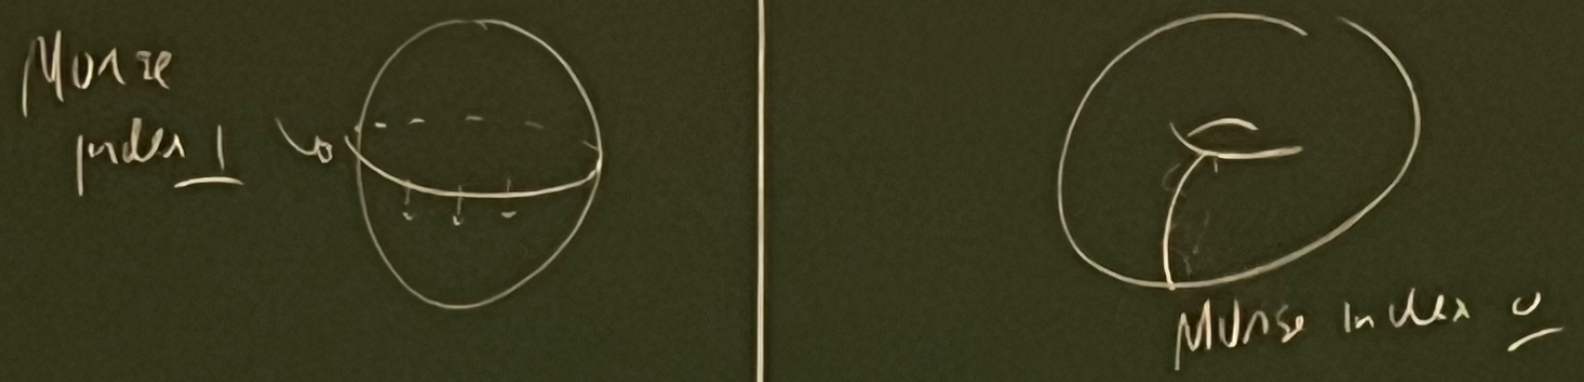
\includegraphics[width=0.7\textwidth]{systolic2}
\end{figure}
\end{remark}

How to find \(\Sigma_k\)? You make an \textit{educated guess} of what \(\operatorname{area}_g\Sigma_k\) should be.

Almgren in the 60's showed that the space of all trivial closed hypersurfaces,
\(\mathcal{Z}_n(M)\) is weakly homotopic to \(\mathbb{R}P^{\infty}\). So a lot of cohomology.

For a fixed metric \(g\), minimal hypersurfaces are critical points of
\[\operatorname{area}_g: \mathcal{Z}_n(M) \to [0,+\infty)\]

The educated guess is that the area corresponds to
smallest \(L\) so that \(\lambda^k \neq 0 \) on \(\{ \Sigma\in \mathcal{Z}:\operatorname{area}(\Sigma)\leq L\}\)

\begin{figure}[H]
	\centering
	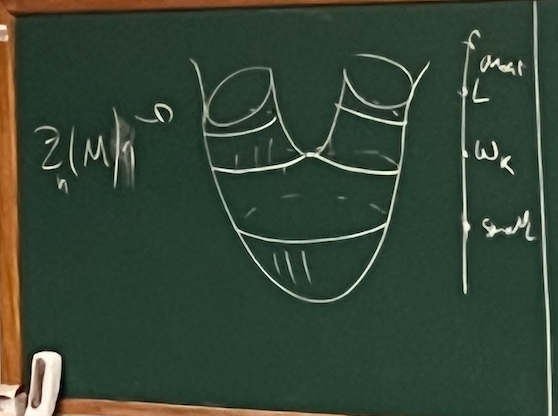
\includegraphics[width=0.4\textwidth]{systolic}
	\caption*{looks like some sort of Morse theory approach}
\end{figure}

\subsection{Zoll metrics}
A classical question in the theory of geodesics is to know to which extent the length of closed geodesics determines the ambient metric. For surfaces the answer depends on the curvature. Negative, flat, yes. Positive, no!

\begin{question}[dani]\leavevmode
What is Zoll metric? What is volume spectrum? (I stopped following at this point.)
\end{question}

\clearpage\phantomsection\stepcounter{section}\addcontentsline{toc}{section}{\thesection\quad Lie Groupoids: Foundations, Advances, and Future Directions}\addtocontents{toc}{\hspace{1em}\textit{Matias del Hoyo, \hspace{.2 em}UFRJ,\hspace{.5em}March 21, 2025, Seminário das Sextas}\par}
{\Huge Lie Groupoids: Foundations, Advances, and Future Directions}

\hfill{\Large Matias del Hoyo}

{\Large \hfill UFRJ}

\hfill{\large March 21, 2025

\hfill \textit{Seminário das Sextas}}
\vspace{2em}

\begin{thing6}{Abstract}
Lie groupoids are central to modern geometry and mathematical physics, connecting differential geometry, topology, and dynamical systems. Based on a recent chapter co-authored with H. Bursztyn for the \href{https://www.sciencedirect.com/science/article/abs/pii/B9780323957038000240}{Encyclopedia of Mathematical Physics} this talk will explore the foundations of Lie groupoids, their interactions with related structures like Lie algebroids and Poisson manifolds, and highlight recent advances and emerging research directions in the field.
\end{thing6}
\vspace{2em}

\vspace{2em}
\subsection{Lie groupoids}

\begin{defn}\leavevmode
A \textit{\textbf{Lie groupoid}} \(G \substack{\to\\\to} M\) consists of manifolds \(G\), \(M\), submersions \(s,t:G \to M\) and a multiplication \(m\) with unit \(u\) and inverse \(i\) 
\begin{align*}
m: G \times_M G&\to G\qquad (z \overset{g}{\leftarrow }y, y\overset{g}{\leftarrow } x )\mapsto  (z\overset{hg}{\leftarrow }x)\\
u:M & \to G\qquad \qquad x \mapsto (x \overset{1_x}{\leftarrow }x)\\
i:G&\to G\qquad \qquad (y \overset{g}{\leftarrow }x)\mapsto (x\overset{g^{-1}}{\leftarrow }y)
\end{align*}
A \textit{\textbf{morphism}} \(\phi:(\tilde{G}\substack{\to\\\to}M) \to (G \substack{\to\\\to}M)\) consists of maps \(\phi_1:\tilde{G} \to G\), \(\phi_2:\tilde{M} \to M\) preserving source, target, multiplication and units.
\end{defn}

\subsection{Examples}

\begin{example}\leavevmode
\begin{itemize}
\item For \(M\) manifold:
\begin{itemize}
\item \(M\substack{\to\\\to}M\) unit groupoid.
\item \(M \times M \substack{\to\\\to} M\) pair groupoid.
\item \(\pi_{1}(M)\substack{\to\\\to}M\) fundamental groupoid.
\end{itemize}
\item \(G\) Lie group: \(G \substack{\to\\\to} *\) Lie group

\item \(q:M \to N\) submersion: \(M \times_M \substack{\to\\\to}M\) submersion groupoid. Ex: \(\mathcal{U}=\{U_i\}\) open cover \(\rightsquigarrow \) \(\coprod U_{ji}\substack{\to\\\to}\coprod U_i\) \v Chech groupoid.
\item \(G \mathbb{y} M\) action:  \(G \times M \substack{\to\\\to}M\) action groupoid.
\item \(X \in \Gamma(TM)\): \(U_X \subset \mathbb{R}\times M \substack{\to\\\to}M\) flow gruopoid.
\item \(P \to M\) principal bundle: \((P\times P)/G \substack{\to\\\to}M\) gauge groupoid.
\item  \(F \subset M\) foliation:
	\begin{itemize}
	\item \(\operatorname{Mon}F \substack{\to\\\to} M\) monodromy groupoid
	\item \(\operatorname{Hol}M \substack{\to\\\to} M\) holonomy groupoid.
\item \(V \to M\) vector bundle: \(\mathsf{GL}(V)\substack{\to\\\to}M\) bigeneral linear groupoid.
	\end{itemize}
\end{itemize}
\end{example}

\subsection{Actions and representations}

Here's one of the key ideas: relation between group and groupoid. Groups in geometry serve to model symmetries of a space:
\[\text{group } G \substack{\to\\\to} * \leftrightsquigarrow \text{symmetries of a space }E \to * \]
And groupoids model symmetries of a \textit{family} parametrized by \(M\):
\[\text{groupoid }G \substack{\to\\\to}M \leftrightsquigarrow \text{symmetries of a family }E \to M\]
\begin{defn}\leavevmode
Given \(G\substack{\to\\\to}M\) a Lie grouoid and \(E \to M\) a surjective submersion, a \textit{\textbf{groupoid action}} \(\rho:G \mathbb{y} E\) is a map such that \(\rho_{1_x}=\operatorname{id}_{E_x}\) and \(\rho_h\rho_g=\rho_{gh}\):
\[\rho:G \times_M E \to E\qquad (y\leftarrow x,e/x)\mapsto \rho_g(e)/y\]
It is a \textit{\textbf{representation}} if \(E \to M\) vector bundle and \(\rho_g E_x \to E_y\) linear.
\end{defn}

\begin{example}\leavevmode
\begin{itemize}
\item The \textit{\textbf{parallel action}}. Take a vector bundle with a flat connection. Then the fundamental groupoid \textit{acts by parallel transport}, i.e. \((E \to M, \nabla)\) is a groupoid action \((\pi_{1}(M)\substack{\to\\\to}M \mathbb{y} (E \to M)\). Notice this is \textit{not} a group action, it's naturally a groupoid action.
\item A \textit{\textbf{Hamiltonian action}} \(G \mathbb{y}(M,\omega)\) on a symplectic manifold is an action of the action groupoid \((G \times \mathfrak{g}^*\substack{\to\\\to}\mathfrak{g}^*\mathbb{y}(M\to \mathfrak{g}^*)\).
\item The \textit{\textbf{(linear) holonomy}} of a foliation \(F \subset TM\) is a representation of the monodromy groupoid \((\operatorname{Mon}(F) \substack{\to\\\to}M \mathbb{y}(TM/F \to M)\).
\end{itemize}\end{example}

\subsection{Groupoid fibrations}
A representation \((G\substack{\to\\\to}M)\mathbb{y}(E \to M)\) gives rise to a groupoid morphism with a (unique) lift of arrows:
\[\begin{tikzcd}
	G \times_M E \substack{\to\\\to}E\arrow[d]&\leavevmode& e\arrow[l,"\rho(g\text{,} e)",red,swap]\\
	G\substack{\to\\\to}M& y& x\arrow[l,"g",swap]
\end{tikzcd}\]
A \textit{\textbf{fibration}} \(\Gamma \substack{\to\\\to}E) \to (G \substack{\to\\\to}M)\) is a morphism with (non-necessarily unique) lift of arrows. A \textit{\textbf{VB-groupoid}} is a linear fibration (called like this for historical reasons).

\begin{example}\leavevmode
\begin{itemize}
\item A usual representation \((G \ltimes_E \substack{\to\\\to}E) \to (G \substack{\to\\\to} M)\)
\item The tangent and the cotangent groupoid \((TG \substack{\to\\\to} TM) \to (G \substack{\to\\\to}M)\) and \((T^*G \substack{\to\\\to}A^*) \to (G\substack{\to\\\to}M)\)
\end{itemize}
\end{example}
\begin{thm}[Grothendieck;Gacria-Saz,Mehta;dH,Ortiz]\leavevmode
There is a 1-1 correspondence between VB-groupoids \(\Gamma\to E\) over \(G \substack{\to\\\to}M\) and {\color{2}representations up to homotopy} \(G\mathbb{y}(C \oplus  E \to M)\).
\end{thm}

\subsection{Nerve and cohomology}

Given \(G \substack{\to\\\to} M\) Lie groupoid, its \textit{\textbf{nerve}} \((NG_n,d_i,s_j)\) is the simplicial manifold
\begin{itemize}
\item \(n\)-simplices: \(NG_n=\{x_n \overset{g_n}{\leftarrow}x_{n-1}\overset{g_{n-1}}{\leftarrow}\cdots \overset{g_2}{\leftarrow}x_1\overset{g_1}{\leftarrow}x_0\}\) 
\item Faces \(d_i:NG_n \to NG_{n-1}\) compose two arrows (or forget one)
\item Degeneracies \(s_j:NG_n \to NG_{n+1}\) insert and identity.
\end{itemize}
The \textit{\textbf{groupoid DGA}} is \(C(G)=(sin(NG_\bullet),\cup ,\partial=\sum_{i}(-1)^i d_i^*)\). The \textit{\textbf{groupoid cohomology}} is \(H^{n}(G)=H^{n}(C(G))\).


\subsection{Linearization problem}
\begin{remark}\leavevmode
Here was discussed a notion of \textit{proper groupoid}, which have analogous properties of proper Lie groups: quotient is Hausdorff and admits a Haar measure.
\end{remark}
\subsection{Metric on a Lie groupoid}

\begin{defn}\leavevmode
A \textit{\textbf{metric}} on \(G \substack{\to\\\to}M\) is a metric \(\eta^{(2)}\) on \(NG_2=G \times_M G\) such that the face maps are Riemannian submersions…
\end{defn}
It's actually a \textit{system of metric}, making source, target, multiplication Riemannian submersions.

\begin{thm}[dH-Fernandes, 2018]\leavevmode
Every proper Lie groupoid admits a metric, and a metric yields linearizations through the exponential maps.
\end{thm}

\begin{remark}\leavevmode
How to construct a invariant metric from any metric.
\end{remark}

\begin{remark}[About the future]\leavevmode
It's not yet clear how to define a proper higher Lie groupoid. Speaker is trying to develop geometry for higher Lie groupoids.
\end{remark}

\subsection{Part 2}

\subsection{Abstract Lie algebroids}

\begin{defn}\leavevmode
	A \textit{\textbf{Lie algebroid}} \(A \implies  M\) is a vector bundle \(A \to M\) with a Lie bracket \([\cdot,\cdot]\) on \(\Gamma(A)\) and a linear map \(\rho:A \to TM\) satisfying Leibniz rule
	\[[\alpha,f \beta]=f[\alpha,\beta]+\rho(\alpha)(f)\beta\qquad \qquad \alpha, \beta \in \Gamma(A),f \in C^\infty(M)\]
If 	
\end{defn}

\begin{remark}\leavevmode
Also \textit{\textbf{higher Lie algebras}} have been defined.
\end{remark}

\section{Last slide}
There were several slides in between…

\begin{thm}[Crainic-Fernandes]\leavevmode
There is a 1-1 correspodnence between (\(s\)-simply connected) symplectic Lie groupoids and (integrable) Poisson manifolds.
\end{thm}

Why symplectic groupoid and Poisson manifolds? They seem to be different objects. Theese (which?) induce Lie algebra. Because cotangent structure 

\begin{quotation}
``Poisson manifold induce a symplectic lie algebra." ``Integration of symplectic algebra is symplectic group"
\end{quotation}


\end{document}
